%!TEX root = ./main.tex



\begin{definition}
    Un poliedro es una 3-bola cerrada, tal que en su frontera se encuentre marcada con un grafo finito, tal que la regiones complementarias llamadas caras son simplemente conexas.
\end{definition}
Prácticamente cualquier dibujo clásico que se puede hacer (de manera natural sin estar buscando no ejemplos) resulta ser un ejemplo de poliedro
\begin{figure}[H]
    \centering
    
%!TEX root = ./main.tex





\tikzset{every picture/.style={line width=0.75pt}} %set default line width to 0.75pt        

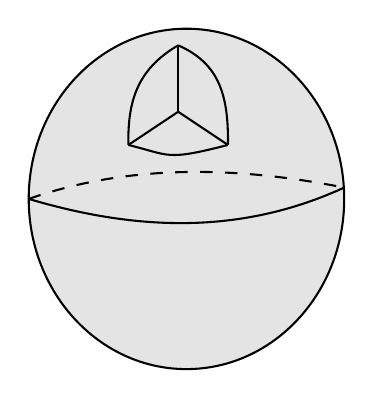
\begin{tikzpicture}[x=0.75pt,y=0.75pt,yscale=-0.8,xscale=0.8]
%uncomment if require: \path (0,877); %set diagram left start at 0, and has height of 877

%Shape: Ellipse [id:dp0928071191771559] 
\draw  [fill={rgb, 255:red, 155; green, 155; blue, 155 }  ,fill opacity=0.27 ] (220,122.5) .. controls (220,65.89) and (262.53,20) .. (315,20) .. controls (367.47,20) and (410,65.89) .. (410,122.5) .. controls (410,179.11) and (367.47,225) .. (315,225) .. controls (262.53,225) and (220,179.11) .. (220,122.5) -- cycle ;
%Curve Lines [id:da13418485162745786] 
\draw    (220,122.5) .. controls (285.87,142.09) and (348.36,143.91) .. (410,115.67) ;
%Curve Lines [id:da5341258541218854] 
\draw  [dash pattern={on 4.5pt off 4.5pt}]  (220,122.5) .. controls (284.18,100.18) and (350.04,103.82) .. (410,115.67) ;
%Straight Lines [id:da3427735018941048] 
\draw    (280,90) -- (310,70) ;
%Straight Lines [id:da6109826278772268] 
\draw    (310,70) -- (340,90) ;
%Straight Lines [id:da31209815320417755] 
\draw    (310,30) -- (310,70) ;
%Curve Lines [id:da4696149880079775] 
\draw    (280,90) .. controls (279.67,65) and (284.33,45) .. (310,30) ;
%Curve Lines [id:da0013412730978942244] 
\draw    (310,30) .. controls (335,41) and (340.33,60.33) .. (340,90) ;
%Curve Lines [id:da5680668023106804] 
\draw    (280,90) .. controls (305.67,96.33) and (302.33,99.67) .. (340,90) ;




\end{tikzpicture}
    \caption{Ejemplo de poliedro}
\end{figure}
La condición final esta puesta para asegurar que las caras si se comporten como discos poligonales para tener un análogo de la imagen usual que uno suele tener de poliedro, mas si no la tuviéramos podemos hacer uno de esos dibujos que mencionábamos antes.
\begin{figure}[H]
    \centering
    
%!TEX root = ./main.tex



\tikzset{every picture/.style={line width=0.75pt}} %set default line width to 0.75pt        

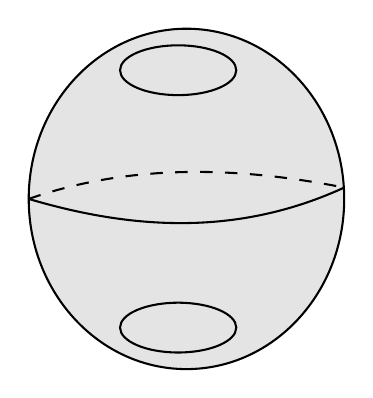
\begin{tikzpicture}[x=0.75pt,y=0.75pt,yscale=-0.8,xscale=0.8]
%uncomment if require: \path (0,877); %set diagram left start at 0, and has height of 877

%Shape: Ellipse [id:dp0928071191771559] 
\draw  [fill={rgb, 255:red, 155; green, 155; blue, 155 }  ,fill opacity=0.27 ] (230,122.5) .. controls (230,65.89) and (272.53,20) .. (325,20) .. controls (377.47,20) and (420,65.89) .. (420,122.5) .. controls (420,179.11) and (377.47,225) .. (325,225) .. controls (272.53,225) and (230,179.11) .. (230,122.5) -- cycle ;
%Curve Lines [id:da13418485162745786] 
\draw    (230,122.5) .. controls (295.87,142.09) and (358.36,143.91) .. (420,115.67) ;
%Curve Lines [id:da5341258541218854] 
\draw  [dash pattern={on 4.5pt off 4.5pt}]  (230,122.5) .. controls (294.18,100.18) and (360.04,103.82) .. (420,115.67) ;
%Shape: Ellipse [id:dp9147901422013078] 
\draw   (285,45) .. controls (285,36.72) and (300.67,30) .. (320,30) .. controls (339.33,30) and (355,36.72) .. (355,45) .. controls (355,53.28) and (339.33,60) .. (320,60) .. controls (300.67,60) and (285,53.28) .. (285,45) -- cycle ;
%Shape: Ellipse [id:dp5524598870994889] 
\draw   (285,200) .. controls (285,191.72) and (300.67,185) .. (320,185) .. controls (339.33,185) and (355,191.72) .. (355,200) .. controls (355,208.28) and (339.33,215) .. (320,215) .. controls (300.67,215) and (285,208.28) .. (285,200) -- cycle ;




\end{tikzpicture}
    \caption{Grafo que genera una región que no es simplemente conexa}
\end{figure}
Como nuestro propósito es estudiar los complementos de los nudos en $S^3$ si lo pensamos bien la información que nos da el nudo es aquello que falta, es decir son huecos en la descomposición, esto motiva la siguiente definición. 
\begin{definition}
    Un poliedro ideal es un poliedro en el cual removemos todos los puntos que antes habíamos marcado como vértices.
\end{definition}

Nuestra idea sera cortar $S^3\setminus K$ en dos poliedros ideales, así tendríamos  una descripción del complemento como el pegado de dos estructuras mucho mas sencillas de comprender (en particular de visualizar).\\

Una primera intuición geométrica que nos da la construcción es la siguiente, Consideremos el siguiente diagrama del nudo de 8
\begin{figure}[H]
    \centering
    
%!TEX root = ./main.tex



\tikzset{every picture/.style={line width=0.75pt}} %set default line width to 0.75pt        

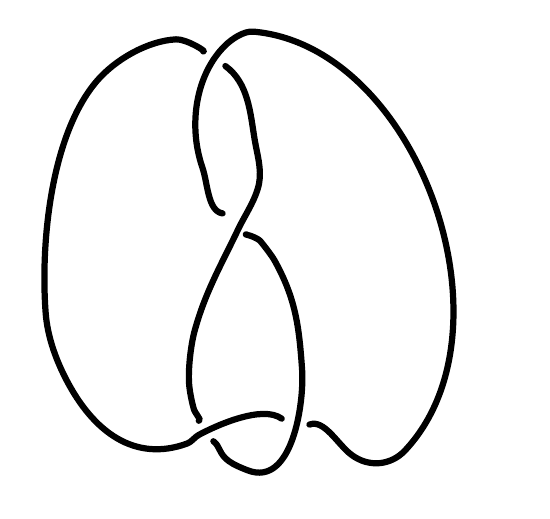
\begin{tikzpicture}[x=0.75pt,y=0.75pt,yscale=-0.85,xscale=0.85]
%uncomment if require: \path (0,877); %set diagram left start at 0, and has height of 877

%Shape: Free Drawing [id:dp0005319926756554016] 
\draw  [line width=2.25] [line join = round][line cap = round] (298.71,113.07) .. controls (290.26,111.76) and (290.37,96.06) .. (287.28,87.1) .. controls (278.97,62.96) and (283.59,34.1) .. (300.2,17.86) .. controls (303.92,14.22) and (310.73,9.55) .. (316.2,10.03) .. controls (409.49,18.29) and (466.49,178.81) .. (402.12,247.44) .. controls (394.25,255.83) and (381.75,257.34) .. (371.76,249.89) .. controls (363.9,244.03) and (356.41,229.52) .. (347.94,232.75) ;
%Shape: Free Drawing [id:dp4987515250733162] 
\draw  [line width=2.25] [line join = round][line cap = round] (332.24,229.4) .. controls (321.28,221.4) and (294.93,233.34) .. (285.13,238.66) .. controls (282.8,239.92) and (281.19,242.57) .. (278.71,243.48) .. controls (249.19,254.28) and (225.41,237.38) .. (209.61,206.31) .. controls (203.85,194.99) and (199.42,182.36) .. (198.44,169.63) .. controls (195.36,129.43) and (201.51,68.2) .. (227.52,37.92) .. controls (237.95,25.79) and (256.3,15.25) .. (272.26,14.4) .. controls (278.18,14.08) and (290.4,21.7) .. (287.75,21.28) ;
%Shape: Free Drawing [id:dp6231462806336996] 
\draw  [line width=2.25] [line join = round][line cap = round] (300.29,29.52) .. controls (313.33,39.03) and (314.36,55.83) .. (316.87,71.08) .. controls (318.17,78.94) and (320.99,87.94) .. (319.38,96.11) .. controls (317.59,105.21) and (311.25,114.25) .. (307.55,122.05) .. controls (298.18,141.77) and (288.6,158.03) .. (282.65,180.47) .. controls (280.81,187.4) and (278.84,202.37) .. (279.89,211.4) .. controls (280.38,215.6) and (281.27,219.79) .. (282.38,223.89) .. controls (283.01,226.24) and (287.39,230.94) .. (285.22,230.6) ;
%Shape: Free Drawing [id:dp34435703317452426] 
\draw  [line width=2.25] [line join = round][line cap = round] (293.48,242.2) .. controls (297.43,245.08) and (296.48,249.26) .. (302.16,253.4) .. controls (305.44,255.79) and (309.19,257.21) .. (312.85,258.65) .. controls (338.56,268.73) and (345.04,219.7) .. (343.78,201.62) .. controls (342.05,176.65) and (340.06,161.14) .. (328.08,139.58) .. controls (326.46,136.67) and (320.37,128.91) .. (319.8,128.44) .. controls (316.42,125.63) and (309.39,124.58) .. (312.66,125.09) ;
%Shape: Free Drawing [id:dp9595901252421886] 
\draw  [color={rgb, 255:red, 255; green, 255; blue, 255 }  ,draw opacity=1 ][line width=2.25] [line join = round][line cap = round] (295.15,117.89) .. controls (294.9,117.98) and (294.33,118.06) .. (294.34,117.76) ;
%Shape: Free Drawing [id:dp1969537050250879] 
\draw  [draw opacity=0][line width=2.25] [line join = round][line cap = round] (426.53,66.18) .. controls (426.65,66.26) and (427.07,66.26) .. (426.94,66.24) ;
%Shape: Free Drawing [id:dp026195381751755398] 
\draw  [draw opacity=0][line width=2.25] [line join = round][line cap = round] (300.82,112.05) .. controls (298.16,113.06) and (297.03,115.75) .. (296.34,118.52) ;
%Shape: Free Drawing [id:dp45027773036340213] 
\draw  [draw opacity=0][line width=2.25] [line join = round][line cap = round] (299.5,113.63) .. controls (292.93,121.91) and (291.72,122.28) .. (294.04,122.64) ;
%Shape: Free Drawing [id:dp42616248151326175] 
\draw  [draw opacity=0][line width=2.25] [line join = round][line cap = round] (299.96,112.81) .. controls (297.93,115.24) and (295.36,117.35) .. (294.18,120.42) ;
%Shape: Free Drawing [id:dp4649779193663184] 
\draw  [draw opacity=0][line width=2.25] [line join = round][line cap = round] (288.84,231.61) .. controls (287.29,232.56) and (285.87,233.82) .. (284.18,234.47) .. controls (283.73,234.64) and (284.58,233.19) .. (285.07,233.26) ;
%Shape: Free Drawing [id:dp48154694518391594] 
\draw  [draw opacity=0][line width=2.25] [line join = round][line cap = round] (281.37,233.59) .. controls (284.36,231.84) and (286.8,227.71) .. (290.28,228.25) ;
%Shape: Free Drawing [id:dp8989735988593472] 
\draw  [draw opacity=0][line width=2.25] [line join = round][line cap = round] (285.58,231.55) .. controls (287.76,231.89) and (289.57,229.92) .. (291.46,228.88) ;
%Shape: Free Drawing [id:dp8922120977301046] 
\draw  [draw opacity=0][line width=2.25] [line join = round][line cap = round] (284.02,230.41) .. controls (285.23,230.16) and (290.6,229.69) .. (290.74,227.42) ;
%Shape: Free Drawing [id:dp5528703258533438] 
\draw  [draw opacity=0][line width=2.25] [line join = round][line cap = round] (284.37,231.36) .. controls (286.58,230.33) and (292.29,228.72) .. (292.52,225.01) ;
%Shape: Free Drawing [id:dp9013988558965794] 
\draw  [draw opacity=0][line width=2.25] [line join = round][line cap = round] (284.31,232.25) .. controls (287.24,229.93) and (290.03,227.39) .. (292.55,224.57) ;
%Shape: Free Drawing [id:dp8372444458576085] 
\draw  [draw opacity=0][line width=2.25] [line join = round][line cap = round] (283.51,232.13) .. controls (288.08,228.65) and (290.79,224.57) .. (293.69,219.37) ;
%Shape: Free Drawing [id:dp8237859994697239] 
\draw  [draw opacity=0][line width=2.25] [line join = round][line cap = round] (191.28,50.96) .. controls (190.75,50.66) and (190.28,50.16) .. (190,49.59) ;




\end{tikzpicture}
    \caption{Proyección del nudo de 8}
\end{figure}
La idea subyacente sera considerar el diagrama en un plano proyección con cierto volumen, para que de esta forma si bien sea prácticamente una proyección en términos de visualización en realidad sea el mismo nudo original embebido en $S^2\times[-\varepsilon,\varepsilon]$, para $\varepsilon>0$, tal que todo eso este contenido en $S^3$, una ilustración que describe eso es la siguiente
\begin{figure}[H]
    \centering
    
%!TEX root = ./main.tex



\tikzset{every picture/.style={line width=0.75pt}} %set default line width to 0.75pt        

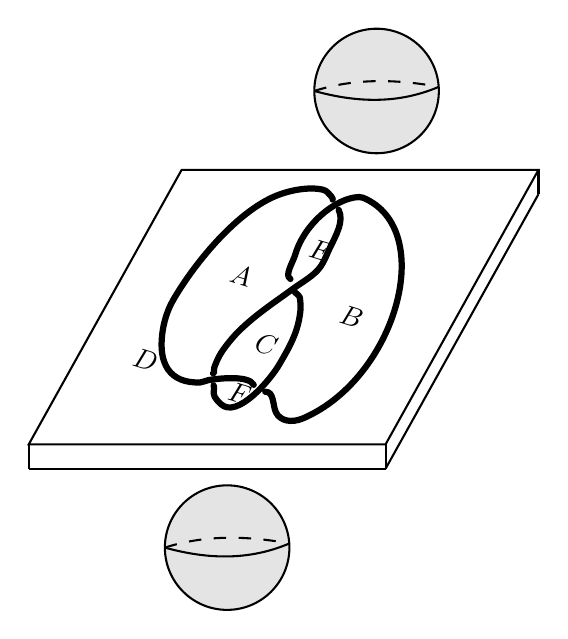
\begin{tikzpicture}[x=0.75pt,y=0.75pt,yscale=-0.8,xscale=0.8]
%uncomment if require: \path (0,877); %set diagram left start at 0, and has height of 877

%Shape: Free Drawing [id:dp7347232652227033] 
\draw  [line width=2.25] [line join = round][line cap = round] (340.64,155.74) .. controls (336.75,153.74) and (342.11,145.88) .. (343.56,140.89) .. controls (347.45,127.45) and (359.56,113.7) .. (373.56,108.19) .. controls (376.69,106.96) and (381.76,105.7) .. (384.4,106.81) .. controls (429.43,125.8) and (404.44,215.43) .. (348.27,239.63) .. controls (341.4,242.59) and (334.48,241.36) .. (331.88,236.03) .. controls (329.83,231.84) and (330.89,223.37) .. (325.46,223.64) ;
%Shape: Free Drawing [id:dp9263733489395964] 
\draw  [line width=2.25] [line join = round][line cap = round] (318.53,219.46) .. controls (315.61,213.7) and (298.07,215.5) .. (291.25,216.61) .. controls (289.63,216.88) and (287.91,217.95) .. (286.33,218.01) .. controls (267.56,218.73) and (261.07,206.47) .. (263.47,188.36) .. controls (264.34,181.76) and (266.33,174.72) .. (270.13,168.17) .. controls (282.13,147.51) and (305.96,117.75) .. (329.52,106.7) .. controls (338.96,102.27) and (351.92,99.9) .. (360.39,102.01) .. controls (363.53,102.79) and (367.22,108.56) .. (366,107.93) ;
%Shape: Free Drawing [id:dp06457306751650549] 
\draw  [line width=2.25] [line join = round][line cap = round] (369.66,114.06) .. controls (373.13,120.9) and (367.98,129.5) .. (364.12,137.55) .. controls (362.13,141.7) and (360.53,146.67) .. (356.95,150.51) .. controls (352.96,154.8) and (346.66,158.33) .. (342.12,161.65) .. controls (330.67,170.06) and (320.27,176.7) .. (309.64,187.02) .. controls (306.36,190.2) and (300.29,197.41) .. (297.78,202.11) .. controls (296.61,204.29) and (295.66,206.53) .. (294.84,208.77) .. controls (294.37,210.05) and (295.02,213.1) .. (294.03,212.59) ;
%Shape: Free Drawing [id:dp21552600534807442] 
\draw  [line width=2.25] [line join = round][line cap = round] (294.34,219.72) .. controls (295.39,221.79) and (293.49,223.74) .. (295.01,226.72) .. controls (295.88,228.44) and (297.32,229.75) .. (298.71,231.06) .. controls (308.48,240.2) and (328.36,216.63) .. (333.82,207.35) .. controls (341.37,194.54) and (345.59,186.45) .. (346.73,173.72) .. controls (346.88,172) and (346.38,167.14) .. (346.25,166.81) .. controls (345.46,164.86) and (342.22,163.22) .. (343.72,163.99) ;
%Shape: Free Drawing [id:dp7149381563661258] 
\draw  [color={rgb, 255:red, 255; green, 255; blue, 255 }  ,draw opacity=1 ][line width=2.25] [line join = round][line cap = round] (337.18,157.59) .. controls (337.02,157.6) and (336.7,157.55) .. (336.81,157.4) ;
%Shape: Free Drawing [id:dp22964569689630154] 
\draw  [draw opacity=0][line width=2.25] [line join = round][line cap = round] (422.02,152.55) .. controls (422.05,152.61) and (422.27,152.68) .. (422.2,152.64) ;
%Shape: Free Drawing [id:dp10065941420052993] 
\draw  [draw opacity=0][line width=2.25] [line join = round][line cap = round] (342.06,155.56) .. controls (340.35,155.65) and (338.87,156.82) .. (337.58,158.1) ;
%Shape: Free Drawing [id:dp3497860993106495] 
\draw  [draw opacity=0][line width=2.25] [line join = round][line cap = round] (340.85,156.15) .. controls (334.68,159.26) and (333.94,159.25) .. (335,159.8) ;
%Shape: Free Drawing [id:dp579495330613402] 
\draw  [draw opacity=0][line width=2.25] [line join = round][line cap = round] (341.36,155.81) .. controls (339.5,156.71) and (337.47,157.35) .. (335.82,158.71) ;
%Shape: Free Drawing [id:dp7142046075462641] 
\draw  [draw opacity=0][line width=2.25] [line join = round][line cap = round] (295.53,213.66) .. controls (294.41,213.89) and (293.26,214.3) .. (292.17,214.36) .. controls (291.88,214.37) and (292.81,213.78) .. (293.03,213.89) ;
%Shape: Free Drawing [id:dp36059894867560727] 
\draw  [draw opacity=0][line width=2.25] [line join = round][line cap = round] (291.03,213.47) .. controls (293.15,213.07) and (295.8,211.38) .. (297.4,212.2) ;
%Shape: Free Drawing [id:dp6910674550747714] 
\draw  [draw opacity=0][line width=2.25] [line join = round][line cap = round] (293.88,213.12) .. controls (294.87,213.63) and (296.47,212.93) .. (297.79,212.71) ;
%Shape: Free Drawing [id:dp5927274501309536] 
\draw  [draw opacity=0][line width=2.25] [line join = round][line cap = round] (293.46,212.3) .. controls (294.16,212.36) and (297.07,212.98) .. (297.91,211.86) ;
%Shape: Free Drawing [id:dp5667950092933809] 
\draw  [draw opacity=0][line width=2.25] [line join = round][line cap = round] (293.32,212.83) .. controls (294.8,212.66) and (298.27,212.76) .. (299.64,210.94) ;
%Shape: Free Drawing [id:dp23387142797305527] 
\draw  [draw opacity=0][line width=2.25] [line join = round][line cap = round] (292.99,213.26) .. controls (295.27,212.57) and (297.56,211.74) .. (299.81,210.72) ;
%Shape: Free Drawing [id:dp009814050173147182] 
\draw  [draw opacity=0][line width=2.25] [line join = round][line cap = round] (292.62,213.07) .. controls (296.13,212.06) and (298.9,210.44) .. (302.15,208.29) ;
%Shape: Free Drawing [id:dp1531990322186717] 
\draw  [draw opacity=0][line width=2.25] [line join = round][line cap = round] (306.53,107.47) .. controls (306.36,107.24) and (306.29,106.91) .. (306.34,106.58) ;

%Shape: Parallelogram [id:dp602722874823763] 
\draw   (275.1,90) -- (490,90) -- (397.9,255.35) -- (183,255.35) -- cycle ;
%Straight Lines [id:da33965271518677576] 
\draw    (183,255.35) -- (183,270) ;
%Straight Lines [id:da5238934226743897] 
\draw    (397.9,255.35) -- (397.9,270) ;
%Straight Lines [id:da46592613323086984] 
\draw    (490,90) -- (490,104.65) ;
%Straight Lines [id:da03324567448990312] 
\draw    (183,270) -- (397.97,270) ;
%Straight Lines [id:da05494519914066254] 
\draw    (397.9,270) -- (490,104.65) ;
%Shape: Circle [id:dp6719648380552748] 
\draw  [fill={rgb, 255:red, 155; green, 155; blue, 155 }  ,fill opacity=0.27 ] (355,42.5) .. controls (355,21.79) and (371.79,5) .. (392.5,5) .. controls (413.21,5) and (430,21.79) .. (430,42.5) .. controls (430,63.21) and (413.21,80) .. (392.5,80) .. controls (371.79,80) and (355,63.21) .. (355,42.5) -- cycle ;
%Curve Lines [id:da7420886829816177] 
\draw    (355,42.5) .. controls (381,49.67) and (405.67,50.33) .. (430,40) ;
%Curve Lines [id:da9534326817781857] 
\draw  [dash pattern={on 4.5pt off 4.5pt}]  (355,42.5) .. controls (380.33,34.33) and (406.33,35.67) .. (430,40) ;
%Shape: Circle [id:dp6798222831973407] 
\draw  [fill={rgb, 255:red, 155; green, 155; blue, 155 }  ,fill opacity=0.27 ] (265,317.5) .. controls (265,296.79) and (281.79,280) .. (302.5,280) .. controls (323.21,280) and (340,296.79) .. (340,317.5) .. controls (340,338.21) and (323.21,355) .. (302.5,355) .. controls (281.79,355) and (265,338.21) .. (265,317.5) -- cycle ;
%Curve Lines [id:da8454704520111102] 
\draw    (265,317.5) .. controls (291,324.67) and (315.67,325.33) .. (340,315) ;
%Curve Lines [id:da3154394219916593] 
\draw  [dash pattern={on 4.5pt off 4.5pt}]  (265,317.5) .. controls (290.33,309.33) and (316.33,310.67) .. (340,315) ;

% Text Node
\draw (305.43,143.97) node [anchor=north west][inner sep=0.75pt]  [rotate=-17.24]  {$A$};
% Text Node
\draw (371.51,168.5) node [anchor=north west][inner sep=0.75pt]  [rotate=-17.24]  {$B$};
% Text Node
\draw (320.48,185.73) node [anchor=north west][inner sep=0.75pt]  [rotate=-17.24]  {$C$};
% Text Node
\draw (246.92,194.77) node [anchor=north west][inner sep=0.75pt]  [rotate=-17.24]  {$D$};
% Text Node
\draw (353.07,129.16) node [anchor=north west][inner sep=0.75pt]  [rotate=-17.24]  {$E$};
% Text Node
\draw (304.31,214.98) node [anchor=north west][inner sep=0.75pt]  [rotate=-17.24]  {$F$};


\end{tikzpicture}
    \caption{Dos 3 bolas inflándose hasta chocar con el nudo}
\end{figure}
Los globos que se encuentran sobre y debajo del plano representaran las 3-bolas que identificaremos para que por medio de la función de pegado codifiquen $S^3\setminus K$. La idea sera inflar estas hasta que se encuentren las fronteras de ambas, la pregunta que surge es estas donde se encontraran y de que manera se producirá la identificación. Observemos que en una región local del diagrama donde no halla un cruce al expandirse los globos estos se verán de la siguiente manera
\begin{figure}[H]
    \centering
    
%!TEX root = ./main.tex



\tikzset{every picture/.style={line width=0.75pt}} %set default line width to 0.75pt        

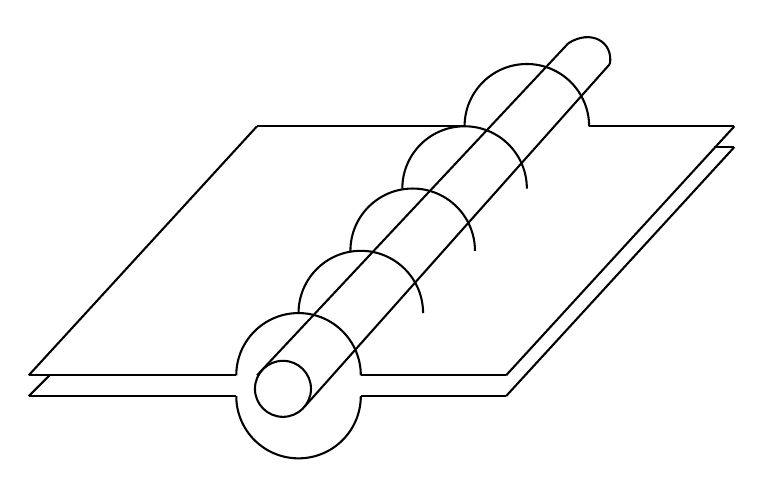
\begin{tikzpicture}[x=0.75pt,y=0.75pt,yscale=-1,xscale=1]
%uncomment if require: \path (0,877); %set diagram left start at 0, and has height of 877

%Straight Lines [id:da9114133242483868] 
\draw    (130,190) -- (230,190) ;
%Shape: Arc [id:dp76715373468173] 
\draw  [draw opacity=0] (230,190) .. controls (230,173.43) and (243.43,160) .. (260,160) .. controls (276.57,160) and (290,173.43) .. (290,190) -- (260,190) -- cycle ; \draw   (230,190) .. controls (230,173.43) and (243.43,160) .. (260,160) .. controls (276.57,160) and (290,173.43) .. (290,190) ;  
%Straight Lines [id:da5480526040795924] 
\draw    (290,190) -- (360,190) ;
%Straight Lines [id:da8548422928953872] 
\draw    (240,70) -- (130,190) ;
%Straight Lines [id:da9009737644518513] 
\draw    (470,70) -- (360,190) ;
%Shape: Arc [id:dp7906930930707468] 
\draw  [draw opacity=0] (340,70) .. controls (340,53.43) and (353.43,40) .. (370,40) .. controls (386.57,40) and (400,53.43) .. (400,70) -- (370,70) -- cycle ; \draw   (340,70) .. controls (340,53.43) and (353.43,40) .. (370,40) .. controls (386.57,40) and (400,53.43) .. (400,70) ;  
%Straight Lines [id:da7284237450228865] 
\draw    (240,70) -- (340,70) ;
%Straight Lines [id:da9557077871704964] 
\draw    (400,70) -- (470,70) ;
%Shape: Arc [id:dp1517473778529409] 
\draw  [draw opacity=0] (310,100) .. controls (310,83.43) and (323.43,70) .. (340,70) .. controls (356.57,70) and (370,83.43) .. (370,100) -- (340,100) -- cycle ; \draw   (310,100) .. controls (310,83.43) and (323.43,70) .. (340,70) .. controls (356.57,70) and (370,83.43) .. (370,100) ;  
%Shape: Arc [id:dp9007707592571377] 
\draw  [draw opacity=0] (285,130) .. controls (285,113.43) and (298.43,100) .. (315,100) .. controls (331.57,100) and (345,113.43) .. (345,130) -- (315,130) -- cycle ; \draw   (285,130) .. controls (285,113.43) and (298.43,100) .. (315,100) .. controls (331.57,100) and (345,113.43) .. (345,130) ;  
%Shape: Arc [id:dp2562761265277008] 
\draw  [draw opacity=0] (260,160) .. controls (260,143.43) and (273.43,130) .. (290,130) .. controls (306.57,130) and (320,143.43) .. (320,160) -- (290,160) -- cycle ; \draw   (260,160) .. controls (260,143.43) and (273.43,130) .. (290,130) .. controls (306.57,130) and (320,143.43) .. (320,160) ;  
%Straight Lines [id:da12803577030308289] 
\draw    (390,30) -- (240,190) ;
%Shape: Circle [id:dp9817645653301902] 
\draw   (239,196.5) .. controls (239,189.04) and (245.04,183) .. (252.5,183) .. controls (259.96,183) and (266,189.04) .. (266,196.5) .. controls (266,203.96) and (259.96,210) .. (252.5,210) .. controls (245.04,210) and (239,203.96) .. (239,196.5) -- cycle ;
%Straight Lines [id:da8931818284701049] 
\draw    (410,40) -- (263,205) ;
%Curve Lines [id:da20985507457895636] 
\draw    (390,30) .. controls (401,23) and (411.8,29.4) .. (410,40) ;
%Straight Lines [id:da6630076546842583] 
\draw    (130,200) -- (230,200) ;
%Straight Lines [id:da7747329083523316] 
\draw    (140,190) -- (130,200) ;
%Straight Lines [id:da7546070667858217] 
\draw    (290,200) -- (360,200) ;
%Straight Lines [id:da46420675335921213] 
\draw    (470,80) -- (360,200) ;
%Straight Lines [id:da5784934546012858] 
\draw    (460,80) -- (470,80) ;
%Shape: Arc [id:dp14611856141981894] 
\draw  [draw opacity=0] (290,200) .. controls (290,216.57) and (276.57,230) .. (260,230) .. controls (243.43,230) and (230,216.57) .. (230,200) -- (260,200) -- cycle ; \draw   (290,200) .. controls (290,216.57) and (276.57,230) .. (260,230) .. controls (243.43,230) and (230,216.57) .. (230,200) ;  




\end{tikzpicture}
    \caption{Vista local alrededor de una vecindad tubular}
\end{figure}
Al ver esto nos podemos dar una idea de cuales serán las caras de nuestro poliedro para la identificación, precisamente serán las regiones que delimita el diagrama del nudo, así ya tenemos la primera parte identificada, las caras de nuestro poliedro ideal serán las regiones que delimita del diagrama del nudo.\\

La segunda parte que ya tenemos determinada son los vértices ideales del poliedro ya que como mencionamos antes la única información que no esta en nuestra 3-variedad es el nudo en si, entonces los vértices ideales serán las cuerdas del diagrama, mas cuando entremos en detalle del algoritmo veremos como funciona eso.\\

Lo ultimo que nos falta es determinar cuales serán las aristas que rodearan las caras ya determinadas, esto lo podemos ver con la única parte del diagrama del nudo a la cual no hemos prestado tanta atención, la zona de los cruces, para esto presentamos la siguiente ilustracion para dar una intuición de lo que ocurre en esas regiones al inflar los globos.
\begin{figure}[H]
    \centering
    
%!TEX root = ./main.tex



\tikzset{every picture/.style={line width=0.75pt}} %set default line width to 0.75pt        

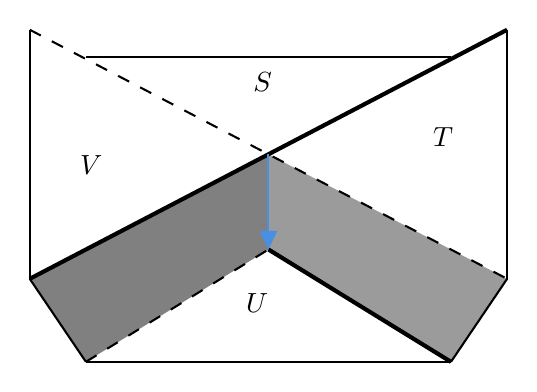
\begin{tikzpicture}[x=0.75pt,y=0.75pt,yscale=-1,xscale=1]
%uncomment if require: \path (0,877); %set diagram left start at 0, and has height of 877

%Straight Lines [id:da6932355685480536] 
\draw [draw opacity=0][fill={rgb, 255:red, 155; green, 155; blue, 155 }  ,fill opacity=1 ]   (412.94,200) -- (440,160) -- (325,100) -- (325,145.87) -- cycle ;
%Straight Lines [id:da1384787451044316] 
\draw [draw opacity=0][fill={rgb, 255:red, 128; green, 128; blue, 128 }  ,fill opacity=1 ]   (210,160) -- (237.06,200) -- (315.46,151.74) -- (325,145.87) -- (325,100) -- cycle ;
%Straight Lines [id:da0741744233702265] 
\draw [line width=1.5]    (210,160) -- (440,40) ;
%Straight Lines [id:da5955578937587962] 
\draw  [dash pattern={on 4.5pt off 4.5pt}]  (210,40) -- (440,160) ;
%Straight Lines [id:da85493541645859] 
\draw    (210,160) -- (237.06,200) ;
%Straight Lines [id:da7842887989072671] 
\draw    (440,160) -- (412.94,200) ;
%Straight Lines [id:da2669884694205853] 
\draw    (210,40) -- (210,160) ;
%Straight Lines [id:da637854901562851] 
\draw    (440,40) -- (440,160) ;
%Straight Lines [id:da7206676036750514] 
\draw [color={rgb, 255:red, 74; green, 144; blue, 226 }  ,draw opacity=1 ]   (325,100) -- (325,142.87) ;
\draw [shift={(325,145.87)}, rotate = 270] [fill={rgb, 255:red, 74; green, 144; blue, 226 }  ,fill opacity=1 ][line width=0.08]  [draw opacity=0] (8.93,-4.29) -- (0,0) -- (8.93,4.29) -- cycle    ;
%Straight Lines [id:da12493325383084064] 
\draw [line width=1.5]    (325,145.87) -- (412.94,200) ;
%Straight Lines [id:da0009226395893477957] 
\draw  [dash pattern={on 4.5pt off 4.5pt}]  (237.06,200) -- (325,145.87) ;
%Straight Lines [id:da06537491608635204] 
\draw    (237.06,200) -- (412.94,200) ;
%Straight Lines [id:da9541213893361323] 
\draw    (237.06,53.33) -- (412.94,53.33) ;

% Text Node
\draw (316.29,59.07) node [anchor=north west][inner sep=0.75pt]    {$S$};
% Text Node
\draw (232.76,99.07) node [anchor=north west][inner sep=0.75pt]    {$V$};
% Text Node
\draw (402.88,85.73) node [anchor=north west][inner sep=0.75pt]    {$T$};
% Text Node
\draw (312.76,165.73) node [anchor=north west][inner sep=0.75pt]    {$U$};


\end{tikzpicture}
    \caption{Dibujo local como segmentos}
\end{figure}
Claramente estas intersecciones están des-suavizadas por propósitos prácticos, pero observe como en la región que se genera entre las cuerdas es una región donde se diferencian tanto las caras del globo de arriba como las de abajo por lo que a cada cruce del diagrama se dotara de una arista con una orientación. Con toda esta información ya podemos plantear un paso a paso completamente basado en el diagrama del nudo (combinatorio) para hacer la descomposición posterior en los dos poliedros.

\begin{block}
Dado un diagrama de un nudo $K$. Este divide el plano en múltiples regiones, designe cada una de estas por algún identificador. Posterior a esto en cada cruce que encuentre en el diagrama dibujaremos aristas (segmentos de recta con orientación) como se muestra a continuación
\begin{figure}[H]
    \centering
    
%!TEX root = ./main.tex



\tikzset{every picture/.style={line width=0.75pt}} %set default line width to 0.75pt        

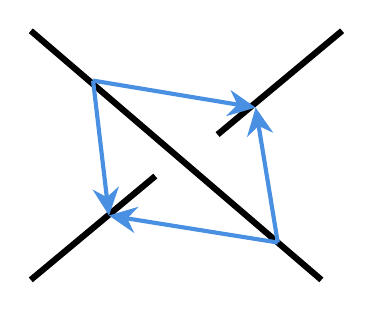
\begin{tikzpicture}[x=0.75pt,y=0.75pt,yscale=-1,xscale=1]
%uncomment if require: \path (0,877); %set diagram left start at 0, and has height of 877

%Straight Lines [id:da46690641073913] 
\draw [line width=2.25]    (210,40) -- (350,160) ;
%Straight Lines [id:da10554492911680236] 
\draw [line width=2.25]    (300,90) -- (360,40) ;
%Straight Lines [id:da8098815627289185] 
\draw [line width=2.25]    (210,160) -- (270,110) ;
%Straight Lines [id:da05962605728576298] 
\draw [color={rgb, 255:red, 74; green, 144; blue, 226 }  ,draw opacity=1 ][line width=1.5]    (329,142) -- (251.62,129.63) ;
\draw [shift={(247.67,129)}, rotate = 9.08] [fill={rgb, 255:red, 74; green, 144; blue, 226 }  ,fill opacity=1 ][line width=0.08]  [draw opacity=0] (13.4,-6.43) -- (0,0) -- (13.4,6.44) -- (8.9,0) -- cycle    ;
%Straight Lines [id:da4600200086141276] 
\draw [color={rgb, 255:red, 74; green, 144; blue, 226 }  ,draw opacity=1 ][line width=1.5]    (240,64) -- (247.2,125.03) ;
\draw [shift={(247.67,129)}, rotate = 263.27] [fill={rgb, 255:red, 74; green, 144; blue, 226 }  ,fill opacity=1 ][line width=0.08]  [draw opacity=0] (13.4,-6.43) -- (0,0) -- (13.4,6.44) -- (8.9,0) -- cycle    ;
%Straight Lines [id:da4794416836174995] 
\draw [color={rgb, 255:red, 74; green, 144; blue, 226 }  ,draw opacity=1 ][line width=1.5]    (240,64) -- (314.39,76.35) ;
\draw [shift={(318.33,77)}, rotate = 189.42] [fill={rgb, 255:red, 74; green, 144; blue, 226 }  ,fill opacity=1 ][line width=0.08]  [draw opacity=0] (13.4,-6.43) -- (0,0) -- (13.4,6.44) -- (8.9,0) -- cycle    ;
%Straight Lines [id:da9958661012600074] 
\draw [color={rgb, 255:red, 74; green, 144; blue, 226 }  ,draw opacity=1 ][line width=1.5]    (329,142) -- (318.98,80.95) ;
\draw [shift={(318.33,77)}, rotate = 80.68] [fill={rgb, 255:red, 74; green, 144; blue, 226 }  ,fill opacity=1 ][line width=0.08]  [draw opacity=0] (13.4,-6.43) -- (0,0) -- (13.4,6.44) -- (8.9,0) -- cycle    ;




\end{tikzpicture}
    \caption{Arista en un cruce}
\end{figure}
\end{block}
Algunas observaciones antes de ver como se visualiza esto en el nudo de $8$, recordemos que antes había dicho que por cada cruce en el nudo surgía una arista mas en la ilustración anterior se dibujaron 4, en primer lugar observe que las cuatro tienen toda la misma orientación (ya sea desde la cuerda que pasa por abajo hacia la de arriba o viceversa) esto se debe a que estas aristas son isotopicas en $S^3$, esto se consigue deslizando tanto la cola o la cabeza de cada flecha a través de la cuerda, luego el motivo de dibujarlas las 4 es para determinar desde un principio cuales son las aristas que rodean cada región y convierten en una cara. Con esto en mente veamos en la proyección del nudo de $8$ como se ve este primer paso
\begin{figure}[H]


%!TEX root = ./main.tex

\tikzset{every picture/.style={line width=0.75pt}} %set default line width to 0.75pt        

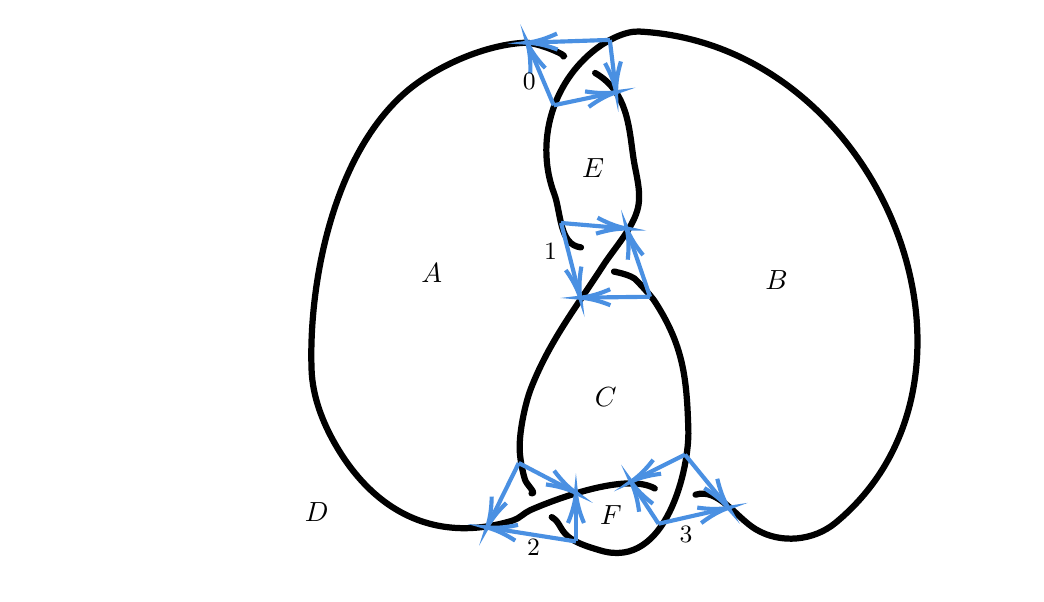
\begin{tikzpicture}[x=0.85pt,y=0.75pt,yscale=-0.9,xscale=0.9]
%uncomment if require: \path (0,877); %set diagram left start at 0, and has height of 877

%Shape: Free Drawing [id:dp052719054339937954] 
\draw  [line width=2.25] [line join = round][line cap = round] (287.39,145.57) .. controls (277.01,144.32) and (278.03,126.78) .. (274.73,116.85) .. controls (265.82,90.11) and (273.17,57.75) .. (294.63,39.17) .. controls (299.44,35.01) and (308.14,29.62) .. (314.87,30.02) .. controls (429.8,36.81) and (491.19,214.64) .. (407.67,292.97) .. controls (397.46,302.54) and (381.91,304.56) .. (369.98,296.5) .. controls (360.6,290.15) and (352.15,274.14) .. (341.49,277.97) ;
%Shape: Free Drawing [id:dp25610451731952133] 
\draw  [line width=2.25] [line join = round][line cap = round] (322.25,274.65) .. controls (309.14,266) and (275.87,280.02) .. (263.45,286.22) .. controls (260.49,287.69) and (258.35,290.7) .. (255.22,291.78) .. controls (218.11,304.6) and (189.64,286.34) .. (171.87,252.05) .. controls (165.39,239.55) and (160.62,225.56) .. (160.14,211.36) .. controls (158.61,166.54) and (169.69,97.98) .. (203.58,63.49) .. controls (217.17,49.66) and (240.46,37.41) .. (260.26,36.05) .. controls (267.59,35.55) and (282.28,43.73) .. (279.03,43.34) ;
%Shape: Free Drawing [id:dp5679641581314395] 
\draw  [line width=2.25] [line join = round][line cap = round] (294.08,52.2) .. controls (309.66,62.48) and (309.98,81.23) .. (312.22,98.19) .. controls (313.38,106.94) and (316.36,116.92) .. (313.9,126.09) .. controls (311.17,136.3) and (302.82,146.56) .. (297.8,155.38) .. controls (285.1,177.65) and (272.32,196.06) .. (263.69,221.28) .. controls (261.03,229.08) and (257.74,245.85) .. (258.53,255.91) .. controls (258.89,260.59) and (259.75,265.24) .. (260.89,269.79) .. controls (261.54,272.4) and (266.69,277.54) .. (264.02,277.22) ;
%Shape: Free Drawing [id:dp6189964124099764] 
\draw  [line width=2.25] [line join = round][line cap = round] (273.57,289.95) .. controls (278.3,293.07) and (276.89,297.76) .. (283.68,302.24) .. controls (287.6,304.83) and (292.16,306.32) .. (296.61,307.83) .. controls (327.83,318.42) and (338.62,263.49) .. (338.1,243.31) .. controls (337.37,215.47) and (335.79,198.2) .. (322.2,174.43) .. controls (320.36,171.21) and (313.27,162.71) .. (312.59,162.19) .. controls (308.57,159.15) and (299.94,158.15) .. (303.95,158.64) ;
%Shape: Free Drawing [id:dp23463200731808187] 
\draw  [color={rgb, 255:red, 255; green, 255; blue, 255 }  ,draw opacity=1 ][line width=2.25] [line join = round][line cap = round] (282.71,151.05) .. controls (282.39,151.16) and (281.67,151.26) .. (281.71,150.93) ;
%Shape: Free Drawing [id:dp6791599529562201] 
\draw  [draw opacity=0][line width=2.25] [line join = round][line cap = round] (448.19,89.85) .. controls (448.33,89.94) and (448.85,89.93) .. (448.68,89.91) ;
%Shape: Free Drawing [id:dp4292482997182422] 
\draw  [draw opacity=0][line width=2.25] [line join = round][line cap = round] (290.05,144.38) .. controls (286.7,145.58) and (285.16,148.61) .. (284.14,151.72) ;
%Shape: Free Drawing [id:dp6085326410058335] 
\draw  [draw opacity=0][line width=2.25] [line join = round][line cap = round] (288.33,146.18) .. controls (279.73,155.6) and (278.21,156.05) .. (281.06,156.39) ;
%Shape: Free Drawing [id:dp9043644710987669] 
\draw  [draw opacity=0][line width=2.25] [line join = round][line cap = round] (288.94,145.25) .. controls (286.29,148.02) and (282.99,150.44) .. (281.35,153.91) ;
%Shape: Free Drawing [id:dp21505097221297298] 
\draw  [draw opacity=0][line width=2.25] [line join = round][line cap = round] (268.43,278.25) .. controls (266.45,279.36) and (264.63,280.8) .. (262.49,281.57) .. controls (261.93,281.77) and (263.07,280.13) .. (263.67,280.2) ;
%Shape: Free Drawing [id:dp28830093222917674] 
\draw  [draw opacity=0][line width=2.25] [line join = round][line cap = round] (259.08,280.66) .. controls (262.87,278.63) and (266.13,273.95) .. (270.4,274.46) ;
%Shape: Free Drawing [id:dp9547251910894086] 
\draw  [draw opacity=0][line width=2.25] [line join = round][line cap = round] (264.4,278.27) .. controls (267.07,278.59) and (269.43,276.35) .. (271.83,275.14) ;
%Shape: Free Drawing [id:dp719981311992137] 
\draw  [draw opacity=0][line width=2.25] [line join = round][line cap = round] (262.53,277.04) .. controls (264.04,276.73) and (270.71,276.07) .. (271.01,273.53) ;
%Shape: Free Drawing [id:dp29834365303629773] 
\draw  [draw opacity=0][line width=2.25] [line join = round][line cap = round] (262.91,278.09) .. controls (265.7,276.89) and (272.86,274.94) .. (273.36,270.79) ;
%Shape: Free Drawing [id:dp42617767268148665] 
\draw  [draw opacity=0][line width=2.25] [line join = round][line cap = round] (262.79,279.09) .. controls (266.54,276.42) and (270.14,273.51) .. (273.42,270.29) ;
%Shape: Free Drawing [id:dp5503601990364082] 
\draw  [draw opacity=0][line width=2.25] [line join = round][line cap = round] (261.8,278.97) .. controls (267.65,274.97) and (271.24,270.34) .. (275.13,264.45) ;
%Shape: Free Drawing [id:dp12708063524714575] 
\draw  [draw opacity=0][line width=2.25] [line join = round][line cap = round] (29,80) .. controls (28.37,79.68) and (27.82,79.13) .. (27.5,78.5) ;
%Straight Lines [id:da7851146054141257] 
\draw [color={rgb, 255:red, 74; green, 144; blue, 226 }  ,draw opacity=1 ][line width=1.5]    (274.5,69.5) -- (301.08,63.19) ;
\draw [shift={(304,62.5)}, rotate = 166.65] [color={rgb, 255:red, 74; green, 144; blue, 226 }  ,draw opacity=1 ][line width=1.5]    (14.21,-4.28) .. controls (9.04,-1.82) and (4.3,-0.39) .. (0,0) .. controls (4.3,0.39) and (9.04,1.82) .. (14.21,4.28)   ;
%Straight Lines [id:da4904183098904815] 
\draw [color={rgb, 255:red, 74; green, 144; blue, 226 }  ,draw opacity=1 ][line width=1.5]    (274.5,69.5) -- (263.05,38.81) ;
\draw [shift={(262,36)}, rotate = 69.54] [color={rgb, 255:red, 74; green, 144; blue, 226 }  ,draw opacity=1 ][line width=1.5]    (14.21,-4.28) .. controls (9.04,-1.82) and (4.3,-0.39) .. (0,0) .. controls (4.3,0.39) and (9.04,1.82) .. (14.21,4.28)   ;
%Straight Lines [id:da21498342913887913] 
\draw [color={rgb, 255:red, 74; green, 144; blue, 226 }  ,draw opacity=1 ][line width=1.5]    (301,34.5) -- (303.68,59.52) ;
\draw [shift={(304,62.5)}, rotate = 263.88] [color={rgb, 255:red, 74; green, 144; blue, 226 }  ,draw opacity=1 ][line width=1.5]    (14.21,-4.28) .. controls (9.04,-1.82) and (4.3,-0.39) .. (0,0) .. controls (4.3,0.39) and (9.04,1.82) .. (14.21,4.28)   ;
%Straight Lines [id:da5005258690622153] 
\draw [color={rgb, 255:red, 74; green, 144; blue, 226 }  ,draw opacity=1 ][line width=1.5]    (301,34.5) -- (265,35.88) ;
\draw [shift={(262,36)}, rotate = 357.8] [color={rgb, 255:red, 74; green, 144; blue, 226 }  ,draw opacity=1 ][line width=1.5]    (14.21,-4.28) .. controls (9.04,-1.82) and (4.3,-0.39) .. (0,0) .. controls (4.3,0.39) and (9.04,1.82) .. (14.21,4.28)   ;
%Straight Lines [id:da6750405427654139] 
\draw [color={rgb, 255:red, 74; green, 144; blue, 226 }  ,draw opacity=1 ][line width=1.5]    (278,132.5) -- (286.34,169.57) ;
\draw [shift={(287,172.5)}, rotate = 257.32] [color={rgb, 255:red, 74; green, 144; blue, 226 }  ,draw opacity=1 ][line width=1.5]    (14.21,-4.28) .. controls (9.04,-1.82) and (4.3,-0.39) .. (0,0) .. controls (4.3,0.39) and (9.04,1.82) .. (14.21,4.28)   ;
%Straight Lines [id:da3934982113036074] 
\draw [color={rgb, 255:red, 74; green, 144; blue, 226 }  ,draw opacity=1 ][line width=1.5]    (278,132.5) -- (306.01,135.21) ;
\draw [shift={(309,135.5)}, rotate = 185.53] [color={rgb, 255:red, 74; green, 144; blue, 226 }  ,draw opacity=1 ][line width=1.5]    (14.21,-4.28) .. controls (9.04,-1.82) and (4.3,-0.39) .. (0,0) .. controls (4.3,0.39) and (9.04,1.82) .. (14.21,4.28)   ;
%Straight Lines [id:da8163214263178915] 
\draw [color={rgb, 255:red, 74; green, 144; blue, 226 }  ,draw opacity=1 ][line width=1.5]    (320,172) -- (290,172.45) ;
\draw [shift={(287,172.5)}, rotate = 359.13] [color={rgb, 255:red, 74; green, 144; blue, 226 }  ,draw opacity=1 ][line width=1.5]    (14.21,-4.28) .. controls (9.04,-1.82) and (4.3,-0.39) .. (0,0) .. controls (4.3,0.39) and (9.04,1.82) .. (14.21,4.28)   ;
%Straight Lines [id:da9808570839490202] 
\draw [color={rgb, 255:red, 74; green, 144; blue, 226 }  ,draw opacity=1 ][line width=1.5]    (320,172) -- (309.87,138.37) ;
\draw [shift={(309,135.5)}, rotate = 73.23] [color={rgb, 255:red, 74; green, 144; blue, 226 }  ,draw opacity=1 ][line width=1.5]    (14.21,-4.28) .. controls (9.04,-1.82) and (4.3,-0.39) .. (0,0) .. controls (4.3,0.39) and (9.04,1.82) .. (14.21,4.28)   ;
%Straight Lines [id:da9411841582233399] 
\draw [color={rgb, 255:red, 74; green, 144; blue, 226 }  ,draw opacity=1 ][line width=1.5]    (258,261) -- (244.2,292.75) ;
\draw [shift={(243,295.5)}, rotate = 293.5] [color={rgb, 255:red, 74; green, 144; blue, 226 }  ,draw opacity=1 ][line width=1.5]    (14.21,-4.28) .. controls (9.04,-1.82) and (4.3,-0.39) .. (0,0) .. controls (4.3,0.39) and (9.04,1.82) .. (14.21,4.28)   ;
%Straight Lines [id:da003586680143401688] 
\draw [color={rgb, 255:red, 74; green, 144; blue, 226 }  ,draw opacity=1 ][line width=1.5]    (285,303) -- (245.95,296.03) ;
\draw [shift={(243,295.5)}, rotate = 10.12] [color={rgb, 255:red, 74; green, 144; blue, 226 }  ,draw opacity=1 ][line width=1.5]    (14.21,-4.28) .. controls (9.04,-1.82) and (4.3,-0.39) .. (0,0) .. controls (4.3,0.39) and (9.04,1.82) .. (14.21,4.28)   ;
%Straight Lines [id:da8295997211316378] 
\draw [color={rgb, 255:red, 74; green, 144; blue, 226 }  ,draw opacity=1 ][line width=1.5]    (258,261) -- (282.42,275.47) ;
\draw [shift={(285,277)}, rotate = 210.65] [color={rgb, 255:red, 74; green, 144; blue, 226 }  ,draw opacity=1 ][line width=1.5]    (14.21,-4.28) .. controls (9.04,-1.82) and (4.3,-0.39) .. (0,0) .. controls (4.3,0.39) and (9.04,1.82) .. (14.21,4.28)   ;
%Straight Lines [id:da4207009837534177] 
\draw [color={rgb, 255:red, 74; green, 144; blue, 226 }  ,draw opacity=1 ][line width=1.5]    (285,303) -- (285,280) ;
\draw [shift={(285,277)}, rotate = 90] [color={rgb, 255:red, 74; green, 144; blue, 226 }  ,draw opacity=1 ][line width=1.5]    (14.21,-4.28) .. controls (9.04,-1.82) and (4.3,-0.39) .. (0,0) .. controls (4.3,0.39) and (9.04,1.82) .. (14.21,4.28)   ;
%Straight Lines [id:da7105295943160274] 
\draw [color={rgb, 255:red, 74; green, 144; blue, 226 }  ,draw opacity=1 ][line width=1.5]    (336.5,256.5) -- (313.61,269.52) ;
\draw [shift={(311,271)}, rotate = 330.38] [color={rgb, 255:red, 74; green, 144; blue, 226 }  ,draw opacity=1 ][line width=1.5]    (14.21,-4.28) .. controls (9.04,-1.82) and (4.3,-0.39) .. (0,0) .. controls (4.3,0.39) and (9.04,1.82) .. (14.21,4.28)   ;
%Straight Lines [id:da6405444868178161] 
\draw [color={rgb, 255:red, 74; green, 144; blue, 226 }  ,draw opacity=1 ][line width=1.5]    (324,293.5) -- (312.5,273.6) ;
\draw [shift={(311,271)}, rotate = 59.98] [color={rgb, 255:red, 74; green, 144; blue, 226 }  ,draw opacity=1 ][line width=1.5]    (14.21,-4.28) .. controls (9.04,-1.82) and (4.3,-0.39) .. (0,0) .. controls (4.3,0.39) and (9.04,1.82) .. (14.21,4.28)   ;
%Straight Lines [id:da5651565239928864] 
\draw [color={rgb, 255:red, 74; green, 144; blue, 226 }  ,draw opacity=1 ][line width=1.5]    (324,293.5) -- (354.09,285.75) ;
\draw [shift={(357,285)}, rotate = 165.56] [color={rgb, 255:red, 74; green, 144; blue, 226 }  ,draw opacity=1 ][line width=1.5]    (14.21,-4.28) .. controls (9.04,-1.82) and (4.3,-0.39) .. (0,0) .. controls (4.3,0.39) and (9.04,1.82) .. (14.21,4.28)   ;
%Straight Lines [id:da48389743721592937] 
\draw [color={rgb, 255:red, 74; green, 144; blue, 226 }  ,draw opacity=1 ][line width=1.5]    (336.5,256.5) -- (355.25,282.56) ;
\draw [shift={(357,285)}, rotate = 234.27] [color={rgb, 255:red, 74; green, 144; blue, 226 }  ,draw opacity=1 ][line width=1.5]    (14.21,-4.28) .. controls (9.04,-1.82) and (4.3,-0.39) .. (0,0) .. controls (4.3,0.39) and (9.04,1.82) .. (14.21,4.28)   ;

% Text Node
\draw (210.5,152.4) node [anchor=north west][inner sep=0.75pt]    {$A$};
% Text Node
\draw (373,156.4) node [anchor=north west][inner sep=0.75pt]    {$B$};
% Text Node
\draw (292.5,218.9) node [anchor=north west][inner sep=0.75pt]    {$C$};
% Text Node
\draw (155.5,280.4) node [anchor=north west][inner sep=0.75pt]    {$D$};
% Text Node
\draw (286.5,96.4) node [anchor=north west][inner sep=0.75pt]    {$E$};
% Text Node
\draw (295,281.9) node [anchor=north west][inner sep=0.75pt]    {$F$};
% Text Node
\draw (258.5,50.9) node [anchor=north west][inner sep=0.75pt]  [font=\small]  {$0$};
% Text Node
\draw (268.5,141.9) node [anchor=north west][inner sep=0.75pt]  [font=\small]  {$1$};
% Text Node
\draw (260.5,300.4) node [anchor=north west][inner sep=0.75pt]  [font=\small]  {$2$};
% Text Node
\draw (332.5,293.4) node [anchor=north west][inner sep=0.75pt]  [font=\small]  {$3$};


\end{tikzpicture}

\caption{Paso 1 del algoritmo para el nudo de 8}

\end{figure}
Observe que por ejemplo la cara identificada por $A$ las aristas que la rodean son la $0,1$ y $2$. lo cual en la ilustración con solo $1$ arista por cruce es bastante difícil de ver
\begin{block}
    Contraiga cada cuerda que sea un cruce superior a un punto, este punto sera el vértice ideal de nuestro poliedro superior, dado por la esfera de arriba.
\end{block}

Una observación relevante es que contraer estas cuerdas a un punto es posible ya que el complemento de un punto en $S^2$ es homeomorfo al complemento de un segmento de recta en $S^2$, esto se puede mostrar fácilmente con ayuda de la proyección estereográfica, la otra observación que es netamente de visualización es que estamos viendo el grafo desde dentro de la bola superior, esto lo haremos con un paso intermedio que se puede ver en el siguiente diagrama
\begin{figure}[H]
    \centering
    
%!TEX root = ./main.tex


\tikzset{every picture/.style={line width=0.75pt}} %set default line width to 0.75pt        

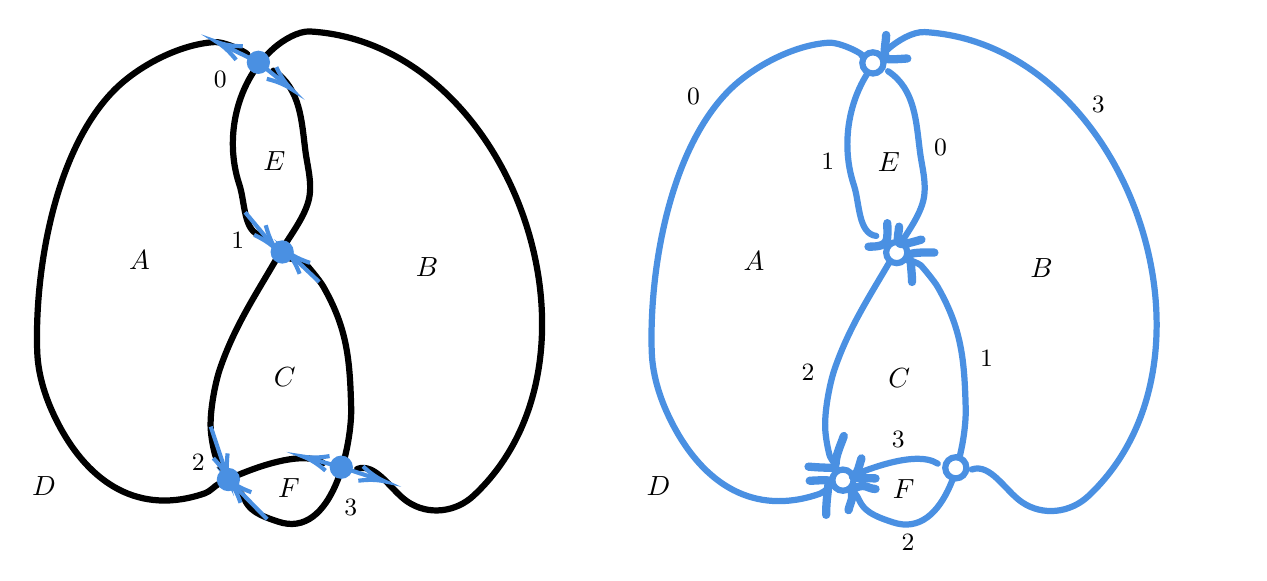
\begin{tikzpicture}[x=0.75pt,y=0.75pt,yscale=-0.85,xscale=0.85]
%uncomment if require: \path (0,877); %set diagram left start at 0, and has height of 877

%Shape: Free Drawing [id:dp052719054339937954] 
\draw  [line width=2.25] [line join = round][line cap = round] (144.39,147.9) .. controls (134.01,146.65) and (135.03,129.11) .. (131.73,119.19) .. controls (122.82,92.44) and (130.17,60.08) .. (151.63,41.51) .. controls (156.44,37.34) and (165.14,31.96) .. (171.87,32.35) .. controls (286.8,39.15) and (348.19,216.97) .. (264.67,295.3) .. controls (254.46,304.88) and (238.91,306.9) .. (226.98,298.83) .. controls (217.6,292.48) and (209.15,276.48) .. (198.49,280.3) ;
%Shape: Free Drawing [id:dp25610451731952133] 
\draw  [line width=2.25] [line join = round][line cap = round] (179.25,276.98) .. controls (166.14,268.33) and (132.87,282.35) .. (120.45,288.55) .. controls (117.49,290.03) and (115.35,293.03) .. (112.22,294.11) .. controls (75.11,306.93) and (46.64,288.67) .. (28.87,254.38) .. controls (22.39,241.88) and (17.62,227.89) .. (17.14,213.69) .. controls (15.61,168.88) and (26.69,100.32) .. (60.58,65.82) .. controls (74.17,52) and (97.46,39.75) .. (117.26,38.38) .. controls (124.59,37.88) and (139.28,46.06) .. (136.03,45.67) ;
%Shape: Free Drawing [id:dp5679641581314395] 
\draw  [line width=2.25] [line join = round][line cap = round] (151.08,54.53) .. controls (166.66,64.82) and (166.98,83.56) .. (169.22,100.52) .. controls (170.38,109.27) and (173.36,119.25) .. (170.9,128.42) .. controls (168.17,138.64) and (159.82,148.9) .. (154.8,157.71) .. controls (142.1,179.99) and (129.32,198.39) .. (120.69,223.62) .. controls (118.03,231.41) and (114.74,248.18) .. (115.53,258.25) .. controls (115.89,262.93) and (116.75,267.57) .. (117.89,272.13) .. controls (118.54,274.73) and (123.69,279.87) .. (121.02,279.55) ;
%Shape: Free Drawing [id:dp6189964124099764] 
\draw  [line width=2.25] [line join = round][line cap = round] (130.57,292.28) .. controls (135.3,295.4) and (133.89,300.1) .. (140.68,304.58) .. controls (144.6,307.16) and (149.16,308.65) .. (153.61,310.16) .. controls (184.83,320.75) and (195.62,265.82) .. (195.1,245.65) .. controls (194.37,217.8) and (192.79,200.53) .. (179.2,176.76) .. controls (177.36,173.55) and (170.27,165.04) .. (169.59,164.53) .. controls (165.57,161.48) and (156.94,160.49) .. (160.95,160.97) ;
%Shape: Free Drawing [id:dp23463200731808187] 
\draw  [color={rgb, 255:red, 255; green, 255; blue, 255 }  ,draw opacity=1 ][line width=2.25] [line join = round][line cap = round] (139.71,153.38) .. controls (139.39,153.49) and (138.67,153.59) .. (138.71,153.26) ;
%Shape: Free Drawing [id:dp6791599529562201] 
\draw  [draw opacity=0][line width=2.25] [line join = round][line cap = round] (305.19,92.18) .. controls (305.33,92.27) and (305.85,92.26) .. (305.68,92.24) ;
%Shape: Free Drawing [id:dp4292482997182422] 
\draw  [draw opacity=0][line width=2.25] [line join = round][line cap = round] (147.05,146.71) .. controls (143.7,147.91) and (142.16,150.95) .. (141.14,154.06) ;
%Shape: Free Drawing [id:dp6085326410058335] 
\draw  [draw opacity=0][line width=2.25] [line join = round][line cap = round] (145.33,148.52) .. controls (136.73,157.93) and (135.21,158.38) .. (138.06,158.72) ;
%Shape: Free Drawing [id:dp9043644710987669] 
\draw  [draw opacity=0][line width=2.25] [line join = round][line cap = round] (145.94,147.58) .. controls (143.29,150.36) and (139.99,152.77) .. (138.35,156.24) ;
%Shape: Free Drawing [id:dp21505097221297298] 
\draw  [draw opacity=0][line width=2.25] [line join = round][line cap = round] (125.43,280.59) .. controls (123.45,281.69) and (121.63,283.14) .. (119.49,283.9) .. controls (118.93,284.11) and (120.07,282.46) .. (120.67,282.53) ;
%Shape: Free Drawing [id:dp28830093222917674] 
\draw  [draw opacity=0][line width=2.25] [line join = round][line cap = round] (116.08,282.99) .. controls (119.87,280.96) and (123.13,276.28) .. (127.4,276.79) ;
%Shape: Free Drawing [id:dp9547251910894086] 
\draw  [draw opacity=0][line width=2.25] [line join = round][line cap = round] (121.4,280.61) .. controls (124.07,280.93) and (126.43,278.68) .. (128.83,277.47) ;
%Shape: Free Drawing [id:dp719981311992137] 
\draw  [draw opacity=0][line width=2.25] [line join = round][line cap = round] (119.53,279.38) .. controls (121.04,279.07) and (127.71,278.4) .. (128.01,275.86) ;
%Shape: Free Drawing [id:dp29834365303629773] 
\draw  [draw opacity=0][line width=2.25] [line join = round][line cap = round] (119.91,280.43) .. controls (122.7,279.22) and (129.86,277.27) .. (130.36,273.12) ;
%Shape: Free Drawing [id:dp42617767268148665] 
\draw  [draw opacity=0][line width=2.25] [line join = round][line cap = round] (119.79,281.42) .. controls (123.54,278.76) and (127.14,275.85) .. (130.42,272.63) ;
%Shape: Free Drawing [id:dp5503601990364082] 
\draw  [draw opacity=0][line width=2.25] [line join = round][line cap = round] (118.8,281.3) .. controls (124.65,277.3) and (128.24,272.67) .. (132.13,266.79) ;
%Shape: Free Drawing [id:dp12708063524714575] 
\draw  [draw opacity=0][line width=2.25] [line join = round][line cap = round] (15,81.33) .. controls (14.37,81.02) and (13.82,80.47) .. (13.5,79.83) ;
%Straight Lines [id:da4904183098904815] 
\draw [color={rgb, 255:red, 74; green, 144; blue, 226 }  ,draw opacity=1 ][line width=1.5]    (142.5,49.83) -- (121.69,39.65) ;
\draw [shift={(119,38.33)}, rotate = 26.08] [color={rgb, 255:red, 74; green, 144; blue, 226 }  ,draw opacity=1 ][line width=1.5]    (14.21,-4.28) .. controls (9.04,-1.82) and (4.3,-0.39) .. (0,0) .. controls (4.3,0.39) and (9.04,1.82) .. (14.21,4.28)   ;
%Straight Lines [id:da21498342913887913] 
\draw [color={rgb, 255:red, 74; green, 144; blue, 226 }  ,draw opacity=1 ][line width=1.5]    (142.5,49.83) -- (158.67,62.94) ;
\draw [shift={(161,64.83)}, rotate = 219.04] [color={rgb, 255:red, 74; green, 144; blue, 226 }  ,draw opacity=1 ][line width=1.5]    (14.21,-4.28) .. controls (9.04,-1.82) and (4.3,-0.39) .. (0,0) .. controls (4.3,0.39) and (9.04,1.82) .. (14.21,4.28)   ;
%Straight Lines [id:da6750405427654139] 
\draw [color={rgb, 255:red, 74; green, 144; blue, 226 }  ,draw opacity=1 ][line width=1.5]    (135,134.83) -- (150.58,153.53) ;
\draw [shift={(152.5,155.83)}, rotate = 230.19] [color={rgb, 255:red, 74; green, 144; blue, 226 }  ,draw opacity=1 ][line width=1.5]    (14.21,-4.28) .. controls (9.04,-1.82) and (4.3,-0.39) .. (0,0) .. controls (4.3,0.39) and (9.04,1.82) .. (14.21,4.28)   ;
%Straight Lines [id:da9808570839490202] 
\draw [color={rgb, 255:red, 74; green, 144; blue, 226 }  ,draw opacity=1 ][line width=1.5]    (177,174.33) -- (160.68,158.89) ;
\draw [shift={(158.5,156.83)}, rotate = 43.41] [color={rgb, 255:red, 74; green, 144; blue, 226 }  ,draw opacity=1 ][line width=1.5]    (14.21,-4.28) .. controls (9.04,-1.82) and (4.3,-0.39) .. (0,0) .. controls (4.3,0.39) and (9.04,1.82) .. (14.21,4.28)   ;
%Straight Lines [id:da8295997211316378] 
\draw [color={rgb, 255:red, 74; green, 144; blue, 226 }  ,draw opacity=1 ][line width=1.5]    (115.5,256.33) -- (124.55,283.49) ;
\draw [shift={(125.5,286.33)}, rotate = 251.57] [color={rgb, 255:red, 74; green, 144; blue, 226 }  ,draw opacity=1 ][line width=1.5]    (14.21,-4.28) .. controls (9.04,-1.82) and (4.3,-0.39) .. (0,0) .. controls (4.3,0.39) and (9.04,1.82) .. (14.21,4.28)   ;
%Straight Lines [id:da4207009837534177] 
\draw [color={rgb, 255:red, 74; green, 144; blue, 226 }  ,draw opacity=1 ][line width=1.5]    (147.5,308.83) -- (127.6,288.48) ;
\draw [shift={(125.5,286.33)}, rotate = 45.64] [color={rgb, 255:red, 74; green, 144; blue, 226 }  ,draw opacity=1 ][line width=1.5]    (14.21,-4.28) .. controls (9.04,-1.82) and (4.3,-0.39) .. (0,0) .. controls (4.3,0.39) and (9.04,1.82) .. (14.21,4.28)   ;
%Straight Lines [id:da7105295943160274] 
\draw [color={rgb, 255:red, 74; green, 144; blue, 226 }  ,draw opacity=1 ][line width=1.5]    (189.5,279.33) -- (170.89,274.14) ;
\draw [shift={(168,273.33)}, rotate = 15.59] [color={rgb, 255:red, 74; green, 144; blue, 226 }  ,draw opacity=1 ][line width=1.5]    (14.21,-4.28) .. controls (9.04,-1.82) and (4.3,-0.39) .. (0,0) .. controls (4.3,0.39) and (9.04,1.82) .. (14.21,4.28)   ;
%Straight Lines [id:da5651565239928864] 
\draw [color={rgb, 255:red, 74; green, 144; blue, 226 }  ,draw opacity=1 ][line width=1.5]    (189.5,279.33) -- (211.15,286.4) ;
\draw [shift={(214,287.33)}, rotate = 198.08] [color={rgb, 255:red, 74; green, 144; blue, 226 }  ,draw opacity=1 ][line width=1.5]    (14.21,-4.28) .. controls (9.04,-1.82) and (4.3,-0.39) .. (0,0) .. controls (4.3,0.39) and (9.04,1.82) .. (14.21,4.28)   ;
%Shape: Circle [id:dp7563944317650207] 
\draw  [color={rgb, 255:red, 74; green, 144; blue, 226 }  ,draw opacity=1 ][fill={rgb, 255:red, 74; green, 144; blue, 226 }  ,fill opacity=1 ] (136.5,49.83) .. controls (136.5,46.52) and (139.19,43.83) .. (142.5,43.83) .. controls (145.81,43.83) and (148.5,46.52) .. (148.5,49.83) .. controls (148.5,53.15) and (145.81,55.83) .. (142.5,55.83) .. controls (139.19,55.83) and (136.5,53.15) .. (136.5,49.83) -- cycle ;
%Shape: Circle [id:dp8058641002050105] 
\draw  [color={rgb, 255:red, 74; green, 144; blue, 226 }  ,draw opacity=1 ][fill={rgb, 255:red, 74; green, 144; blue, 226 }  ,fill opacity=1 ] (150,157.33) .. controls (150,154.02) and (152.69,151.33) .. (156,151.33) .. controls (159.31,151.33) and (162,154.02) .. (162,157.33) .. controls (162,160.65) and (159.31,163.33) .. (156,163.33) .. controls (152.69,163.33) and (150,160.65) .. (150,157.33) -- cycle ;
%Shape: Circle [id:dp3830896703653248] 
\draw  [color={rgb, 255:red, 74; green, 144; blue, 226 }  ,draw opacity=1 ][fill={rgb, 255:red, 74; green, 144; blue, 226 }  ,fill opacity=1 ] (119.5,286.33) .. controls (119.5,283.02) and (122.19,280.33) .. (125.5,280.33) .. controls (128.81,280.33) and (131.5,283.02) .. (131.5,286.33) .. controls (131.5,289.65) and (128.81,292.33) .. (125.5,292.33) .. controls (122.19,292.33) and (119.5,289.65) .. (119.5,286.33) -- cycle ;
%Shape: Circle [id:dp568354357328672] 
\draw  [color={rgb, 255:red, 74; green, 144; blue, 226 }  ,draw opacity=1 ][fill={rgb, 255:red, 74; green, 144; blue, 226 }  ,fill opacity=1 ] (183.5,279.33) .. controls (183.5,276.02) and (186.19,273.33) .. (189.5,273.33) .. controls (192.81,273.33) and (195.5,276.02) .. (195.5,279.33) .. controls (195.5,282.65) and (192.81,285.33) .. (189.5,285.33) .. controls (186.19,285.33) and (183.5,282.65) .. (183.5,279.33) -- cycle ;
%Shape: Free Drawing [id:dp4081098483122335] 
\draw  [color={rgb, 255:red, 74; green, 144; blue, 226 }  ,draw opacity=1 ][line width=2.25] [line join = round][line cap = round] (492.73,148.24) .. controls (482.34,146.99) and (483.37,129.44) .. (480.06,119.52) .. controls (471.15,92.78) and (478.5,60.42) .. (499.97,41.84) .. controls (504.78,37.68) and (513.47,32.29) .. (520.2,32.69) .. controls (635.13,39.48) and (696.52,217.31) .. (613,295.63) .. controls (602.79,305.21) and (587.24,307.23) .. (575.31,299.16) .. controls (565.93,292.82) and (557.49,276.81) .. (546.82,280.63) ;
%Shape: Free Drawing [id:dp3946430254773102] 
\draw  [color={rgb, 255:red, 74; green, 144; blue, 226 }  ,draw opacity=1 ][line width=2.25] [line join = round][line cap = round] (527.58,277.31) .. controls (514.47,268.66) and (481.2,282.69) .. (468.78,288.88) .. controls (465.82,290.36) and (463.69,293.36) .. (460.56,294.44) .. controls (423.44,307.26) and (394.97,289.01) .. (377.2,254.72) .. controls (370.72,242.22) and (365.96,228.23) .. (365.47,214.03) .. controls (363.94,169.21) and (375.02,100.65) .. (408.92,66.15) .. controls (422.5,52.33) and (445.8,40.08) .. (465.59,38.72) .. controls (472.93,38.21) and (487.61,46.4) .. (484.36,46.01) ;
%Shape: Free Drawing [id:dp031095390456670646] 
\draw  [color={rgb, 255:red, 74; green, 144; blue, 226 }  ,draw opacity=1 ][line width=2.25] [line join = round][line cap = round] (499.41,54.87) .. controls (515,65.15) and (515.31,83.9) .. (517.55,100.86) .. controls (518.71,109.6) and (521.69,119.59) .. (519.24,128.76) .. controls (516.51,138.97) and (508.15,149.23) .. (503.13,158.05) .. controls (490.43,180.32) and (477.65,198.73) .. (469.03,223.95) .. controls (466.36,231.74) and (463.07,248.52) .. (463.86,258.58) .. controls (464.22,263.26) and (465.08,267.91) .. (466.22,272.46) .. controls (466.87,275.07) and (472.03,280.21) .. (469.36,279.89) ;
%Shape: Free Drawing [id:dp4420640700184618] 
\draw  [color={rgb, 255:red, 74; green, 144; blue, 226 }  ,draw opacity=1 ][line width=2.25] [line join = round][line cap = round] (478.91,292.62) .. controls (483.63,295.74) and (482.22,300.43) .. (489.01,304.91) .. controls (492.93,307.5) and (497.49,308.98) .. (501.94,310.49) .. controls (533.16,321.08) and (543.96,266.15) .. (543.43,245.98) .. controls (542.7,218.14) and (541.13,200.87) .. (527.53,177.09) .. controls (525.7,173.88) and (518.6,165.37) .. (517.92,164.86) .. controls (513.9,161.81) and (505.27,160.82) .. (509.29,161.3) ;
%Shape: Free Drawing [id:dp7555303909696401] 
\draw  [color={rgb, 255:red, 255; green, 255; blue, 255 }  ,draw opacity=1 ][line width=2.25] [line join = round][line cap = round] (488.04,153.72) .. controls (487.73,153.83) and (487.01,153.93) .. (487.05,153.6) ;
%Shape: Free Drawing [id:dp37169312634770046] 
\draw  [draw opacity=0][line width=2.25] [line join = round][line cap = round] (653.52,92.52) .. controls (653.66,92.61) and (654.18,92.59) .. (654.02,92.57) ;
%Shape: Free Drawing [id:dp9746607410675733] 
\draw  [draw opacity=0][line width=2.25] [line join = round][line cap = round] (495.39,147.04) .. controls (492.03,148.25) and (490.49,151.28) .. (489.47,154.39) ;
%Shape: Free Drawing [id:dp1538069765158795] 
\draw  [draw opacity=0][line width=2.25] [line join = round][line cap = round] (493.66,148.85) .. controls (485.06,158.27) and (483.54,158.71) .. (486.39,159.06) ;
%Shape: Free Drawing [id:dp7648430884866061] 
\draw  [draw opacity=0][line width=2.25] [line join = round][line cap = round] (494.27,147.92) .. controls (491.62,150.69) and (488.33,153.11) .. (486.69,156.57) ;
%Shape: Free Drawing [id:dp06814306363407108] 
\draw  [draw opacity=0][line width=2.25] [line join = round][line cap = round] (473.77,280.92) .. controls (471.79,282.03) and (469.96,283.47) .. (467.83,284.24) .. controls (467.26,284.44) and (468.4,282.79) .. (469,282.87) ;
%Shape: Free Drawing [id:dp9432314319008595] 
\draw  [draw opacity=0][line width=2.25] [line join = round][line cap = round] (464.41,283.32) .. controls (468.2,281.29) and (471.46,276.62) .. (475.73,277.13) ;
%Shape: Free Drawing [id:dp868875743192955] 
\draw  [draw opacity=0][line width=2.25] [line join = round][line cap = round] (469.73,280.94) .. controls (472.4,281.26) and (474.76,279.02) .. (477.16,277.8) ;
%Shape: Free Drawing [id:dp38260252168946307] 
\draw  [draw opacity=0][line width=2.25] [line join = round][line cap = round] (467.87,279.71) .. controls (469.37,279.4) and (476.04,278.73) .. (476.35,276.19) ;
%Shape: Free Drawing [id:dp16315732791425064] 
\draw  [draw opacity=0][line width=2.25] [line join = round][line cap = round] (468.24,280.76) .. controls (471.04,279.55) and (478.19,277.6) .. (478.69,273.45) ;
%Shape: Free Drawing [id:dp9749908385719288] 
\draw  [draw opacity=0][line width=2.25] [line join = round][line cap = round] (468.13,281.75) .. controls (471.87,279.09) and (475.47,276.18) .. (478.75,272.96) ;
%Shape: Free Drawing [id:dp34001164497982994] 
\draw  [draw opacity=0][line width=2.25] [line join = round][line cap = round] (467.13,281.63) .. controls (472.99,277.64) and (476.58,273.01) .. (480.46,267.12) ;
%Shape: Circle [id:dp954115660091245] 
\draw  [color={rgb, 255:red, 74; green, 144; blue, 226 }  ,draw opacity=1 ][fill={rgb, 255:red, 255; green, 255; blue, 255 }  ,fill opacity=1 ][line width=2.25]  (484.83,50.17) .. controls (484.83,46.85) and (487.52,44.17) .. (490.83,44.17) .. controls (494.15,44.17) and (496.83,46.85) .. (496.83,50.17) .. controls (496.83,53.48) and (494.15,56.17) .. (490.83,56.17) .. controls (487.52,56.17) and (484.83,53.48) .. (484.83,50.17) -- cycle ;
%Shape: Circle [id:dp12690402095779774] 
\draw  [color={rgb, 255:red, 74; green, 144; blue, 226 }  ,draw opacity=1 ][fill={rgb, 255:red, 74; green, 144; blue, 226 }  ,fill opacity=1 ] (498.33,157.67) .. controls (498.33,154.35) and (501.02,151.67) .. (504.33,151.67) .. controls (507.65,151.67) and (510.33,154.35) .. (510.33,157.67) .. controls (510.33,160.98) and (507.65,163.67) .. (504.33,163.67) .. controls (501.02,163.67) and (498.33,160.98) .. (498.33,157.67) -- cycle ;
%Shape: Circle [id:dp06506143308802792] 
\draw  [color={rgb, 255:red, 74; green, 144; blue, 226 }  ,draw opacity=1 ][fill={rgb, 255:red, 74; green, 144; blue, 226 }  ,fill opacity=1 ] (467.83,286.67) .. controls (467.83,283.35) and (470.52,280.67) .. (473.83,280.67) .. controls (477.15,280.67) and (479.83,283.35) .. (479.83,286.67) .. controls (479.83,289.98) and (477.15,292.67) .. (473.83,292.67) .. controls (470.52,292.67) and (467.83,289.98) .. (467.83,286.67) -- cycle ;
%Shape: Circle [id:dp9939141058309052] 
\draw  [color={rgb, 255:red, 74; green, 144; blue, 226 }  ,draw opacity=1 ][fill={rgb, 255:red, 74; green, 144; blue, 226 }  ,fill opacity=1 ] (531.83,279.67) .. controls (531.83,276.35) and (534.52,273.67) .. (537.83,273.67) .. controls (541.15,273.67) and (543.83,276.35) .. (543.83,279.67) .. controls (543.83,282.98) and (541.15,285.67) .. (537.83,285.67) .. controls (534.52,285.67) and (531.83,282.98) .. (531.83,279.67) -- cycle ;
%Shape: Circle [id:dp006791002980818472] 
\draw  [color={rgb, 255:red, 74; green, 144; blue, 226 }  ,draw opacity=1 ][fill={rgb, 255:red, 255; green, 255; blue, 255 }  ,fill opacity=1 ][line width=2.25]  (498.33,157.67) .. controls (498.33,154.35) and (501.02,151.67) .. (504.33,151.67) .. controls (507.65,151.67) and (510.33,154.35) .. (510.33,157.67) .. controls (510.33,160.98) and (507.65,163.67) .. (504.33,163.67) .. controls (501.02,163.67) and (498.33,160.98) .. (498.33,157.67) -- cycle ;
%Shape: Circle [id:dp919820840892326] 
\draw  [color={rgb, 255:red, 74; green, 144; blue, 226 }  ,draw opacity=1 ][fill={rgb, 255:red, 255; green, 255; blue, 255 }  ,fill opacity=1 ][line width=2.25]  (467.83,286.67) .. controls (467.83,283.35) and (470.52,280.67) .. (473.83,280.67) .. controls (477.15,280.67) and (479.83,283.35) .. (479.83,286.67) .. controls (479.83,289.98) and (477.15,292.67) .. (473.83,292.67) .. controls (470.52,292.67) and (467.83,289.98) .. (467.83,286.67) -- cycle ;
%Shape: Circle [id:dp5154014024748038] 
\draw  [color={rgb, 255:red, 74; green, 144; blue, 226 }  ,draw opacity=1 ][fill={rgb, 255:red, 255; green, 255; blue, 255 }  ,fill opacity=1 ][line width=2.25]  (531.83,279.67) .. controls (531.83,276.35) and (534.52,273.67) .. (537.83,273.67) .. controls (541.15,273.67) and (543.83,276.35) .. (543.83,279.67) .. controls (543.83,282.98) and (541.15,285.67) .. (537.83,285.67) .. controls (534.52,285.67) and (531.83,282.98) .. (531.83,279.67) -- cycle ;
%Shape: Free Drawing [id:dp7512942112724584] 
\draw  [color={rgb, 255:red, 74; green, 144; blue, 226 }  ,draw opacity=1 ][line width=3] [line join = round][line cap = round] (469,279.67) .. controls (464.11,279.67) and (459.21,279.44) .. (454.33,279) ;
%Shape: Free Drawing [id:dp34845684588155923] 
\draw  [color={rgb, 255:red, 74; green, 144; blue, 226 }  ,draw opacity=1 ][line width=3] [line join = round][line cap = round] (469.67,277.67) .. controls (469.67,272.56) and (472.73,266.46) .. (474.33,261.67) ;
%Shape: Free Drawing [id:dp6085374109120528] 
\draw  [color={rgb, 255:red, 74; green, 144; blue, 226 }  ,draw opacity=1 ][line width=3] [line join = round][line cap = round] (484.33,274.33) .. controls (483.44,277) and (482.92,279.82) .. (481.67,282.33) .. controls (481.17,283.33) and (478.63,284.61) .. (479.67,285) .. controls (480.71,285.39) and (490.91,285.67) .. (492.33,285.67) ;
%Shape: Free Drawing [id:dp7749044227211802] 
\draw  [color={rgb, 255:red, 74; green, 144; blue, 226 }  ,draw opacity=1 ][line width=3] [line join = round][line cap = round] (455,287) .. controls (459,287) and (463.06,286.3) .. (467,287) .. controls (467.79,287.14) and (465.76,288.2) .. (465.67,289) .. controls (464.82,296.64) and (464.33,299.97) .. (464.33,306.33) ;
%Shape: Free Drawing [id:dp10346459869848679] 
\draw  [color={rgb, 255:red, 74; green, 144; blue, 226 }  ,draw opacity=1 ][line width=3] [line join = round][line cap = round] (477,303.67) .. controls (477.46,301.39) and (478.44,299.25) .. (479,297) .. controls (479.43,295.26) and (478.11,292.55) .. (479.67,291.67) .. controls (486.4,287.88) and (487.85,291.67) .. (492.33,291.67) ;
%Shape: Free Drawing [id:dp9094306621747547] 
\draw  [color={rgb, 255:red, 74; green, 144; blue, 226 }  ,draw opacity=1 ][line width=3] [line join = round][line cap = round] (498.33,34.33) .. controls (498.33,38.78) and (496.58,43.58) .. (498.33,47.67) .. controls (498.76,48.66) and (509.78,47.67) .. (510.33,47.67) ;
%Shape: Free Drawing [id:dp9371550972142336] 
\draw  [color={rgb, 255:red, 74; green, 144; blue, 226 }  ,draw opacity=1 ][line width=3] [line join = round][line cap = round] (505.67,143) .. controls (505.67,146.11) and (503.98,149.72) .. (505.67,152.33) .. controls (506.77,154.06) and (518.03,150.33) .. (518.33,150.33) ;
%Shape: Free Drawing [id:dp16012343838757115] 
\draw  [color={rgb, 255:red, 74; green, 144; blue, 226 }  ,draw opacity=1 ][line width=3] [line join = round][line cap = round] (488.33,154.33) .. controls (500.55,154.33) and (499,151.21) .. (499,141) ;
%Shape: Free Drawing [id:dp9681856106265141] 
\draw  [color={rgb, 255:red, 74; green, 144; blue, 226 }  ,draw opacity=1 ][line width=3] [line join = round][line cap = round] (525.67,157.67) .. controls (522.88,157.67) and (513.67,157.22) .. (511,159) .. controls (509.65,159.9) and (512.23,162.05) .. (512.33,163.67) .. controls (512.57,167.22) and (513,170.77) .. (513,174.33) ;

% Text Node
\draw (67.5,154.73) node [anchor=north west][inner sep=0.75pt]    {$A$};
% Text Node
\draw (230,158.73) node [anchor=north west][inner sep=0.75pt]    {$B$};
% Text Node
\draw (149.5,221.23) node [anchor=north west][inner sep=0.75pt]    {$C$};
% Text Node
\draw (12.5,282.73) node [anchor=north west][inner sep=0.75pt]    {$D$};
% Text Node
\draw (143.5,98.73) node [anchor=north west][inner sep=0.75pt]    {$E$};
% Text Node
\draw (152,284.23) node [anchor=north west][inner sep=0.75pt]    {$F$};
% Text Node
\draw (115.5,53.23) node [anchor=north west][inner sep=0.75pt]  [font=\small]  {$0$};
% Text Node
\draw (125.5,144.23) node [anchor=north west][inner sep=0.75pt]  [font=\small]  {$1$};
% Text Node
\draw (103,270.23) node [anchor=north west][inner sep=0.75pt]  [font=\small]  {$2$};
% Text Node
\draw (189.5,295.73) node [anchor=north west][inner sep=0.75pt]  [font=\small]  {$3$};
% Text Node
\draw (415.83,155.07) node [anchor=north west][inner sep=0.75pt]    {$A$};
% Text Node
\draw (578.33,159.07) node [anchor=north west][inner sep=0.75pt]    {$B$};
% Text Node
\draw (497.83,221.57) node [anchor=north west][inner sep=0.75pt]    {$C$};
% Text Node
\draw (360.83,283.07) node [anchor=north west][inner sep=0.75pt]    {$D$};
% Text Node
\draw (491.83,99.07) node [anchor=north west][inner sep=0.75pt]    {$E$};
% Text Node
\draw (500.33,284.57) node [anchor=north west][inner sep=0.75pt]    {$F$};
% Text Node
\draw (383.83,62.9) node [anchor=north west][inner sep=0.75pt]  [font=\small]  {$0$};
% Text Node
\draw (459.83,99.9) node [anchor=north west][inner sep=0.75pt]  [font=\small]  {$1$};
% Text Node
\draw (448.67,219.23) node [anchor=north west][inner sep=0.75pt]  [font=\small]  {$2$};
% Text Node
\draw (499.83,257.4) node [anchor=north west][inner sep=0.75pt]  [font=\small]  {$3$};
% Text Node
\draw (549.83,211.23) node [anchor=north west][inner sep=0.75pt]  [font=\small]  {$1$};
% Text Node
\draw (523.83,91.57) node [anchor=north west][inner sep=0.75pt]  [font=\small]  {$0$};
% Text Node
\draw (505.33,315.9) node [anchor=north west][inner sep=0.75pt]  [font=\small]  {$2$};
% Text Node
\draw (613.17,67.4) node [anchor=north west][inner sep=0.75pt]  [font=\small]  {$3$};


\end{tikzpicture}

    \caption{Paso intermedio y paso 2 para el nudo de 8}
\end{figure}
\begin{block}
    De manera similar a antes contraiga ahora cada cruce por debajo como si fuera una cuerda continua a un punto, estos serán los vértices ideales del poliedro inferior, dado por la esfera de abajo.
\end{block}
Observe que para el poliedro de abajo lo que para nosotros desde el diagrama es una cuerda que pasa por debajo, para este sera una cuerda que pasa por encima, por eso ahora contraemos los cruces así
\begin{figure}[H]
    \centering
    
%!TEX root = ./main.tex



\tikzset{every picture/.style={line width=0.75pt}} %set default line width to 0.75pt        

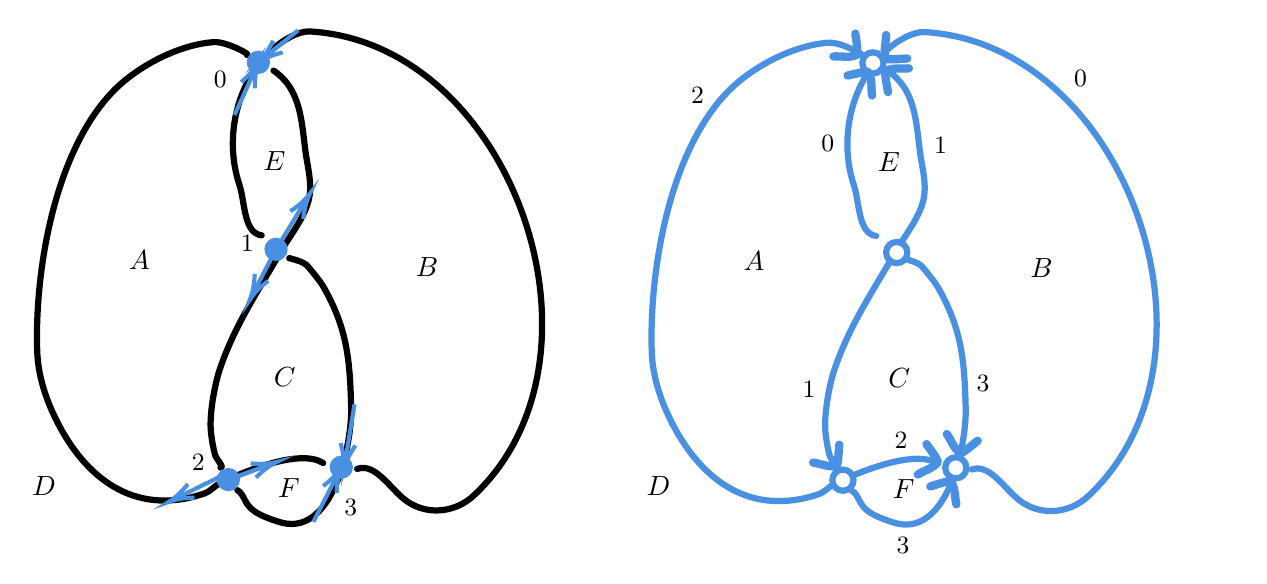
\begin{tikzpicture}[x=0.75pt,y=0.75pt,yscale=-0.85,xscale=0.85]
%uncomment if require: \path (0,877); %set diagram left start at 0, and has height of 877

%Shape: Free Drawing [id:dp052719054339937954] 
\draw  [line width=2.25] [line join = round][line cap = round] (144.39,147.9) .. controls (134.01,146.65) and (135.03,129.11) .. (131.73,119.19) .. controls (122.82,92.44) and (130.17,60.08) .. (151.63,41.51) .. controls (156.44,37.34) and (165.14,31.96) .. (171.87,32.35) .. controls (286.8,39.15) and (348.19,216.97) .. (264.67,295.3) .. controls (254.46,304.88) and (238.91,306.9) .. (226.98,298.83) .. controls (217.6,292.48) and (209.15,276.48) .. (198.49,280.3) ;
%Shape: Free Drawing [id:dp25610451731952133] 
\draw  [line width=2.25] [line join = round][line cap = round] (179.25,276.98) .. controls (166.14,268.33) and (132.87,282.35) .. (120.45,288.55) .. controls (117.49,290.03) and (115.35,293.03) .. (112.22,294.11) .. controls (75.11,306.93) and (46.64,288.67) .. (28.87,254.38) .. controls (22.39,241.88) and (17.62,227.89) .. (17.14,213.69) .. controls (15.61,168.88) and (26.69,100.32) .. (60.58,65.82) .. controls (74.17,52) and (97.46,39.75) .. (117.26,38.38) .. controls (124.59,37.88) and (139.28,46.06) .. (136.03,45.67) ;
%Shape: Free Drawing [id:dp5679641581314395] 
\draw  [line width=2.25] [line join = round][line cap = round] (151.08,54.53) .. controls (166.66,64.82) and (166.98,83.56) .. (169.22,100.52) .. controls (170.38,109.27) and (173.36,119.25) .. (170.9,128.42) .. controls (168.17,138.64) and (159.82,148.9) .. (154.8,157.71) .. controls (142.1,179.99) and (129.32,198.39) .. (120.69,223.62) .. controls (118.03,231.41) and (114.74,248.18) .. (115.53,258.25) .. controls (115.89,262.93) and (116.75,267.57) .. (117.89,272.13) .. controls (118.54,274.73) and (123.69,279.87) .. (121.02,279.55) ;
%Shape: Free Drawing [id:dp6189964124099764] 
\draw  [line width=2.25] [line join = round][line cap = round] (130.57,292.28) .. controls (135.3,295.4) and (133.89,300.1) .. (140.68,304.58) .. controls (144.6,307.16) and (149.16,308.65) .. (153.61,310.16) .. controls (184.83,320.75) and (195.62,265.82) .. (195.1,245.65) .. controls (194.37,217.8) and (192.79,200.53) .. (179.2,176.76) .. controls (177.36,173.55) and (170.27,165.04) .. (169.59,164.53) .. controls (165.57,161.48) and (156.94,160.49) .. (160.95,160.97) ;
%Shape: Free Drawing [id:dp23463200731808187] 
\draw  [color={rgb, 255:red, 255; green, 255; blue, 255 }  ,draw opacity=1 ][line width=2.25] [line join = round][line cap = round] (139.71,153.38) .. controls (139.39,153.49) and (138.67,153.59) .. (138.71,153.26) ;
%Shape: Free Drawing [id:dp6791599529562201] 
\draw  [draw opacity=0][line width=2.25] [line join = round][line cap = round] (305.19,92.18) .. controls (305.33,92.27) and (305.85,92.26) .. (305.68,92.24) ;
%Shape: Free Drawing [id:dp4292482997182422] 
\draw  [draw opacity=0][line width=2.25] [line join = round][line cap = round] (147.05,146.71) .. controls (143.7,147.91) and (142.16,150.95) .. (141.14,154.06) ;
%Shape: Free Drawing [id:dp6085326410058335] 
\draw  [draw opacity=0][line width=2.25] [line join = round][line cap = round] (145.33,148.52) .. controls (136.73,157.93) and (135.21,158.38) .. (138.06,158.72) ;
%Shape: Free Drawing [id:dp9043644710987669] 
\draw  [draw opacity=0][line width=2.25] [line join = round][line cap = round] (145.94,147.58) .. controls (143.29,150.36) and (139.99,152.77) .. (138.35,156.24) ;
%Shape: Free Drawing [id:dp21505097221297298] 
\draw  [draw opacity=0][line width=2.25] [line join = round][line cap = round] (125.43,280.59) .. controls (123.45,281.69) and (121.63,283.14) .. (119.49,283.9) .. controls (118.93,284.11) and (120.07,282.46) .. (120.67,282.53) ;
%Shape: Free Drawing [id:dp28830093222917674] 
\draw  [draw opacity=0][line width=2.25] [line join = round][line cap = round] (116.08,282.99) .. controls (119.87,280.96) and (123.13,276.28) .. (127.4,276.79) ;
%Shape: Free Drawing [id:dp9547251910894086] 
\draw  [draw opacity=0][line width=2.25] [line join = round][line cap = round] (121.4,280.61) .. controls (124.07,280.93) and (126.43,278.68) .. (128.83,277.47) ;
%Shape: Free Drawing [id:dp719981311992137] 
\draw  [draw opacity=0][line width=2.25] [line join = round][line cap = round] (119.53,279.38) .. controls (121.04,279.07) and (127.71,278.4) .. (128.01,275.86) ;
%Shape: Free Drawing [id:dp29834365303629773] 
\draw  [draw opacity=0][line width=2.25] [line join = round][line cap = round] (119.91,280.43) .. controls (122.7,279.22) and (129.86,277.27) .. (130.36,273.12) ;
%Shape: Free Drawing [id:dp42617767268148665] 
\draw  [draw opacity=0][line width=2.25] [line join = round][line cap = round] (119.79,281.42) .. controls (123.54,278.76) and (127.14,275.85) .. (130.42,272.63) ;
%Shape: Free Drawing [id:dp5503601990364082] 
\draw  [draw opacity=0][line width=2.25] [line join = round][line cap = round] (118.8,281.3) .. controls (124.65,277.3) and (128.24,272.67) .. (132.13,266.79) ;
%Shape: Free Drawing [id:dp12708063524714575] 
\draw  [draw opacity=0][line width=2.25] [line join = round][line cap = round] (15,81.33) .. controls (14.37,81.02) and (13.82,80.47) .. (13.5,79.83) ;
%Straight Lines [id:da4904183098904815] 
\draw [color={rgb, 255:red, 74; green, 144; blue, 226 }  ,draw opacity=1 ][line width=1.5]    (165,31.67) -- (144.83,47.95) ;
\draw [shift={(142.5,49.83)}, rotate = 321.08] [color={rgb, 255:red, 74; green, 144; blue, 226 }  ,draw opacity=1 ][line width=1.5]    (14.21,-4.28) .. controls (9.04,-1.82) and (4.3,-0.39) .. (0,0) .. controls (4.3,0.39) and (9.04,1.82) .. (14.21,4.28)   ;
%Straight Lines [id:da21498342913887913] 
\draw [color={rgb, 255:red, 74; green, 144; blue, 226 }  ,draw opacity=1 ][line width=1.5]    (129,79.67) -- (141.26,52.57) ;
\draw [shift={(142.5,49.83)}, rotate = 114.35] [color={rgb, 255:red, 74; green, 144; blue, 226 }  ,draw opacity=1 ][line width=1.5]    (14.21,-4.28) .. controls (9.04,-1.82) and (4.3,-0.39) .. (0,0) .. controls (4.3,0.39) and (9.04,1.82) .. (14.21,4.28)   ;
%Straight Lines [id:da6750405427654139] 
\draw [color={rgb, 255:red, 74; green, 144; blue, 226 }  ,draw opacity=1 ][line width=1.5]    (152.5,155.83) -- (170.11,126.9) ;
\draw [shift={(171.67,124.33)}, rotate = 121.32] [color={rgb, 255:red, 74; green, 144; blue, 226 }  ,draw opacity=1 ][line width=1.5]    (14.21,-4.28) .. controls (9.04,-1.82) and (4.3,-0.39) .. (0,0) .. controls (4.3,0.39) and (9.04,1.82) .. (14.21,4.28)   ;
%Straight Lines [id:da9808570839490202] 
\draw [color={rgb, 255:red, 74; green, 144; blue, 226 }  ,draw opacity=1 ][line width=1.5]    (152.5,155.83) -- (139.05,181.67) ;
\draw [shift={(137.67,184.33)}, rotate = 297.5] [color={rgb, 255:red, 74; green, 144; blue, 226 }  ,draw opacity=1 ][line width=1.5]    (14.21,-4.28) .. controls (9.04,-1.82) and (4.3,-0.39) .. (0,0) .. controls (4.3,0.39) and (9.04,1.82) .. (14.21,4.28)   ;
%Straight Lines [id:da8295997211316378] 
\draw [color={rgb, 255:red, 74; green, 144; blue, 226 }  ,draw opacity=1 ][line width=1.5]    (122.83,283.67) -- (94.36,297.68) ;
\draw [shift={(91.67,299)}, rotate = 333.8] [color={rgb, 255:red, 74; green, 144; blue, 226 }  ,draw opacity=1 ][line width=1.5]    (14.21,-4.28) .. controls (9.04,-1.82) and (4.3,-0.39) .. (0,0) .. controls (4.3,0.39) and (9.04,1.82) .. (14.21,4.28)   ;
%Straight Lines [id:da4207009837534177] 
\draw [color={rgb, 255:red, 74; green, 144; blue, 226 }  ,draw opacity=1 ][line width=1.5]    (125.5,286.33) -- (150.18,277.36) ;
\draw [shift={(153,276.33)}, rotate = 160.02] [color={rgb, 255:red, 74; green, 144; blue, 226 }  ,draw opacity=1 ][line width=1.5]    (14.21,-4.28) .. controls (9.04,-1.82) and (4.3,-0.39) .. (0,0) .. controls (4.3,0.39) and (9.04,1.82) .. (14.21,4.28)   ;
%Straight Lines [id:da7105295943160274] 
\draw [color={rgb, 255:red, 74; green, 144; blue, 226 }  ,draw opacity=1 ][line width=1.5]    (197,243.67) -- (191.48,277.37) ;
\draw [shift={(191,280.33)}, rotate = 279.29] [color={rgb, 255:red, 74; green, 144; blue, 226 }  ,draw opacity=1 ][line width=1.5]    (14.21,-4.28) .. controls (9.04,-1.82) and (4.3,-0.39) .. (0,0) .. controls (4.3,0.39) and (9.04,1.82) .. (14.21,4.28)   ;
%Straight Lines [id:da5651565239928864] 
\draw [color={rgb, 255:red, 74; green, 144; blue, 226 }  ,draw opacity=1 ][line width=1.5]    (173.67,310.33) -- (188.14,282.01) ;
\draw [shift={(189.5,279.33)}, rotate = 117.06] [color={rgb, 255:red, 74; green, 144; blue, 226 }  ,draw opacity=1 ][line width=1.5]    (14.21,-4.28) .. controls (9.04,-1.82) and (4.3,-0.39) .. (0,0) .. controls (4.3,0.39) and (9.04,1.82) .. (14.21,4.28)   ;
%Shape: Circle [id:dp7563944317650207] 
\draw  [color={rgb, 255:red, 74; green, 144; blue, 226 }  ,draw opacity=1 ][fill={rgb, 255:red, 74; green, 144; blue, 226 }  ,fill opacity=1 ] (136.5,49.83) .. controls (136.5,46.52) and (139.19,43.83) .. (142.5,43.83) .. controls (145.81,43.83) and (148.5,46.52) .. (148.5,49.83) .. controls (148.5,53.15) and (145.81,55.83) .. (142.5,55.83) .. controls (139.19,55.83) and (136.5,53.15) .. (136.5,49.83) -- cycle ;
%Shape: Circle [id:dp8058641002050105] 
\draw  [color={rgb, 255:red, 74; green, 144; blue, 226 }  ,draw opacity=1 ][fill={rgb, 255:red, 74; green, 144; blue, 226 }  ,fill opacity=1 ] (146.5,155.83) .. controls (146.5,152.52) and (149.19,149.83) .. (152.5,149.83) .. controls (155.81,149.83) and (158.5,152.52) .. (158.5,155.83) .. controls (158.5,159.15) and (155.81,161.83) .. (152.5,161.83) .. controls (149.19,161.83) and (146.5,159.15) .. (146.5,155.83) -- cycle ;
%Shape: Circle [id:dp3830896703653248] 
\draw  [color={rgb, 255:red, 74; green, 144; blue, 226 }  ,draw opacity=1 ][fill={rgb, 255:red, 74; green, 144; blue, 226 }  ,fill opacity=1 ] (119.5,286.33) .. controls (119.5,283.02) and (122.19,280.33) .. (125.5,280.33) .. controls (128.81,280.33) and (131.5,283.02) .. (131.5,286.33) .. controls (131.5,289.65) and (128.81,292.33) .. (125.5,292.33) .. controls (122.19,292.33) and (119.5,289.65) .. (119.5,286.33) -- cycle ;
%Shape: Circle [id:dp568354357328672] 
\draw  [color={rgb, 255:red, 74; green, 144; blue, 226 }  ,draw opacity=1 ][fill={rgb, 255:red, 74; green, 144; blue, 226 }  ,fill opacity=1 ] (183.5,279.33) .. controls (183.5,276.02) and (186.19,273.33) .. (189.5,273.33) .. controls (192.81,273.33) and (195.5,276.02) .. (195.5,279.33) .. controls (195.5,282.65) and (192.81,285.33) .. (189.5,285.33) .. controls (186.19,285.33) and (183.5,282.65) .. (183.5,279.33) -- cycle ;
%Shape: Free Drawing [id:dp4081098483122335] 
\draw  [color={rgb, 255:red, 74; green, 144; blue, 226 }  ,draw opacity=1 ][line width=2.25] [line join = round][line cap = round] (492.73,148.24) .. controls (482.34,146.99) and (483.37,129.44) .. (480.06,119.52) .. controls (471.15,92.78) and (478.5,60.42) .. (499.97,41.84) .. controls (504.78,37.68) and (513.47,32.29) .. (520.2,32.69) .. controls (635.13,39.48) and (696.52,217.31) .. (613,295.63) .. controls (602.79,305.21) and (587.24,307.23) .. (575.31,299.16) .. controls (565.93,292.82) and (557.49,276.81) .. (546.82,280.63) ;
%Shape: Free Drawing [id:dp3946430254773102] 
\draw  [color={rgb, 255:red, 74; green, 144; blue, 226 }  ,draw opacity=1 ][line width=2.25] [line join = round][line cap = round] (527.58,277.31) .. controls (514.47,268.66) and (481.2,282.69) .. (468.78,288.88) .. controls (465.82,290.36) and (463.69,293.36) .. (460.56,294.44) .. controls (423.44,307.26) and (394.97,289.01) .. (377.2,254.72) .. controls (370.72,242.22) and (365.96,228.23) .. (365.47,214.03) .. controls (363.94,169.21) and (375.02,100.65) .. (408.92,66.15) .. controls (422.5,52.33) and (445.8,40.08) .. (465.59,38.72) .. controls (472.93,38.21) and (487.61,46.4) .. (484.36,46.01) ;
%Shape: Free Drawing [id:dp031095390456670646] 
\draw  [color={rgb, 255:red, 74; green, 144; blue, 226 }  ,draw opacity=1 ][line width=2.25] [line join = round][line cap = round] (499.41,54.87) .. controls (515,65.15) and (515.31,83.9) .. (517.55,100.86) .. controls (518.71,109.6) and (521.69,119.59) .. (519.24,128.76) .. controls (516.51,138.97) and (508.15,149.23) .. (503.13,158.05) .. controls (490.43,180.32) and (477.65,198.73) .. (469.03,223.95) .. controls (466.36,231.74) and (463.07,248.52) .. (463.86,258.58) .. controls (464.22,263.26) and (465.08,267.91) .. (466.22,272.46) .. controls (466.87,275.07) and (472.03,280.21) .. (469.36,279.89) ;
%Shape: Free Drawing [id:dp4420640700184618] 
\draw  [color={rgb, 255:red, 74; green, 144; blue, 226 }  ,draw opacity=1 ][line width=2.25] [line join = round][line cap = round] (478.91,292.62) .. controls (483.63,295.74) and (482.22,300.43) .. (489.01,304.91) .. controls (492.93,307.5) and (497.49,308.98) .. (501.94,310.49) .. controls (533.16,321.08) and (543.96,266.15) .. (543.43,245.98) .. controls (542.7,218.14) and (541.13,200.87) .. (527.53,177.09) .. controls (525.7,173.88) and (518.6,165.37) .. (517.92,164.86) .. controls (513.9,161.81) and (505.27,160.82) .. (509.29,161.3) ;
%Shape: Free Drawing [id:dp7555303909696401] 
\draw  [color={rgb, 255:red, 255; green, 255; blue, 255 }  ,draw opacity=1 ][line width=2.25] [line join = round][line cap = round] (488.04,153.72) .. controls (487.73,153.83) and (487.01,153.93) .. (487.05,153.6) ;
%Shape: Free Drawing [id:dp37169312634770046] 
\draw  [draw opacity=0][line width=2.25] [line join = round][line cap = round] (653.52,92.52) .. controls (653.66,92.61) and (654.18,92.59) .. (654.02,92.57) ;
%Shape: Free Drawing [id:dp9746607410675733] 
\draw  [draw opacity=0][line width=2.25] [line join = round][line cap = round] (495.39,147.04) .. controls (492.03,148.25) and (490.49,151.28) .. (489.47,154.39) ;
%Shape: Free Drawing [id:dp1538069765158795] 
\draw  [draw opacity=0][line width=2.25] [line join = round][line cap = round] (493.66,148.85) .. controls (485.06,158.27) and (483.54,158.71) .. (486.39,159.06) ;
%Shape: Free Drawing [id:dp7648430884866061] 
\draw  [draw opacity=0][line width=2.25] [line join = round][line cap = round] (494.27,147.92) .. controls (491.62,150.69) and (488.33,153.11) .. (486.69,156.57) ;
%Shape: Free Drawing [id:dp06814306363407108] 
\draw  [draw opacity=0][line width=2.25] [line join = round][line cap = round] (473.77,280.92) .. controls (471.79,282.03) and (469.96,283.47) .. (467.83,284.24) .. controls (467.26,284.44) and (468.4,282.79) .. (469,282.87) ;
%Shape: Free Drawing [id:dp9432314319008595] 
\draw  [draw opacity=0][line width=2.25] [line join = round][line cap = round] (464.41,283.32) .. controls (468.2,281.29) and (471.46,276.62) .. (475.73,277.13) ;
%Shape: Free Drawing [id:dp868875743192955] 
\draw  [draw opacity=0][line width=2.25] [line join = round][line cap = round] (469.73,280.94) .. controls (472.4,281.26) and (474.76,279.02) .. (477.16,277.8) ;
%Shape: Free Drawing [id:dp38260252168946307] 
\draw  [draw opacity=0][line width=2.25] [line join = round][line cap = round] (467.87,279.71) .. controls (469.37,279.4) and (476.04,278.73) .. (476.35,276.19) ;
%Shape: Free Drawing [id:dp16315732791425064] 
\draw  [draw opacity=0][line width=2.25] [line join = round][line cap = round] (468.24,280.76) .. controls (471.04,279.55) and (478.19,277.6) .. (478.69,273.45) ;
%Shape: Free Drawing [id:dp9749908385719288] 
\draw  [draw opacity=0][line width=2.25] [line join = round][line cap = round] (468.13,281.75) .. controls (471.87,279.09) and (475.47,276.18) .. (478.75,272.96) ;
%Shape: Free Drawing [id:dp34001164497982994] 
\draw  [draw opacity=0][line width=2.25] [line join = round][line cap = round] (467.13,281.63) .. controls (472.99,277.64) and (476.58,273.01) .. (480.46,267.12) ;
%Shape: Circle [id:dp954115660091245] 
\draw  [color={rgb, 255:red, 74; green, 144; blue, 226 }  ,draw opacity=1 ][fill={rgb, 255:red, 255; green, 255; blue, 255 }  ,fill opacity=1 ][line width=2.25]  (484.83,50.17) .. controls (484.83,46.85) and (487.52,44.17) .. (490.83,44.17) .. controls (494.15,44.17) and (496.83,46.85) .. (496.83,50.17) .. controls (496.83,53.48) and (494.15,56.17) .. (490.83,56.17) .. controls (487.52,56.17) and (484.83,53.48) .. (484.83,50.17) -- cycle ;
%Shape: Circle [id:dp12690402095779774] 
\draw  [color={rgb, 255:red, 74; green, 144; blue, 226 }  ,draw opacity=1 ][fill={rgb, 255:red, 74; green, 144; blue, 226 }  ,fill opacity=1 ] (498.33,157.67) .. controls (498.33,154.35) and (501.02,151.67) .. (504.33,151.67) .. controls (507.65,151.67) and (510.33,154.35) .. (510.33,157.67) .. controls (510.33,160.98) and (507.65,163.67) .. (504.33,163.67) .. controls (501.02,163.67) and (498.33,160.98) .. (498.33,157.67) -- cycle ;
%Shape: Circle [id:dp06506143308802792] 
\draw  [color={rgb, 255:red, 74; green, 144; blue, 226 }  ,draw opacity=1 ][fill={rgb, 255:red, 74; green, 144; blue, 226 }  ,fill opacity=1 ] (467.83,286.67) .. controls (467.83,283.35) and (470.52,280.67) .. (473.83,280.67) .. controls (477.15,280.67) and (479.83,283.35) .. (479.83,286.67) .. controls (479.83,289.98) and (477.15,292.67) .. (473.83,292.67) .. controls (470.52,292.67) and (467.83,289.98) .. (467.83,286.67) -- cycle ;
%Shape: Circle [id:dp9939141058309052] 
\draw  [color={rgb, 255:red, 74; green, 144; blue, 226 }  ,draw opacity=1 ][fill={rgb, 255:red, 74; green, 144; blue, 226 }  ,fill opacity=1 ] (531.83,279.67) .. controls (531.83,276.35) and (534.52,273.67) .. (537.83,273.67) .. controls (541.15,273.67) and (543.83,276.35) .. (543.83,279.67) .. controls (543.83,282.98) and (541.15,285.67) .. (537.83,285.67) .. controls (534.52,285.67) and (531.83,282.98) .. (531.83,279.67) -- cycle ;
%Shape: Circle [id:dp006791002980818472] 
\draw  [color={rgb, 255:red, 74; green, 144; blue, 226 }  ,draw opacity=1 ][fill={rgb, 255:red, 255; green, 255; blue, 255 }  ,fill opacity=1 ][line width=2.25]  (498.33,157.67) .. controls (498.33,154.35) and (501.02,151.67) .. (504.33,151.67) .. controls (507.65,151.67) and (510.33,154.35) .. (510.33,157.67) .. controls (510.33,160.98) and (507.65,163.67) .. (504.33,163.67) .. controls (501.02,163.67) and (498.33,160.98) .. (498.33,157.67) -- cycle ;
%Shape: Circle [id:dp919820840892326] 
\draw  [color={rgb, 255:red, 74; green, 144; blue, 226 }  ,draw opacity=1 ][fill={rgb, 255:red, 255; green, 255; blue, 255 }  ,fill opacity=1 ][line width=2.25]  (467.83,286.67) .. controls (467.83,283.35) and (470.52,280.67) .. (473.83,280.67) .. controls (477.15,280.67) and (479.83,283.35) .. (479.83,286.67) .. controls (479.83,289.98) and (477.15,292.67) .. (473.83,292.67) .. controls (470.52,292.67) and (467.83,289.98) .. (467.83,286.67) -- cycle ;
%Shape: Circle [id:dp5154014024748038] 
\draw  [color={rgb, 255:red, 74; green, 144; blue, 226 }  ,draw opacity=1 ][fill={rgb, 255:red, 255; green, 255; blue, 255 }  ,fill opacity=1 ][line width=2.25]  (531.83,279.67) .. controls (531.83,276.35) and (534.52,273.67) .. (537.83,273.67) .. controls (541.15,273.67) and (543.83,276.35) .. (543.83,279.67) .. controls (543.83,282.98) and (541.15,285.67) .. (537.83,285.67) .. controls (534.52,285.67) and (531.83,282.98) .. (531.83,279.67) -- cycle ;
%Shape: Free Drawing [id:dp9094306621747547] 
\draw  [color={rgb, 255:red, 74; green, 144; blue, 226 }  ,draw opacity=1 ][line width=3] [line join = round][line cap = round] (498.33,34.33) .. controls (498.33,38.78) and (496.58,43.58) .. (498.33,47.67) .. controls (498.76,48.66) and (509.78,47.67) .. (510.33,47.67) ;
%Shape: Free Drawing [id:dp09473093158323864] 
\draw  [color={rgb, 255:red, 74; green, 144; blue, 226 }  ,draw opacity=1 ][line width=3] [line join = round][line cap = round] (490.34,68.66) .. controls (489.66,64.27) and (490.65,59.25) .. (488.29,55.48) .. controls (487.71,54.57) and (476.98,57.25) .. (476.43,57.33) ;
%Shape: Free Drawing [id:dp9521758844656053] 
\draw  [color={rgb, 255:red, 74; green, 144; blue, 226 }  ,draw opacity=1 ][line width=3] [line join = round][line cap = round] (511.27,53.24) .. controls (506.85,53.75) and (501.88,52.56) .. (498.02,54.77) .. controls (497.08,55.3) and (499.33,66.13) .. (499.4,66.69) ;
%Shape: Free Drawing [id:dp10884727512660441] 
\draw  [color={rgb, 255:red, 74; green, 144; blue, 226 }  ,draw opacity=1 ][line width=3] [line join = round][line cap = round] (468.47,46.51) .. controls (472.9,46.18) and (477.82,47.56) .. (481.77,45.51) .. controls (482.72,45.01) and (480.91,34.09) .. (480.86,33.54) ;
%Shape: Free Drawing [id:dp39512480087630053] 
\draw  [color={rgb, 255:red, 74; green, 144; blue, 226 }  ,draw opacity=1 ][line width=3] [line join = round][line cap = round] (456.94,276.69) .. controls (461.34,277.28) and (465.87,279.65) .. (470.15,278.45) .. controls (471.19,278.16) and (471.66,267.11) .. (471.74,266.55) ;
%Shape: Free Drawing [id:dp3019270320594637] 
\draw  [color={rgb, 255:red, 74; green, 144; blue, 226 }  ,draw opacity=1 ][line width=3] [line join = round][line cap = round] (532.71,260.5) .. controls (535.31,264.1) and (536.7,269.02) .. (540.51,271.31) .. controls (541.43,271.87) and (549.79,264.62) .. (550.24,264.29) ;
%Shape: Free Drawing [id:dp14991459054603584] 
\draw  [color={rgb, 255:red, 74; green, 144; blue, 226 }  ,draw opacity=1 ][line width=3] [line join = round][line cap = round] (516.28,283.48) .. controls (520.04,281.1) and (525.04,280.02) .. (527.56,276.36) .. controls (528.17,275.47) and (521.45,266.68) .. (521.16,266.21) ;
%Shape: Free Drawing [id:dp6903073615923814] 
\draw  [color={rgb, 255:red, 74; green, 144; blue, 226 }  ,draw opacity=1 ][line width=3] [line join = round][line cap = round] (538.15,300.38) .. controls (537.1,296.07) and (537.67,290.98) .. (535,287.43) .. controls (534.35,286.56) and (523.88,290.13) .. (523.34,290.26) ;

% Text Node
\draw (67.5,154.73) node [anchor=north west][inner sep=0.75pt]    {$A$};
% Text Node
\draw (230,158.73) node [anchor=north west][inner sep=0.75pt]    {$B$};
% Text Node
\draw (149.5,221.23) node [anchor=north west][inner sep=0.75pt]    {$C$};
% Text Node
\draw (12.5,282.73) node [anchor=north west][inner sep=0.75pt]    {$D$};
% Text Node
\draw (143.5,98.73) node [anchor=north west][inner sep=0.75pt]    {$E$};
% Text Node
\draw (152,284.23) node [anchor=north west][inner sep=0.75pt]    {$F$};
% Text Node
\draw (115.5,53.23) node [anchor=north west][inner sep=0.75pt]  [font=\small]  {$0$};
% Text Node
\draw (130.83,146.23) node [anchor=north west][inner sep=0.75pt]  [font=\small]  {$1$};
% Text Node
\draw (103,270.23) node [anchor=north west][inner sep=0.75pt]  [font=\small]  {$2$};
% Text Node
\draw (189.5,295.73) node [anchor=north west][inner sep=0.75pt]  [font=\small]  {$3$};
% Text Node
\draw (415.83,155.07) node [anchor=north west][inner sep=0.75pt]    {$A$};
% Text Node
\draw (578.33,159.07) node [anchor=north west][inner sep=0.75pt]    {$B$};
% Text Node
\draw (497.83,221.57) node [anchor=north west][inner sep=0.75pt]    {$C$};
% Text Node
\draw (360.83,283.07) node [anchor=north west][inner sep=0.75pt]    {$D$};
% Text Node
\draw (491.83,99.07) node [anchor=north west][inner sep=0.75pt]    {$E$};
% Text Node
\draw (500.33,284.57) node [anchor=north west][inner sep=0.75pt]    {$F$};
% Text Node
\draw (603.17,52.9) node [anchor=north west][inner sep=0.75pt]  [font=\small]  {$0$};
% Text Node
\draw (523.83,90.57) node [anchor=north west][inner sep=0.75pt]  [font=\small]  {$1$};
% Text Node
\draw (501.33,257.9) node [anchor=north west][inner sep=0.75pt]  [font=\small]  {$2$};
% Text Node
\draw (547.83,225.4) node [anchor=north west][inner sep=0.75pt]  [font=\small]  {$3$};
% Text Node
\draw (449.17,229.23) node [anchor=north west][inner sep=0.75pt]  [font=\small]  {$1$};
% Text Node
\draw (459.83,89.57) node [anchor=north west][inner sep=0.75pt]  [font=\small]  {$0$};
% Text Node
\draw (386,62.57) node [anchor=north west][inner sep=0.75pt]  [font=\small]  {$2$};
% Text Node
\draw (502.5,317.4) node [anchor=north west][inner sep=0.75pt]  [font=\small]  {$3$};


\end{tikzpicture}



    \caption{Paso intermedio y paso 3 para el nudo de 8}
\end{figure}
En este caso vemos la esfera desde afuera por arriba como es la visualización natural de un poliedro desde la parte exterior.\\

De esta forma obtenemos la descompocision en dos poliedros ideales bajo nuestra definición del mismo. Es fácil notar que la asignación de caras y aristas de pegado que nos muestran ambos diagramas recuperan el complemento del nudo inicial, simplemente coloque la cara $A$ de uno sobre la otra y pegue ambas asegurándose que las aristas coincidan y lo mismo para las demás, por la construcción misma el pegado da el diagrama obtenido en el primer paso, salvo que en vez de tener dibujadas las 4 aristas isotopicas solo hay una.

\begin{note}
    En general en un poliedro usual con una definición de formas clásicas evitaríamos caras como la $E$ y $F$ donde solo hay dos lados, ya que lo usual es que nuestras caras básicas sean triángulos, para obtener algo como esto observe que por ejemplo en el diagrama del paso 1 si uno en la cara $F$ desliza la arista 2 a través de la región puede llegar de manera isotopica a la arista 3.
    \begin{figure}[H]
    \centering
    
%!TEX root = ./main.tex



\tikzset{every picture/.style={line width=0.75pt}} %set default line width to 0.75pt        

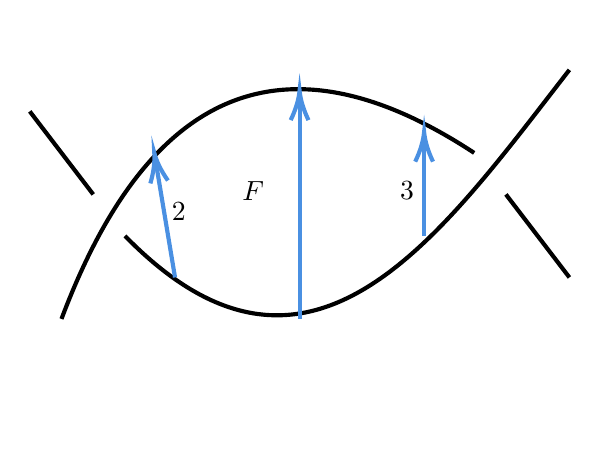
\begin{tikzpicture}[x=0.75pt,y=0.75pt,yscale=-1,xscale=1]
%uncomment if require: \path (0,877); %set diagram left start at 0, and has height of 877

%Curve Lines [id:da19609189587014564] 
\draw [line width=1.5]    (195.29,140) .. controls (237.61,27.33) and (303.88,0.67) .. (394.12,60) ;
%Straight Lines [id:da2771116463618114] 
\draw [line width=1.5]    (180,40) -- (210.59,80) ;
%Curve Lines [id:da5075059974941536] 
\draw [line width=1.5]    (225.88,100) .. controls (315.1,191.33) and (377.29,100.67) .. (440,20) ;
%Straight Lines [id:da01404980269438516] 
\draw [line width=1.5]    (409.41,80) -- (440,120) ;
%Straight Lines [id:da6027225475778994] 
\draw [color={rgb, 255:red, 74; green, 144; blue, 226 }  ,draw opacity=1 ][line width=1.5]    (250,120) -- (240.49,62.96) ;
\draw [shift={(240,60)}, rotate = 80.54] [color={rgb, 255:red, 74; green, 144; blue, 226 }  ,draw opacity=1 ][line width=1.5]    (14.21,-4.28) .. controls (9.04,-1.82) and (4.3,-0.39) .. (0,0) .. controls (4.3,0.39) and (9.04,1.82) .. (14.21,4.28)   ;
%Straight Lines [id:da602091940582576] 
\draw [color={rgb, 255:red, 74; green, 144; blue, 226 }  ,draw opacity=1 ][line width=1.5]    (370,100) -- (370,53) ;
\draw [shift={(370,50)}, rotate = 90] [color={rgb, 255:red, 74; green, 144; blue, 226 }  ,draw opacity=1 ][line width=1.5]    (14.21,-4.28) .. controls (9.04,-1.82) and (4.3,-0.39) .. (0,0) .. controls (4.3,0.39) and (9.04,1.82) .. (14.21,4.28)   ;
%Straight Lines [id:da7589682295521507] 
\draw [color={rgb, 255:red, 74; green, 144; blue, 226 }  ,draw opacity=1 ][line width=1.5]    (310,140) -- (310,33) ;
\draw [shift={(310,30)}, rotate = 90] [color={rgb, 255:red, 74; green, 144; blue, 226 }  ,draw opacity=1 ][line width=1.5]    (14.21,-4.28) .. controls (9.04,-1.82) and (4.3,-0.39) .. (0,0) .. controls (4.3,0.39) and (9.04,1.82) .. (14.21,4.28)   ;

% Text Node
\draw (281,72.4) node [anchor=north west][inner sep=0.75pt]    {$F$};
% Text Node
\draw (247,82.4) node [anchor=north west][inner sep=0.75pt]    {$2$};
% Text Node
\draw (357,72.4) node [anchor=north west][inner sep=0.75pt]    {$3$};


\end{tikzpicture}
        \caption{Isotopia de la Region F}
    \end{figure}
    En general en regiones así siempre las aristas entre cruces serán isotopicas, luego basta con tener una para tener toda la información, por lo que estas regiones pueden colapsarse en los diagramas finales a solo una arista y eliminar la cara completamente obteniendo la presentación dada por Thurston original, dos tetraedros, en este caso aplanados y uno visto desde adentro, donde la arista 0 se identifica con la 1 y la arista 2 con la 3, note ademas que cambiamos la numeración por lineas en las aristas, esto sera útil luego para no sobrecargar el dibujo.
    \begin{figure}[H]
    \centering
    \input{tetra8}
       \caption{Tetraedros del nudo de 8 luego de contraer las regiones E y F.} 
    \end{figure}
\end{note}
\subsection{Otros ejemplos de descompocision y una vista a la generalización}
El proceso realizado antes funciona muy bien tanto para enlaces como para nudos, para mostrar esto haremos uno de cada uno
\begin{eg}
    Considere la proyección del enlace de Whitehead estándar con regiones y aristas ya identificadas
    \begin{figure}[H]
    \centering
    
%!TEX root = ./main.tex

\tikzset{every picture/.style={line width=0.75pt}} %set default line width to 0.75pt        

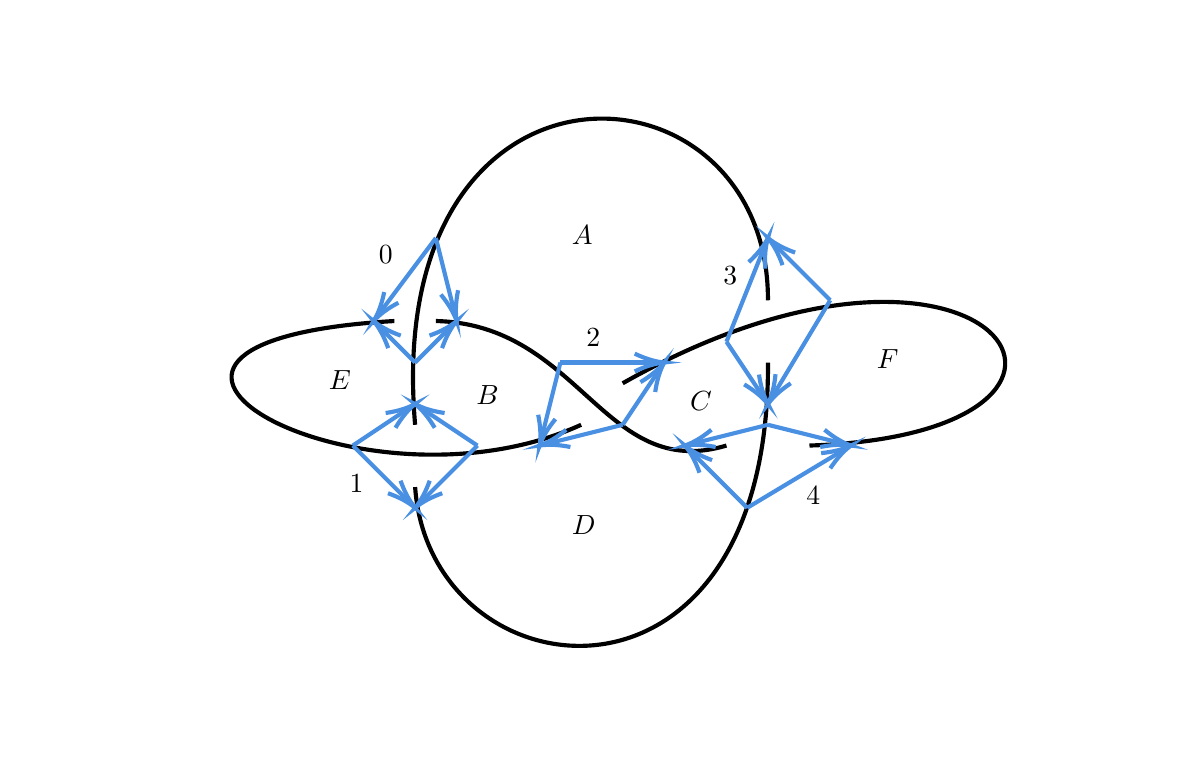
\begin{tikzpicture}[x=0.75pt,y=0.75pt,yscale=-1,xscale=1]
%uncomment if require: \path (0,877); %set diagram left start at 0, and has height of 877

%Curve Lines [id:da1815470268489796] 
\draw [line width=1.5]    (190,150) .. controls (173.67,-40.33) and (360.33,-31) .. (360,90) ;
%Curve Lines [id:da1886044146181638] 
\draw [line width=1.5]    (190,180) .. controls (197,281) and (361,301.67) .. (360,120) ;
%Curve Lines [id:da5499420166410015] 
\draw [line width=1.5]    (270,150) .. controls (163.67,198.33) and (4.33,110.33) .. (180,100) ;
%Curve Lines [id:da628102200884786] 
\draw [line width=1.5]    (290,130) .. controls (468.33,29) and (552.33,154.33) .. (380,160) ;
%Curve Lines [id:da6746806126730861] 
\draw [line width=1.5]    (200,100) .. controls (269.67,101.67) and (281,177.67) .. (340,160) ;
%Straight Lines [id:da6086058360131362] 
\draw [color={rgb, 255:red, 74; green, 144; blue, 226 }  ,draw opacity=1 ][line width=1.5]    (200,60) -- (209.27,97.09) ;
\draw [shift={(210,100)}, rotate = 255.96] [color={rgb, 255:red, 74; green, 144; blue, 226 }  ,draw opacity=1 ][line width=1.5]    (14.21,-4.28) .. controls (9.04,-1.82) and (4.3,-0.39) .. (0,0) .. controls (4.3,0.39) and (9.04,1.82) .. (14.21,4.28)   ;
%Straight Lines [id:da014067308052953753] 
\draw [color={rgb, 255:red, 74; green, 144; blue, 226 }  ,draw opacity=1 ][line width=1.5]    (200,60) -- (171.8,97.6) ;
\draw [shift={(170,100)}, rotate = 306.87] [color={rgb, 255:red, 74; green, 144; blue, 226 }  ,draw opacity=1 ][line width=1.5]    (14.21,-4.28) .. controls (9.04,-1.82) and (4.3,-0.39) .. (0,0) .. controls (4.3,0.39) and (9.04,1.82) .. (14.21,4.28)   ;
%Straight Lines [id:da6519101916534229] 
\draw [color={rgb, 255:red, 74; green, 144; blue, 226 }  ,draw opacity=1 ][line width=1.5]    (190,120) -- (172.12,102.12) ;
\draw [shift={(170,100)}, rotate = 45] [color={rgb, 255:red, 74; green, 144; blue, 226 }  ,draw opacity=1 ][line width=1.5]    (14.21,-4.28) .. controls (9.04,-1.82) and (4.3,-0.39) .. (0,0) .. controls (4.3,0.39) and (9.04,1.82) .. (14.21,4.28)   ;
%Straight Lines [id:da8188548073525511] 
\draw [color={rgb, 255:red, 74; green, 144; blue, 226 }  ,draw opacity=1 ][line width=1.5]    (190,120) -- (207.88,102.12) ;
\draw [shift={(210,100)}, rotate = 135] [color={rgb, 255:red, 74; green, 144; blue, 226 }  ,draw opacity=1 ][line width=1.5]    (14.21,-4.28) .. controls (9.04,-1.82) and (4.3,-0.39) .. (0,0) .. controls (4.3,0.39) and (9.04,1.82) .. (14.21,4.28)   ;
%Straight Lines [id:da9049936130099601] 
\draw [color={rgb, 255:red, 74; green, 144; blue, 226 }  ,draw opacity=1 ][line width=1.5]    (220,160) -- (192.5,141.66) ;
\draw [shift={(190,140)}, rotate = 33.69] [color={rgb, 255:red, 74; green, 144; blue, 226 }  ,draw opacity=1 ][line width=1.5]    (14.21,-4.28) .. controls (9.04,-1.82) and (4.3,-0.39) .. (0,0) .. controls (4.3,0.39) and (9.04,1.82) .. (14.21,4.28)   ;
%Straight Lines [id:da0032696330086658953] 
\draw [color={rgb, 255:red, 74; green, 144; blue, 226 }  ,draw opacity=1 ][line width=1.5]    (220,160) -- (192.12,187.88) ;
\draw [shift={(190,190)}, rotate = 315] [color={rgb, 255:red, 74; green, 144; blue, 226 }  ,draw opacity=1 ][line width=1.5]    (14.21,-4.28) .. controls (9.04,-1.82) and (4.3,-0.39) .. (0,0) .. controls (4.3,0.39) and (9.04,1.82) .. (14.21,4.28)   ;
%Straight Lines [id:da6624458862731804] 
\draw [color={rgb, 255:red, 74; green, 144; blue, 226 }  ,draw opacity=1 ][line width=1.5]    (160,160) -- (187.88,187.88) ;
\draw [shift={(190,190)}, rotate = 225] [color={rgb, 255:red, 74; green, 144; blue, 226 }  ,draw opacity=1 ][line width=1.5]    (14.21,-4.28) .. controls (9.04,-1.82) and (4.3,-0.39) .. (0,0) .. controls (4.3,0.39) and (9.04,1.82) .. (14.21,4.28)   ;
%Straight Lines [id:da9943610350622754] 
\draw [color={rgb, 255:red, 74; green, 144; blue, 226 }  ,draw opacity=1 ][line width=1.5]    (160,160) -- (187.5,141.66) ;
\draw [shift={(190,140)}, rotate = 146.31] [color={rgb, 255:red, 74; green, 144; blue, 226 }  ,draw opacity=1 ][line width=1.5]    (14.21,-4.28) .. controls (9.04,-1.82) and (4.3,-0.39) .. (0,0) .. controls (4.3,0.39) and (9.04,1.82) .. (14.21,4.28)   ;
%Straight Lines [id:da7835353652276644] 
\draw [color={rgb, 255:red, 74; green, 144; blue, 226 }  ,draw opacity=1 ][line width=1.5]    (260,120) -- (250.73,157.09) ;
\draw [shift={(250,160)}, rotate = 284.04] [color={rgb, 255:red, 74; green, 144; blue, 226 }  ,draw opacity=1 ][line width=1.5]    (14.21,-4.28) .. controls (9.04,-1.82) and (4.3,-0.39) .. (0,0) .. controls (4.3,0.39) and (9.04,1.82) .. (14.21,4.28)   ;
%Straight Lines [id:da45301259693483675] 
\draw [color={rgb, 255:red, 74; green, 144; blue, 226 }  ,draw opacity=1 ][line width=1.5]    (290,150) -- (252.91,159.27) ;
\draw [shift={(250,160)}, rotate = 345.96] [color={rgb, 255:red, 74; green, 144; blue, 226 }  ,draw opacity=1 ][line width=1.5]    (14.21,-4.28) .. controls (9.04,-1.82) and (4.3,-0.39) .. (0,0) .. controls (4.3,0.39) and (9.04,1.82) .. (14.21,4.28)   ;
%Straight Lines [id:da4594824971051823] 
\draw [color={rgb, 255:red, 74; green, 144; blue, 226 }  ,draw opacity=1 ][line width=1.5]    (260,120) -- (307,120) ;
\draw [shift={(310,120)}, rotate = 180] [color={rgb, 255:red, 74; green, 144; blue, 226 }  ,draw opacity=1 ][line width=1.5]    (14.21,-4.28) .. controls (9.04,-1.82) and (4.3,-0.39) .. (0,0) .. controls (4.3,0.39) and (9.04,1.82) .. (14.21,4.28)   ;
%Straight Lines [id:da1631157459977307] 
\draw [color={rgb, 255:red, 74; green, 144; blue, 226 }  ,draw opacity=1 ][line width=1.5]    (290,150) -- (308.34,122.5) ;
\draw [shift={(310,120)}, rotate = 123.69] [color={rgb, 255:red, 74; green, 144; blue, 226 }  ,draw opacity=1 ][line width=1.5]    (14.21,-4.28) .. controls (9.04,-1.82) and (4.3,-0.39) .. (0,0) .. controls (4.3,0.39) and (9.04,1.82) .. (14.21,4.28)   ;
%Straight Lines [id:da8901598603000586] 
\draw [color={rgb, 255:red, 74; green, 144; blue, 226 }  ,draw opacity=1 ][line width=1.5]    (340,110) -- (358.34,137.5) ;
\draw [shift={(360,140)}, rotate = 236.31] [color={rgb, 255:red, 74; green, 144; blue, 226 }  ,draw opacity=1 ][line width=1.5]    (14.21,-4.28) .. controls (9.04,-1.82) and (4.3,-0.39) .. (0,0) .. controls (4.3,0.39) and (9.04,1.82) .. (14.21,4.28)   ;
%Straight Lines [id:da28864384570380464] 
\draw [color={rgb, 255:red, 74; green, 144; blue, 226 }  ,draw opacity=1 ][line width=1.5]    (390,90) -- (361.54,137.43) ;
\draw [shift={(360,140)}, rotate = 300.96] [color={rgb, 255:red, 74; green, 144; blue, 226 }  ,draw opacity=1 ][line width=1.5]    (14.21,-4.28) .. controls (9.04,-1.82) and (4.3,-0.39) .. (0,0) .. controls (4.3,0.39) and (9.04,1.82) .. (14.21,4.28)   ;
%Straight Lines [id:da7479932996118415] 
\draw [color={rgb, 255:red, 74; green, 144; blue, 226 }  ,draw opacity=1 ][line width=1.5]    (340,110) -- (358.89,62.79) ;
\draw [shift={(360,60)}, rotate = 111.8] [color={rgb, 255:red, 74; green, 144; blue, 226 }  ,draw opacity=1 ][line width=1.5]    (14.21,-4.28) .. controls (9.04,-1.82) and (4.3,-0.39) .. (0,0) .. controls (4.3,0.39) and (9.04,1.82) .. (14.21,4.28)   ;
%Straight Lines [id:da21649314531412311] 
\draw [color={rgb, 255:red, 74; green, 144; blue, 226 }  ,draw opacity=1 ][line width=1.5]    (390,90) -- (362.12,62.12) ;
\draw [shift={(360,60)}, rotate = 45] [color={rgb, 255:red, 74; green, 144; blue, 226 }  ,draw opacity=1 ][line width=1.5]    (14.21,-4.28) .. controls (9.04,-1.82) and (4.3,-0.39) .. (0,0) .. controls (4.3,0.39) and (9.04,1.82) .. (14.21,4.28)   ;
%Straight Lines [id:da07141714735873272] 
\draw [color={rgb, 255:red, 74; green, 144; blue, 226 }  ,draw opacity=1 ][line width=1.5]    (350,190) -- (322.12,162.12) ;
\draw [shift={(320,160)}, rotate = 45] [color={rgb, 255:red, 74; green, 144; blue, 226 }  ,draw opacity=1 ][line width=1.5]    (14.21,-4.28) .. controls (9.04,-1.82) and (4.3,-0.39) .. (0,0) .. controls (4.3,0.39) and (9.04,1.82) .. (14.21,4.28)   ;
%Straight Lines [id:da761624160799076] 
\draw [color={rgb, 255:red, 74; green, 144; blue, 226 }  ,draw opacity=1 ][line width=1.5]    (360,150) -- (322.91,159.27) ;
\draw [shift={(320,160)}, rotate = 345.96] [color={rgb, 255:red, 74; green, 144; blue, 226 }  ,draw opacity=1 ][line width=1.5]    (14.21,-4.28) .. controls (9.04,-1.82) and (4.3,-0.39) .. (0,0) .. controls (4.3,0.39) and (9.04,1.82) .. (14.21,4.28)   ;
%Straight Lines [id:da8783890100064231] 
\draw [color={rgb, 255:red, 74; green, 144; blue, 226 }  ,draw opacity=1 ][line width=1.5]    (350,190) -- (397.43,161.54) ;
\draw [shift={(400,160)}, rotate = 149.04] [color={rgb, 255:red, 74; green, 144; blue, 226 }  ,draw opacity=1 ][line width=1.5]    (14.21,-4.28) .. controls (9.04,-1.82) and (4.3,-0.39) .. (0,0) .. controls (4.3,0.39) and (9.04,1.82) .. (14.21,4.28)   ;
%Straight Lines [id:da8165383548278232] 
\draw [color={rgb, 255:red, 74; green, 144; blue, 226 }  ,draw opacity=1 ][line width=1.5]    (360,150) -- (397.09,159.27) ;
\draw [shift={(400,160)}, rotate = 194.04] [color={rgb, 255:red, 74; green, 144; blue, 226 }  ,draw opacity=1 ][line width=1.5]    (14.21,-4.28) .. controls (9.04,-1.82) and (4.3,-0.39) .. (0,0) .. controls (4.3,0.39) and (9.04,1.82) .. (14.21,4.28)   ;

% Text Node
\draw (264,52.4) node [anchor=north west][inner sep=0.75pt]    {$A$};
% Text Node
\draw (218,129.4) node [anchor=north west][inner sep=0.75pt]    {$B$};
% Text Node
\draw (321,132.4) node [anchor=north west][inner sep=0.75pt]    {$C$};
% Text Node
\draw (264,192.4) node [anchor=north west][inner sep=0.75pt]    {$D$};
% Text Node
\draw (147,122.4) node [anchor=north west][inner sep=0.75pt]    {$E$};
% Text Node
\draw (411,112.4) node [anchor=north west][inner sep=0.75pt]    {$F$};
% Text Node
\draw (171,62.4) node [anchor=north west][inner sep=0.75pt]    {$0$};
% Text Node
\draw (157,172.4) node [anchor=north west][inner sep=0.75pt]    {$1$};
% Text Node
\draw (271,102.4) node [anchor=north west][inner sep=0.75pt]    {$2$};
% Text Node
\draw (337,72.4) node [anchor=north west][inner sep=0.75pt]    {$3$};
% Text Node
\draw (377,178.4) node [anchor=north west][inner sep=0.75pt]    {$4$};


\end{tikzpicture}
        \caption{enlace de Whitehead}
    \end{figure}
    Siguiendo los pasos indicados antes obtenemos los siguientes diagramas que nos dan ambos poliedros, el de arriba visto desde adentro y el de abajo visto desde afuera.
    \begin{figure}[H]
    \centering
    %!TEX root = ./main.tex



\tikzset{every picture/.style={line width=0.75pt}} %set default line width to 0.75pt        

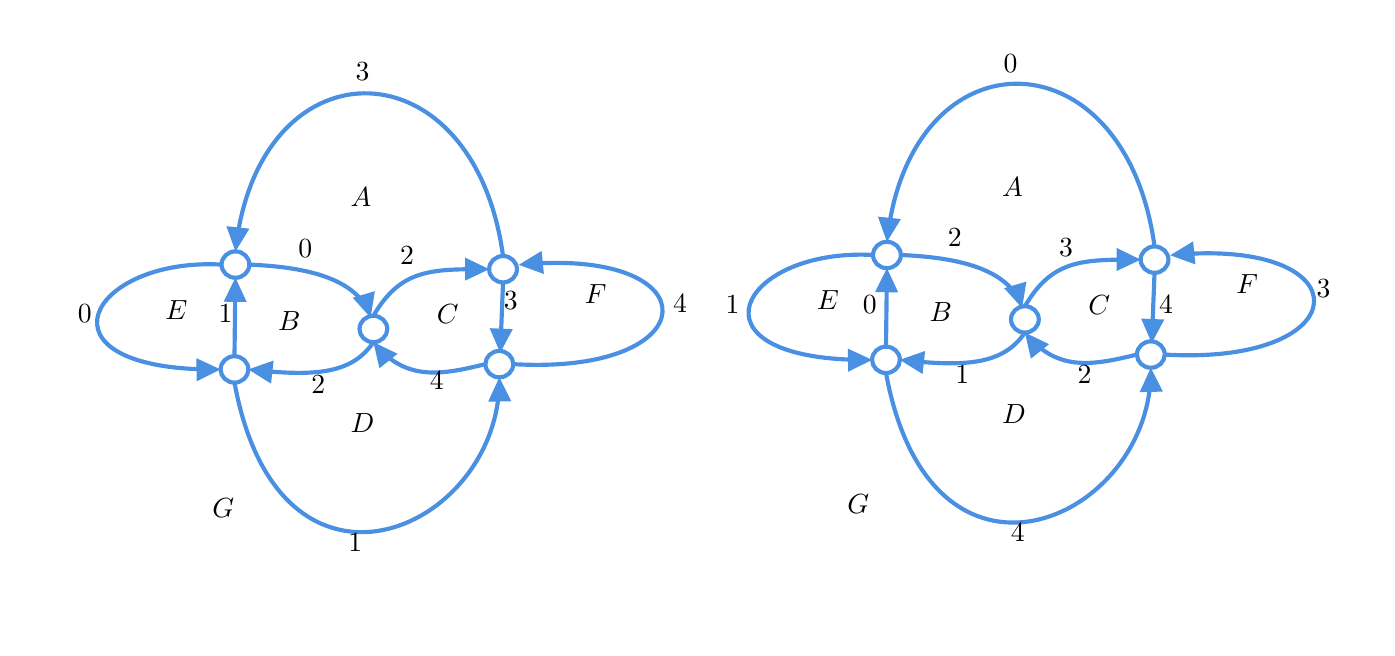
\begin{tikzpicture}[x=0.75pt,y=0.75pt,yscale=-1,xscale=1]
%uncomment if require: \path (0,877); %set diagram left start at 0, and has height of 877

%Straight Lines [id:da9943610350622754] 
\draw [color={rgb, 255:red, 74; green, 144; blue, 226 }  ,draw opacity=1 ][line width=1.5]    (97.18,155.15) -- (97.59,121.34) ;
\draw [shift={(97.64,117.34)}, rotate = 90.69] [fill={rgb, 255:red, 74; green, 144; blue, 226 }  ,fill opacity=1 ][line width=0.08]  [draw opacity=0] (11.61,-5.58) -- (0,0) -- (11.61,5.58) -- cycle    ;
%Straight Lines [id:da28864384570380464] 
\draw [color={rgb, 255:red, 74; green, 144; blue, 226 }  ,draw opacity=1 ][line width=1.5]    (226.57,119.58) -- (225.39,149.46) ;
\draw [shift={(225.23,153.46)}, rotate = 272.26] [fill={rgb, 255:red, 74; green, 144; blue, 226 }  ,fill opacity=1 ][line width=0.08]  [draw opacity=0] (11.61,-5.58) -- (0,0) -- (11.61,5.58) -- cycle    ;
%Shape: Ellipse [id:dp029827328935257524] 
\draw  [color={rgb, 255:red, 74; green, 144; blue, 226 }  ,draw opacity=1 ][fill={rgb, 255:red, 255; green, 255; blue, 255 }  ,fill opacity=1 ][line width=1.5]  (90.95,110.99) .. controls (90.95,107.48) and (93.95,104.64) .. (97.64,104.64) .. controls (101.34,104.64) and (104.33,107.48) .. (104.33,110.99) .. controls (104.33,114.5) and (101.34,117.34) .. (97.64,117.34) .. controls (93.95,117.34) and (90.95,114.5) .. (90.95,110.99) -- cycle ;
%Shape: Ellipse [id:dp4202696786928657] 
\draw  [color={rgb, 255:red, 74; green, 144; blue, 226 }  ,draw opacity=1 ][fill={rgb, 255:red, 255; green, 255; blue, 255 }  ,fill opacity=1 ][line width=1.5]  (90.49,161.51) .. controls (90.49,158) and (93.49,155.15) .. (97.18,155.15) .. controls (100.88,155.15) and (103.88,158) .. (103.88,161.51) .. controls (103.88,165.01) and (100.88,167.86) .. (97.18,167.86) .. controls (93.49,167.86) and (90.49,165.01) .. (90.49,161.51) -- cycle ;
%Shape: Ellipse [id:dp7878916678981432] 
\draw  [color={rgb, 255:red, 74; green, 144; blue, 226 }  ,draw opacity=1 ][fill={rgb, 255:red, 255; green, 255; blue, 255 }  ,fill opacity=1 ][line width=1.5]  (157.42,142.03) .. controls (157.42,138.52) and (160.41,135.67) .. (164.11,135.67) .. controls (167.8,135.67) and (170.8,138.52) .. (170.8,142.03) .. controls (170.8,145.53) and (167.8,148.38) .. (164.11,148.38) .. controls (160.41,148.38) and (157.42,145.53) .. (157.42,142.03) -- cycle ;
%Shape: Ellipse [id:dp9437208822572988] 
\draw  [color={rgb, 255:red, 74; green, 144; blue, 226 }  ,draw opacity=1 ][fill={rgb, 255:red, 255; green, 255; blue, 255 }  ,fill opacity=1 ][line width=1.5]  (219.88,113.23) .. controls (219.88,109.72) and (222.87,106.88) .. (226.57,106.88) .. controls (230.27,106.88) and (233.26,109.72) .. (233.26,113.23) .. controls (233.26,116.74) and (230.27,119.58) .. (226.57,119.58) .. controls (222.87,119.58) and (219.88,116.74) .. (219.88,113.23) -- cycle ;
%Shape: Ellipse [id:dp06226933559817249] 
\draw  [color={rgb, 255:red, 74; green, 144; blue, 226 }  ,draw opacity=1 ][fill={rgb, 255:red, 255; green, 255; blue, 255 }  ,fill opacity=1 ][line width=1.5]  (218.09,158.96) .. controls (218.09,155.46) and (221.09,152.61) .. (224.78,152.61) .. controls (228.48,152.61) and (231.48,155.46) .. (231.48,158.96) .. controls (231.48,162.47) and (228.48,165.32) .. (224.78,165.32) .. controls (221.09,165.32) and (218.09,162.47) .. (218.09,158.96) -- cycle ;
%Curve Lines [id:da2979171995828367] 
\draw [color={rgb, 255:red, 74; green, 144; blue, 226 }  ,draw opacity=1 ][line width=1.5]    (98.19,100.11) .. controls (111.44,2.47) and (212.65,4.55) .. (226.57,106.88) ;
\draw [shift={(97.64,104.64)}, rotate = 275.97] [fill={rgb, 255:red, 74; green, 144; blue, 226 }  ,fill opacity=1 ][line width=0.08]  [draw opacity=0] (11.61,-5.58) -- (0,0) -- (11.61,5.58) -- cycle    ;
%Curve Lines [id:da8764254520788726] 
\draw [color={rgb, 255:red, 74; green, 144; blue, 226 }  ,draw opacity=1 ][line width=1.5]    (104.33,110.99) .. controls (124.31,111.9) and (152.85,115.08) .. (161.39,132.92) ;
\draw [shift={(162.77,136.52)}, rotate = 253.46] [fill={rgb, 255:red, 74; green, 144; blue, 226 }  ,fill opacity=1 ][line width=0.08]  [draw opacity=0] (11.61,-5.58) -- (0,0) -- (11.61,5.58) -- cycle    ;
%Curve Lines [id:da809160987469365] 
\draw [color={rgb, 255:red, 74; green, 144; blue, 226 }  ,draw opacity=1 ][line width=1.5]    (86.4,161.52) .. controls (-1.46,161.13) and (26.63,107.5) .. (90.95,110.99) ;
\draw [shift={(90.49,161.51)}, rotate = 179.22] [fill={rgb, 255:red, 74; green, 144; blue, 226 }  ,fill opacity=1 ][line width=0.08]  [draw opacity=0] (11.61,-5.58) -- (0,0) -- (11.61,5.58) -- cycle    ;
%Curve Lines [id:da9659495047647262] 
\draw [color={rgb, 255:red, 74; green, 144; blue, 226 }  ,draw opacity=1 ][line width=1.5]    (97.18,167.86) .. controls (118.72,285.2) and (222.93,239.85) .. (224.77,168.59) ;
\draw [shift={(224.78,165.32)}, rotate = 88.95] [fill={rgb, 255:red, 74; green, 144; blue, 226 }  ,fill opacity=1 ][line width=0.08]  [draw opacity=0] (11.61,-5.58) -- (0,0) -- (11.61,5.58) -- cycle    ;
%Curve Lines [id:da5397459745235432] 
\draw [color={rgb, 255:red, 74; green, 144; blue, 226 }  ,draw opacity=1 ][line width=1.5]    (164.11,148.38) .. controls (153.97,163.28) and (137.12,164.92) .. (107.63,161.91) ;
\draw [shift={(103.88,161.51)}, rotate = 6.33] [fill={rgb, 255:red, 74; green, 144; blue, 226 }  ,fill opacity=1 ][line width=0.08]  [draw opacity=0] (11.61,-5.58) -- (0,0) -- (11.61,5.58) -- cycle    ;
%Curve Lines [id:da4211882280413548] 
\draw [color={rgb, 255:red, 74; green, 144; blue, 226 }  ,draw opacity=1 ][line width=1.5]    (164.11,135.67) .. controls (176.75,114.11) and (190.34,113.14) .. (216.15,113.22) ;
\draw [shift={(219.88,113.23)}, rotate = 180.29] [fill={rgb, 255:red, 74; green, 144; blue, 226 }  ,fill opacity=1 ][line width=0.08]  [draw opacity=0] (11.61,-5.58) -- (0,0) -- (11.61,5.58) -- cycle    ;
%Curve Lines [id:da956839943660936] 
\draw [color={rgb, 255:red, 74; green, 144; blue, 226 }  ,draw opacity=1 ][line width=1.5]    (218.09,158.96) .. controls (198.7,163.63) and (181.69,167.42) .. (166.7,151.38) ;
\draw [shift={(164.11,148.38)}, rotate = 51.28] [fill={rgb, 255:red, 74; green, 144; blue, 226 }  ,fill opacity=1 ][line width=0.08]  [draw opacity=0] (11.61,-5.58) -- (0,0) -- (11.61,5.58) -- cycle    ;
%Curve Lines [id:da8737526251165968] 
\draw [color={rgb, 255:red, 74; green, 144; blue, 226 }  ,draw opacity=1 ][line width=1.5]    (231.48,158.96) .. controls (325.12,164.41) and (327.8,103.05) .. (236.94,110.86) ;
\draw [shift={(234.15,111.11)}, rotate = 354.32] [fill={rgb, 255:red, 74; green, 144; blue, 226 }  ,fill opacity=1 ][line width=0.08]  [draw opacity=0] (11.61,-5.58) -- (0,0) -- (11.61,5.58) -- cycle    ;
%Straight Lines [id:da7109511854568149] 
\draw [color={rgb, 255:red, 74; green, 144; blue, 226 }  ,draw opacity=1 ][line width=1.5]    (411.08,150.53) -- (411.49,116.72) ;
\draw [shift={(411.53,112.72)}, rotate = 90.69] [fill={rgb, 255:red, 74; green, 144; blue, 226 }  ,fill opacity=1 ][line width=0.08]  [draw opacity=0] (11.61,-5.58) -- (0,0) -- (11.61,5.58) -- cycle    ;
%Straight Lines [id:da49493506455500713] 
\draw [color={rgb, 255:red, 74; green, 144; blue, 226 }  ,draw opacity=1 ][line width=1.5]    (540.46,114.96) -- (539.28,144.84) ;
\draw [shift={(539.12,148.84)}, rotate = 272.26] [fill={rgb, 255:red, 74; green, 144; blue, 226 }  ,fill opacity=1 ][line width=0.08]  [draw opacity=0] (11.61,-5.58) -- (0,0) -- (11.61,5.58) -- cycle    ;
%Shape: Ellipse [id:dp9403539709464994] 
\draw  [color={rgb, 255:red, 74; green, 144; blue, 226 }  ,draw opacity=1 ][fill={rgb, 255:red, 255; green, 255; blue, 255 }  ,fill opacity=1 ][line width=1.5]  (404.84,106.37) .. controls (404.84,102.86) and (407.84,100.02) .. (411.53,100.02) .. controls (415.23,100.02) and (418.23,102.86) .. (418.23,106.37) .. controls (418.23,109.88) and (415.23,112.72) .. (411.53,112.72) .. controls (407.84,112.72) and (404.84,109.88) .. (404.84,106.37) -- cycle ;
%Shape: Ellipse [id:dp9543762925369562] 
\draw  [color={rgb, 255:red, 74; green, 144; blue, 226 }  ,draw opacity=1 ][fill={rgb, 255:red, 255; green, 255; blue, 255 }  ,fill opacity=1 ][line width=1.5]  (404.38,156.89) .. controls (404.38,153.38) and (407.38,150.53) .. (411.08,150.53) .. controls (414.77,150.53) and (417.77,153.38) .. (417.77,156.89) .. controls (417.77,160.39) and (414.77,163.24) .. (411.08,163.24) .. controls (407.38,163.24) and (404.38,160.39) .. (404.38,156.89) -- cycle ;
%Shape: Ellipse [id:dp6094250043745837] 
\draw  [color={rgb, 255:red, 74; green, 144; blue, 226 }  ,draw opacity=1 ][fill={rgb, 255:red, 255; green, 255; blue, 255 }  ,fill opacity=1 ][line width=1.5]  (471.31,137.41) .. controls (471.31,133.9) and (474.3,131.06) .. (478,131.06) .. controls (481.7,131.06) and (484.69,133.9) .. (484.69,137.41) .. controls (484.69,140.92) and (481.7,143.76) .. (478,143.76) .. controls (474.3,143.76) and (471.31,140.92) .. (471.31,137.41) -- cycle ;
%Shape: Ellipse [id:dp7048265837255207] 
\draw  [color={rgb, 255:red, 74; green, 144; blue, 226 }  ,draw opacity=1 ][fill={rgb, 255:red, 255; green, 255; blue, 255 }  ,fill opacity=1 ][line width=1.5]  (533.77,108.61) .. controls (533.77,105.1) and (536.77,102.26) .. (540.46,102.26) .. controls (544.16,102.26) and (547.15,105.1) .. (547.15,108.61) .. controls (547.15,112.12) and (544.16,114.96) .. (540.46,114.96) .. controls (536.77,114.96) and (533.77,112.12) .. (533.77,108.61) -- cycle ;
%Shape: Ellipse [id:dp8750927184704229] 
\draw  [color={rgb, 255:red, 74; green, 144; blue, 226 }  ,draw opacity=1 ][fill={rgb, 255:red, 255; green, 255; blue, 255 }  ,fill opacity=1 ][line width=1.5]  (531.98,154.35) .. controls (531.98,150.84) and (534.98,147.99) .. (538.68,147.99) .. controls (542.37,147.99) and (545.37,150.84) .. (545.37,154.35) .. controls (545.37,157.85) and (542.37,160.7) .. (538.68,160.7) .. controls (534.98,160.7) and (531.98,157.85) .. (531.98,154.35) -- cycle ;
%Curve Lines [id:da5236484284848602] 
\draw [color={rgb, 255:red, 74; green, 144; blue, 226 }  ,draw opacity=1 ][line width=1.5]    (412.08,95.49) .. controls (425.33,-2.15) and (526.55,-0.07) .. (540.46,102.26) ;
\draw [shift={(411.53,100.02)}, rotate = 275.97] [fill={rgb, 255:red, 74; green, 144; blue, 226 }  ,fill opacity=1 ][line width=0.08]  [draw opacity=0] (11.61,-5.58) -- (0,0) -- (11.61,5.58) -- cycle    ;
%Curve Lines [id:da9662673859391505] 
\draw [color={rgb, 255:red, 74; green, 144; blue, 226 }  ,draw opacity=1 ][line width=1.5]    (418.23,106.37) .. controls (438.21,107.28) and (466.74,110.46) .. (475.28,128.3) ;
\draw [shift={(476.66,131.9)}, rotate = 253.46] [fill={rgb, 255:red, 74; green, 144; blue, 226 }  ,fill opacity=1 ][line width=0.08]  [draw opacity=0] (11.61,-5.58) -- (0,0) -- (11.61,5.58) -- cycle    ;
%Curve Lines [id:da2629698729180272] 
\draw [color={rgb, 255:red, 74; green, 144; blue, 226 }  ,draw opacity=1 ][line width=1.5]    (400.29,156.91) .. controls (312.43,156.51) and (340.52,102.88) .. (404.84,106.37) ;
\draw [shift={(404.38,156.89)}, rotate = 179.22] [fill={rgb, 255:red, 74; green, 144; blue, 226 }  ,fill opacity=1 ][line width=0.08]  [draw opacity=0] (11.61,-5.58) -- (0,0) -- (11.61,5.58) -- cycle    ;
%Curve Lines [id:da48834267482785687] 
\draw [color={rgb, 255:red, 74; green, 144; blue, 226 }  ,draw opacity=1 ][line width=1.5]    (411.08,163.24) .. controls (432.61,280.58) and (536.82,235.23) .. (538.66,163.97) ;
\draw [shift={(538.68,160.7)}, rotate = 88.95] [fill={rgb, 255:red, 74; green, 144; blue, 226 }  ,fill opacity=1 ][line width=0.08]  [draw opacity=0] (11.61,-5.58) -- (0,0) -- (11.61,5.58) -- cycle    ;
%Curve Lines [id:da8150566103908512] 
\draw [color={rgb, 255:red, 74; green, 144; blue, 226 }  ,draw opacity=1 ][line width=1.5]    (478,143.76) .. controls (467.86,158.66) and (451.01,160.3) .. (421.52,157.29) ;
\draw [shift={(417.77,156.89)}, rotate = 6.33] [fill={rgb, 255:red, 74; green, 144; blue, 226 }  ,fill opacity=1 ][line width=0.08]  [draw opacity=0] (11.61,-5.58) -- (0,0) -- (11.61,5.58) -- cycle    ;
%Curve Lines [id:da4757930219164036] 
\draw [color={rgb, 255:red, 74; green, 144; blue, 226 }  ,draw opacity=1 ][line width=1.5]    (478,131.06) .. controls (490.64,109.49) and (504.23,108.52) .. (530.04,108.6) ;
\draw [shift={(533.77,108.61)}, rotate = 180.29] [fill={rgb, 255:red, 74; green, 144; blue, 226 }  ,fill opacity=1 ][line width=0.08]  [draw opacity=0] (11.61,-5.58) -- (0,0) -- (11.61,5.58) -- cycle    ;
%Curve Lines [id:da9886701870479793] 
\draw [color={rgb, 255:red, 74; green, 144; blue, 226 }  ,draw opacity=1 ][line width=1.5]    (531.98,154.35) .. controls (512.59,159.01) and (495.59,162.8) .. (480.6,146.76) ;
\draw [shift={(478,143.76)}, rotate = 51.28] [fill={rgb, 255:red, 74; green, 144; blue, 226 }  ,fill opacity=1 ][line width=0.08]  [draw opacity=0] (11.61,-5.58) -- (0,0) -- (11.61,5.58) -- cycle    ;
%Curve Lines [id:da21521285354906916] 
\draw [color={rgb, 255:red, 74; green, 144; blue, 226 }  ,draw opacity=1 ][line width=1.5]    (545.37,154.35) .. controls (639.01,159.8) and (641.69,98.43) .. (550.83,106.24) ;
\draw [shift={(548.05,106.5)}, rotate = 354.32] [fill={rgb, 255:red, 74; green, 144; blue, 226 }  ,fill opacity=1 ][line width=0.08]  [draw opacity=0] (11.61,-5.58) -- (0,0) -- (11.61,5.58) -- cycle    ;

% Text Node
\draw (151.61,72.18) node [anchor=north west][inner sep=0.75pt]    {$A$};
% Text Node
\draw (116.72,132.26) node [anchor=north west][inner sep=0.75pt]    {$B$};
% Text Node
\draw (193.25,128.92) node [anchor=north west][inner sep=0.75pt]    {$C$};
% Text Node
\draw (151.61,181.41) node [anchor=north west][inner sep=0.75pt]    {$D$};
% Text Node
\draw (62.33,126.8) node [anchor=north west][inner sep=0.75pt]    {$E$};
% Text Node
\draw (264.56,118.99) node [anchor=north west][inner sep=0.75pt]    {$F$};
% Text Node
\draw (20.25,128.92) node [anchor=north west][inner sep=0.75pt]    {$0$};
% Text Node
\draw (150.52,239.02) node [anchor=north west][inner sep=0.75pt]    {$1$};
% Text Node
\draw (175.51,100.97) node [anchor=north west][inner sep=0.75pt]    {$2$};
% Text Node
\draw (154.09,12.4) node [anchor=north west][inner sep=0.75pt]    {$3$};
% Text Node
\draw (189.78,161.1) node [anchor=north west][inner sep=0.75pt]    {$4$};
% Text Node
\draw (126.43,97.59) node [anchor=north west][inner sep=0.75pt]    {$0$};
% Text Node
\draw (88.06,128.92) node [anchor=north west][inner sep=0.75pt]    {$1$};
% Text Node
\draw (132.68,162.8) node [anchor=north west][inner sep=0.75pt]    {$2$};
% Text Node
\draw (307,123.93) node [anchor=north west][inner sep=0.75pt]    {$4$};
% Text Node
\draw (225.48,122.5) node [anchor=north west][inner sep=0.75pt]    {$3$};
% Text Node
\draw (465.5,67.56) node [anchor=north west][inner sep=0.75pt]    {$A$};
% Text Node
\draw (430.61,127.64) node [anchor=north west][inner sep=0.75pt]    {$B$};
% Text Node
\draw (507.14,124.3) node [anchor=north west][inner sep=0.75pt]    {$C$};
% Text Node
\draw (465.5,176.79) node [anchor=north west][inner sep=0.75pt]    {$D$};
% Text Node
\draw (376.22,122.18) node [anchor=north west][inner sep=0.75pt]    {$E$};
% Text Node
\draw (578.45,114.37) node [anchor=north west][inner sep=0.75pt]    {$F$};
% Text Node
\draw (398.38,124.3) node [anchor=north west][inner sep=0.75pt]    {$0$};
% Text Node
\draw (443,158.18) node [anchor=north west][inner sep=0.75pt]    {$1$};
% Text Node
\draw (439.43,92.12) node [anchor=north west][inner sep=0.75pt]    {$2$};
% Text Node
\draw (617,116.68) node [anchor=north west][inner sep=0.75pt]    {$3$};
% Text Node
\draw (541.15,124.3) node [anchor=north west][inner sep=0.75pt]    {$4$};
% Text Node
\draw (466.2,8.28) node [anchor=north west][inner sep=0.75pt]    {$0$};
% Text Node
\draw (332.35,124.3) node [anchor=north west][inner sep=0.75pt]    {$1$};
% Text Node
\draw (501.89,158.18) node [anchor=north west][inner sep=0.75pt]    {$2$};
% Text Node
\draw (469.77,234.4) node [anchor=north west][inner sep=0.75pt]    {$4$};
% Text Node
\draw (492.97,97.2) node [anchor=north west][inner sep=0.75pt]    {$3$};
% Text Node
\draw (85,222.4) node [anchor=north west][inner sep=0.75pt]    {$G$};
% Text Node
\draw (391,220.4) node [anchor=north west][inner sep=0.75pt]    {$G$};


\end{tikzpicture}
        \caption{Descompocision del complemento del enlace}
    \end{figure}
    Observe que en ambos poliedros las regiones $E$ y $F$ solo poseen dos lados, en el caso de $E$ son $0$ y $1$ con orientaciones opuestas, mientras que en $F$ son $3$ y $4$ con orientaciones opuestas también, basta con recordar eso al momento de eliminar esas caras observe que la cara exterior posee 4 lados y es la única que es de este estilo, por lo que si identificamos esta obtenemos un octaedro ideal que fue justamente la descripción que se da en las notas de Thurston, aquí hacemos el dibujo plano que es mas general
    \begin{figure}[H]
     \centering
    %!TEX root = ./main.tex



\tikzset{every picture/.style={line width=0.75pt}} %set default line width to 0.75pt        

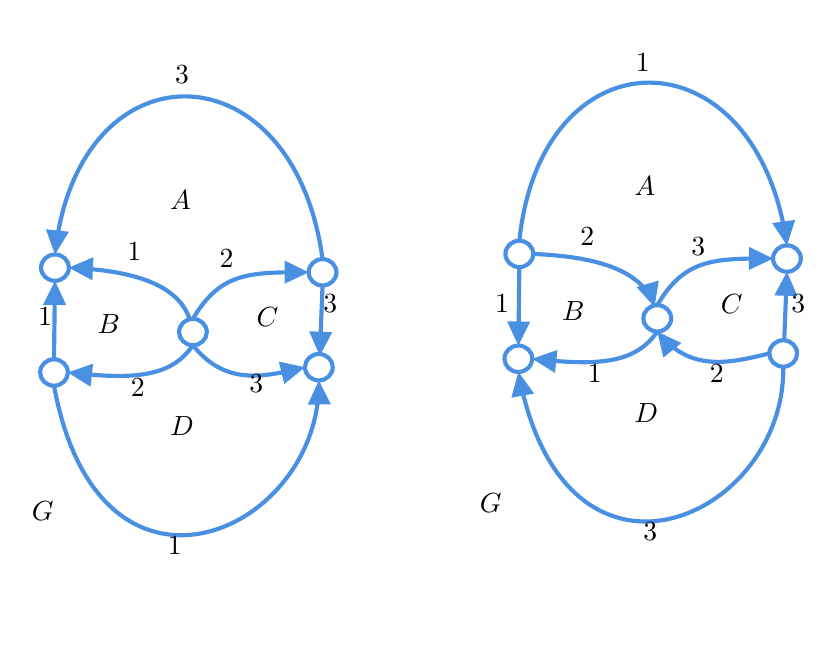
\begin{tikzpicture}[x=0.75pt,y=0.75pt,yscale=-1,xscale=1]
%uncomment if require: \path (0,877); %set diagram left start at 0, and has height of 877

%Straight Lines [id:da9943610350622754] 
\draw [color={rgb, 255:red, 74; green, 144; blue, 226 }  ,draw opacity=1 ][line width=1.5]    (143.18,155.15) -- (143.59,121.34) ;
\draw [shift={(143.64,117.34)}, rotate = 90.69] [fill={rgb, 255:red, 74; green, 144; blue, 226 }  ,fill opacity=1 ][line width=0.08]  [draw opacity=0] (11.61,-5.58) -- (0,0) -- (11.61,5.58) -- cycle    ;
%Straight Lines [id:da28864384570380464] 
\draw [color={rgb, 255:red, 74; green, 144; blue, 226 }  ,draw opacity=1 ][line width=1.5]    (272.57,119.58) -- (271.39,149.46) ;
\draw [shift={(271.23,153.46)}, rotate = 272.26] [fill={rgb, 255:red, 74; green, 144; blue, 226 }  ,fill opacity=1 ][line width=0.08]  [draw opacity=0] (11.61,-5.58) -- (0,0) -- (11.61,5.58) -- cycle    ;
%Shape: Ellipse [id:dp029827328935257524] 
\draw  [color={rgb, 255:red, 74; green, 144; blue, 226 }  ,draw opacity=1 ][fill={rgb, 255:red, 255; green, 255; blue, 255 }  ,fill opacity=1 ][line width=1.5]  (136.95,110.99) .. controls (136.95,107.48) and (139.95,104.64) .. (143.64,104.64) .. controls (147.34,104.64) and (150.33,107.48) .. (150.33,110.99) .. controls (150.33,114.5) and (147.34,117.34) .. (143.64,117.34) .. controls (139.95,117.34) and (136.95,114.5) .. (136.95,110.99) -- cycle ;
%Shape: Ellipse [id:dp4202696786928657] 
\draw  [color={rgb, 255:red, 74; green, 144; blue, 226 }  ,draw opacity=1 ][fill={rgb, 255:red, 255; green, 255; blue, 255 }  ,fill opacity=1 ][line width=1.5]  (136.49,161.51) .. controls (136.49,158) and (139.49,155.15) .. (143.18,155.15) .. controls (146.88,155.15) and (149.88,158) .. (149.88,161.51) .. controls (149.88,165.01) and (146.88,167.86) .. (143.18,167.86) .. controls (139.49,167.86) and (136.49,165.01) .. (136.49,161.51) -- cycle ;
%Shape: Ellipse [id:dp7878916678981432] 
\draw  [color={rgb, 255:red, 74; green, 144; blue, 226 }  ,draw opacity=1 ][fill={rgb, 255:red, 255; green, 255; blue, 255 }  ,fill opacity=1 ][line width=1.5]  (203.42,142.03) .. controls (203.42,138.52) and (206.41,135.67) .. (210.11,135.67) .. controls (213.8,135.67) and (216.8,138.52) .. (216.8,142.03) .. controls (216.8,145.53) and (213.8,148.38) .. (210.11,148.38) .. controls (206.41,148.38) and (203.42,145.53) .. (203.42,142.03) -- cycle ;
%Shape: Ellipse [id:dp9437208822572988] 
\draw  [color={rgb, 255:red, 74; green, 144; blue, 226 }  ,draw opacity=1 ][fill={rgb, 255:red, 255; green, 255; blue, 255 }  ,fill opacity=1 ][line width=1.5]  (265.88,113.23) .. controls (265.88,109.72) and (268.87,106.88) .. (272.57,106.88) .. controls (276.27,106.88) and (279.26,109.72) .. (279.26,113.23) .. controls (279.26,116.74) and (276.27,119.58) .. (272.57,119.58) .. controls (268.87,119.58) and (265.88,116.74) .. (265.88,113.23) -- cycle ;
%Shape: Ellipse [id:dp06226933559817249] 
\draw  [color={rgb, 255:red, 74; green, 144; blue, 226 }  ,draw opacity=1 ][fill={rgb, 255:red, 255; green, 255; blue, 255 }  ,fill opacity=1 ][line width=1.5]  (264.09,158.96) .. controls (264.09,155.46) and (267.09,152.61) .. (270.78,152.61) .. controls (274.48,152.61) and (277.48,155.46) .. (277.48,158.96) .. controls (277.48,162.47) and (274.48,165.32) .. (270.78,165.32) .. controls (267.09,165.32) and (264.09,162.47) .. (264.09,158.96) -- cycle ;
%Curve Lines [id:da2979171995828367] 
\draw [color={rgb, 255:red, 74; green, 144; blue, 226 }  ,draw opacity=1 ][line width=1.5]    (144.19,100.11) .. controls (157.44,2.47) and (258.65,4.55) .. (272.57,106.88) ;
\draw [shift={(143.64,104.64)}, rotate = 275.97] [fill={rgb, 255:red, 74; green, 144; blue, 226 }  ,fill opacity=1 ][line width=0.08]  [draw opacity=0] (11.61,-5.58) -- (0,0) -- (11.61,5.58) -- cycle    ;
%Curve Lines [id:da8764254520788726] 
\draw [color={rgb, 255:red, 74; green, 144; blue, 226 }  ,draw opacity=1 ][line width=1.5]    (154.59,111.21) .. controls (175.51,112.49) and (202.93,116.86) .. (208.77,136.52) ;
\draw [shift={(150.33,110.99)}, rotate = 2.62] [fill={rgb, 255:red, 74; green, 144; blue, 226 }  ,fill opacity=1 ][line width=0.08]  [draw opacity=0] (11.61,-5.58) -- (0,0) -- (11.61,5.58) -- cycle    ;
%Curve Lines [id:da9659495047647262] 
\draw [color={rgb, 255:red, 74; green, 144; blue, 226 }  ,draw opacity=1 ][line width=1.5]    (143.18,167.86) .. controls (164.72,285.2) and (268.93,239.85) .. (270.77,168.59) ;
\draw [shift={(270.78,165.32)}, rotate = 88.95] [fill={rgb, 255:red, 74; green, 144; blue, 226 }  ,fill opacity=1 ][line width=0.08]  [draw opacity=0] (11.61,-5.58) -- (0,0) -- (11.61,5.58) -- cycle    ;
%Curve Lines [id:da5397459745235432] 
\draw [color={rgb, 255:red, 74; green, 144; blue, 226 }  ,draw opacity=1 ][line width=1.5]    (210.11,148.38) .. controls (199.97,163.28) and (183.12,164.92) .. (153.63,161.91) ;
\draw [shift={(149.88,161.51)}, rotate = 6.33] [fill={rgb, 255:red, 74; green, 144; blue, 226 }  ,fill opacity=1 ][line width=0.08]  [draw opacity=0] (11.61,-5.58) -- (0,0) -- (11.61,5.58) -- cycle    ;
%Curve Lines [id:da4211882280413548] 
\draw [color={rgb, 255:red, 74; green, 144; blue, 226 }  ,draw opacity=1 ][line width=1.5]    (210.11,135.67) .. controls (222.75,114.11) and (236.34,113.14) .. (262.15,113.22) ;
\draw [shift={(265.88,113.23)}, rotate = 180.29] [fill={rgb, 255:red, 74; green, 144; blue, 226 }  ,fill opacity=1 ][line width=0.08]  [draw opacity=0] (11.61,-5.58) -- (0,0) -- (11.61,5.58) -- cycle    ;
%Curve Lines [id:da956839943660936] 
\draw [color={rgb, 255:red, 74; green, 144; blue, 226 }  ,draw opacity=1 ][line width=1.5]    (260.12,159.91) .. controls (241.26,164.32) and (224.71,166.59) .. (210.11,148.38) ;
\draw [shift={(264.09,158.96)}, rotate = 166.47] [fill={rgb, 255:red, 74; green, 144; blue, 226 }  ,fill opacity=1 ][line width=0.08]  [draw opacity=0] (11.61,-5.58) -- (0,0) -- (11.61,5.58) -- cycle    ;
%Straight Lines [id:da7109511854568149] 
\draw [color={rgb, 255:red, 74; green, 144; blue, 226 }  ,draw opacity=1 ][line width=1.5]    (366.97,144.53) -- (367.38,110.72) ;
\draw [shift={(366.92,148.53)}, rotate = 270.69] [fill={rgb, 255:red, 74; green, 144; blue, 226 }  ,fill opacity=1 ][line width=0.08]  [draw opacity=0] (11.61,-5.58) -- (0,0) -- (11.61,5.58) -- cycle    ;
%Straight Lines [id:da49493506455500713] 
\draw [color={rgb, 255:red, 74; green, 144; blue, 226 }  ,draw opacity=1 ][line width=1.5]    (496.15,116.96) -- (494.97,146.84) ;
\draw [shift={(496.31,112.96)}, rotate = 92.26] [fill={rgb, 255:red, 74; green, 144; blue, 226 }  ,fill opacity=1 ][line width=0.08]  [draw opacity=0] (11.61,-5.58) -- (0,0) -- (11.61,5.58) -- cycle    ;
%Shape: Ellipse [id:dp9403539709464994] 
\draw  [color={rgb, 255:red, 74; green, 144; blue, 226 }  ,draw opacity=1 ][fill={rgb, 255:red, 255; green, 255; blue, 255 }  ,fill opacity=1 ][line width=1.5]  (360.69,104.37) .. controls (360.69,100.86) and (363.68,98.02) .. (367.38,98.02) .. controls (371.08,98.02) and (374.07,100.86) .. (374.07,104.37) .. controls (374.07,107.88) and (371.08,110.72) .. (367.38,110.72) .. controls (363.68,110.72) and (360.69,107.88) .. (360.69,104.37) -- cycle ;
%Shape: Ellipse [id:dp9543762925369562] 
\draw  [color={rgb, 255:red, 74; green, 144; blue, 226 }  ,draw opacity=1 ][fill={rgb, 255:red, 255; green, 255; blue, 255 }  ,fill opacity=1 ][line width=1.5]  (360.23,154.89) .. controls (360.23,151.38) and (363.23,148.53) .. (366.92,148.53) .. controls (370.62,148.53) and (373.62,151.38) .. (373.62,154.89) .. controls (373.62,158.39) and (370.62,161.24) .. (366.92,161.24) .. controls (363.23,161.24) and (360.23,158.39) .. (360.23,154.89) -- cycle ;
%Shape: Ellipse [id:dp6094250043745837] 
\draw  [color={rgb, 255:red, 74; green, 144; blue, 226 }  ,draw opacity=1 ][fill={rgb, 255:red, 255; green, 255; blue, 255 }  ,fill opacity=1 ][line width=1.5]  (427.15,135.41) .. controls (427.15,131.9) and (430.15,129.06) .. (433.85,129.06) .. controls (437.54,129.06) and (440.54,131.9) .. (440.54,135.41) .. controls (440.54,138.92) and (437.54,141.76) .. (433.85,141.76) .. controls (430.15,141.76) and (427.15,138.92) .. (427.15,135.41) -- cycle ;
%Shape: Ellipse [id:dp7048265837255207] 
\draw  [color={rgb, 255:red, 74; green, 144; blue, 226 }  ,draw opacity=1 ][fill={rgb, 255:red, 255; green, 255; blue, 255 }  ,fill opacity=1 ][line width=1.5]  (489.62,106.61) .. controls (489.62,103.1) and (492.61,100.26) .. (496.31,100.26) .. controls (500,100.26) and (503,103.1) .. (503,106.61) .. controls (503,110.12) and (500,112.96) .. (496.31,112.96) .. controls (492.61,112.96) and (489.62,110.12) .. (489.62,106.61) -- cycle ;
%Shape: Ellipse [id:dp8750927184704229] 
\draw  [color={rgb, 255:red, 74; green, 144; blue, 226 }  ,draw opacity=1 ][fill={rgb, 255:red, 255; green, 255; blue, 255 }  ,fill opacity=1 ][line width=1.5]  (487.83,152.35) .. controls (487.83,148.84) and (490.83,145.99) .. (494.52,145.99) .. controls (498.22,145.99) and (501.22,148.84) .. (501.22,152.35) .. controls (501.22,155.85) and (498.22,158.7) .. (494.52,158.7) .. controls (490.83,158.7) and (487.83,155.85) .. (487.83,152.35) -- cycle ;
%Curve Lines [id:da5236484284848602] 
\draw [color={rgb, 255:red, 74; green, 144; blue, 226 }  ,draw opacity=1 ][line width=1.5]    (367.38,98.02) .. controls (377.97,-3.17) and (480.11,-3.63) .. (495.86,97.17) ;
\draw [shift={(496.31,100.26)}, rotate = 262.26] [fill={rgb, 255:red, 74; green, 144; blue, 226 }  ,fill opacity=1 ][line width=0.08]  [draw opacity=0] (11.61,-5.58) -- (0,0) -- (11.61,5.58) -- cycle    ;
%Curve Lines [id:da9662673859391505] 
\draw [color={rgb, 255:red, 74; green, 144; blue, 226 }  ,draw opacity=1 ][line width=1.5]    (374.07,104.37) .. controls (394.05,105.28) and (422.58,108.46) .. (431.12,126.3) ;
\draw [shift={(432.51,129.9)}, rotate = 253.46] [fill={rgb, 255:red, 74; green, 144; blue, 226 }  ,fill opacity=1 ][line width=0.08]  [draw opacity=0] (11.61,-5.58) -- (0,0) -- (11.61,5.58) -- cycle    ;
%Curve Lines [id:da48834267482785687] 
\draw [color={rgb, 255:red, 74; green, 144; blue, 226 }  ,draw opacity=1 ][line width=1.5]    (367.96,166.49) .. controls (391.97,278.91) and (495.84,230.72) .. (494.52,158.7) ;
\draw [shift={(366.92,161.24)}, rotate = 79.6] [fill={rgb, 255:red, 74; green, 144; blue, 226 }  ,fill opacity=1 ][line width=0.08]  [draw opacity=0] (11.61,-5.58) -- (0,0) -- (11.61,5.58) -- cycle    ;
%Curve Lines [id:da8150566103908512] 
\draw [color={rgb, 255:red, 74; green, 144; blue, 226 }  ,draw opacity=1 ][line width=1.5]    (433.85,141.76) .. controls (423.71,156.66) and (406.86,158.3) .. (377.37,155.29) ;
\draw [shift={(373.62,154.89)}, rotate = 6.33] [fill={rgb, 255:red, 74; green, 144; blue, 226 }  ,fill opacity=1 ][line width=0.08]  [draw opacity=0] (11.61,-5.58) -- (0,0) -- (11.61,5.58) -- cycle    ;
%Curve Lines [id:da4757930219164036] 
\draw [color={rgb, 255:red, 74; green, 144; blue, 226 }  ,draw opacity=1 ][line width=1.5]    (433.85,129.06) .. controls (446.49,107.49) and (460.08,106.52) .. (485.88,106.6) ;
\draw [shift={(489.62,106.61)}, rotate = 180.29] [fill={rgb, 255:red, 74; green, 144; blue, 226 }  ,fill opacity=1 ][line width=0.08]  [draw opacity=0] (11.61,-5.58) -- (0,0) -- (11.61,5.58) -- cycle    ;
%Curve Lines [id:da9886701870479793] 
\draw [color={rgb, 255:red, 74; green, 144; blue, 226 }  ,draw opacity=1 ][line width=1.5]    (487.83,152.35) .. controls (468.44,157.01) and (451.43,160.8) .. (436.44,144.76) ;
\draw [shift={(433.85,141.76)}, rotate = 51.28] [fill={rgb, 255:red, 74; green, 144; blue, 226 }  ,fill opacity=1 ][line width=0.08]  [draw opacity=0] (11.61,-5.58) -- (0,0) -- (11.61,5.58) -- cycle    ;

% Text Node
\draw (197.61,72.18) node [anchor=north west][inner sep=0.75pt]    {$A$};
% Text Node
\draw (162.72,132.26) node [anchor=north west][inner sep=0.75pt]    {$B$};
% Text Node
\draw (239.25,128.92) node [anchor=north west][inner sep=0.75pt]    {$C$};
% Text Node
\draw (197.61,181.41) node [anchor=north west][inner sep=0.75pt]    {$D$};
% Text Node
\draw (196.52,239.02) node [anchor=north west][inner sep=0.75pt]    {$1$};
% Text Node
\draw (221.51,100.97) node [anchor=north west][inner sep=0.75pt]    {$2$};
% Text Node
\draw (200.09,12.4) node [anchor=north west][inner sep=0.75pt]    {$3$};
% Text Node
\draw (235.78,161.1) node [anchor=north west][inner sep=0.75pt]    {$3$};
% Text Node
\draw (177,97.4) node [anchor=north west][inner sep=0.75pt]    {$1$};
% Text Node
\draw (134.06,128.92) node [anchor=north west][inner sep=0.75pt]    {$1$};
% Text Node
\draw (178.68,162.8) node [anchor=north west][inner sep=0.75pt]    {$2$};
% Text Node
\draw (271.48,122.5) node [anchor=north west][inner sep=0.75pt]    {$3$};
% Text Node
\draw (421.34,65.56) node [anchor=north west][inner sep=0.75pt]    {$A$};
% Text Node
\draw (386.46,125.64) node [anchor=north west][inner sep=0.75pt]    {$B$};
% Text Node
\draw (462.98,122.3) node [anchor=north west][inner sep=0.75pt]    {$C$};
% Text Node
\draw (421.34,174.79) node [anchor=north west][inner sep=0.75pt]    {$D$};
% Text Node
\draw (354.23,122.3) node [anchor=north west][inner sep=0.75pt]    {$1$};
% Text Node
\draw (398.85,156.18) node [anchor=north west][inner sep=0.75pt]    {$1$};
% Text Node
\draw (395.28,90.12) node [anchor=north west][inner sep=0.75pt]    {$2$};
% Text Node
\draw (497,122.3) node [anchor=north west][inner sep=0.75pt]    {$3$};
% Text Node
\draw (422.05,6.28) node [anchor=north west][inner sep=0.75pt]    {$1$};
% Text Node
\draw (457.74,156.18) node [anchor=north west][inner sep=0.75pt]    {$2$};
% Text Node
\draw (425.62,232.4) node [anchor=north west][inner sep=0.75pt]    {$3$};
% Text Node
\draw (448.82,95.2) node [anchor=north west][inner sep=0.75pt]    {$3$};
% Text Node
\draw (131,222.4) node [anchor=north west][inner sep=0.75pt]    {$G$};
% Text Node
\draw (346.85,218.4) node [anchor=north west][inner sep=0.75pt]    {$G$};


\end{tikzpicture}
        \caption{dos pirámides ideales del enlace de Whitehead}
    \end{figure}
\end{eg}
\begin{eg}
    Considere la siguiente proyeccion del nudo $6_1$ que no es precisamente la estandar mas tiene un parecido con la proyeccion del nudo de 8 y por eso la tomamos
    \begin{figure}[H]
    \centering
    %!TEX root = ./main.tex



\tikzset{every picture/.style={line width=0.75pt}} %set default line width to 0.75pt        

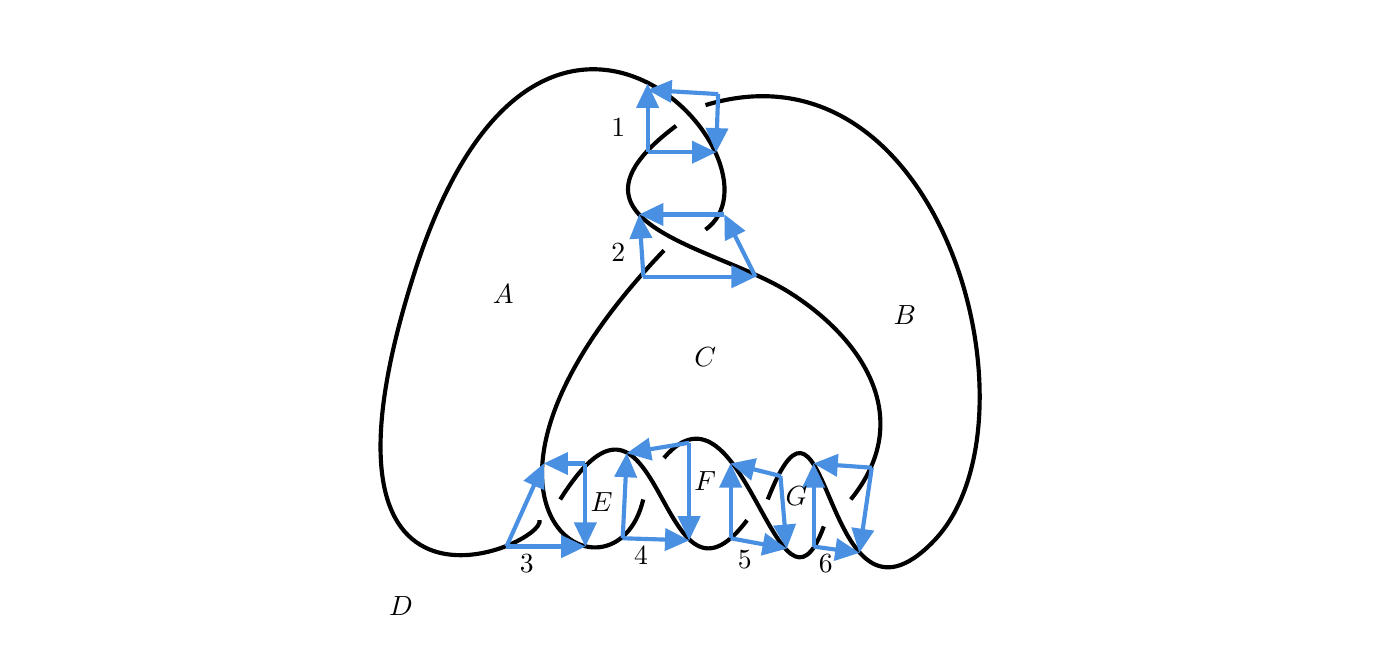
\begin{tikzpicture}[x=0.75pt,y=0.75pt,yscale=-1,xscale=1]
%uncomment if require: \path (0,877); %set diagram left start at 0, and has height of 877
\path[use as bounding box] (20,10) rectangle (660,300);
%Curve Lines [id:da7624936084054103] 
\draw [line width=1.5]    (332.42,57.3) .. controls (269.42,104.3) and (350.91,114.97) .. (386.58,137.3) .. controls (422.25,159.64) and (448.25,198.3) .. (416.58,237.3) ;
%Curve Lines [id:da19391436252011207] 
\draw [line width=1.5]    (316.58,237.3) .. controls (302.91,294.97) and (208.25,240.97) .. (326.58,117.3) ;
%Curve Lines [id:da04931308389248612] 
\draw [line width=1.5]    (276.58,237.3) .. controls (326.25,158.3) and (323.58,304.3) .. (366.58,247.3) ;
%Curve Lines [id:da7925895816985254] 
\draw [line width=1.5]    (346.58,107.3) .. controls (390.25,75.64) and (266.91,-60.36) .. (206.58,127.3) .. controls (146.25,314.97) and (270.25,258.97) .. (266.58,247.3) ;
%Curve Lines [id:da7432199945489849] 
\draw [line width=1.5]    (376.58,237.3) .. controls (406.91,159.64) and (402.25,313.64) .. (456.58,257.3) .. controls (510.91,200.97) and (461.58,12.3) .. (346.58,47.3) ;
%Curve Lines [id:da5685625074522969] 
\draw [line width=1.5]    (326.58,217.3) .. controls (364.91,172.3) and (381.91,308.97) .. (403.58,250.3) ;
%Straight Lines [id:da1141281197725319] 
\draw [color={rgb, 255:red, 74; green, 144; blue, 226 }  ,draw opacity=1 ][line width=1.5]    (318.68,70) -- (347.68,70) ;
\draw [shift={(351.68,70)}, rotate = 180] [fill={rgb, 255:red, 74; green, 144; blue, 226 }  ,fill opacity=1 ][line width=0.08]  [draw opacity=0] (11.61,-5.58) -- (0,0) -- (11.61,5.58) -- cycle    ;
%Straight Lines [id:da5128754818859278] 
\draw [color={rgb, 255:red, 74; green, 144; blue, 226 }  ,draw opacity=1 ][line width=1.5]    (318.68,70) -- (318.68,41) ;
\draw [shift={(318.68,37)}, rotate = 90] [fill={rgb, 255:red, 74; green, 144; blue, 226 }  ,fill opacity=1 ][line width=0.08]  [draw opacity=0] (11.61,-5.58) -- (0,0) -- (11.61,5.58) -- cycle    ;
%Straight Lines [id:da6937466521525161] 
\draw [color={rgb, 255:red, 74; green, 144; blue, 226 }  ,draw opacity=1 ][line width=1.5]    (352.68,42) -- (351.82,66) ;
\draw [shift={(351.68,70)}, rotate = 272.05] [fill={rgb, 255:red, 74; green, 144; blue, 226 }  ,fill opacity=1 ][line width=0.08]  [draw opacity=0] (11.61,-5.58) -- (0,0) -- (11.61,5.58) -- cycle    ;
%Straight Lines [id:da1076986821814464] 
\draw [color={rgb, 255:red, 74; green, 144; blue, 226 }  ,draw opacity=1 ][line width=1.5]    (352.68,42) -- (322.67,40.23) ;
\draw [shift={(318.68,40)}, rotate = 3.37] [fill={rgb, 255:red, 74; green, 144; blue, 226 }  ,fill opacity=1 ][line width=0.08]  [draw opacity=0] (11.61,-5.58) -- (0,0) -- (11.61,5.58) -- cycle    ;
%Straight Lines [id:da5957859563126462] 
\draw [color={rgb, 255:red, 74; green, 144; blue, 226 }  ,draw opacity=1 ][line width=1.5]    (355.68,100) -- (318.68,100) ;
\draw [shift={(314.68,100)}, rotate = 360] [fill={rgb, 255:red, 74; green, 144; blue, 226 }  ,fill opacity=1 ][line width=0.08]  [draw opacity=0] (11.61,-5.58) -- (0,0) -- (11.61,5.58) -- cycle    ;
%Straight Lines [id:da6302195089744549] 
\draw [color={rgb, 255:red, 74; green, 144; blue, 226 }  ,draw opacity=1 ][line width=1.5]    (316.68,130) -- (366.68,130) ;
\draw [shift={(370.68,130)}, rotate = 180] [fill={rgb, 255:red, 74; green, 144; blue, 226 }  ,fill opacity=1 ][line width=0.08]  [draw opacity=0] (11.61,-5.58) -- (0,0) -- (11.61,5.58) -- cycle    ;
%Straight Lines [id:da5412838641193578] 
\draw [color={rgb, 255:red, 74; green, 144; blue, 226 }  ,draw opacity=1 ][line width=1.5]    (316.68,130) -- (314.94,103.99) ;
\draw [shift={(314.68,100)}, rotate = 86.19] [fill={rgb, 255:red, 74; green, 144; blue, 226 }  ,fill opacity=1 ][line width=0.08]  [draw opacity=0] (11.61,-5.58) -- (0,0) -- (11.61,5.58) -- cycle    ;
%Straight Lines [id:da3701320323663966] 
\draw [color={rgb, 255:red, 74; green, 144; blue, 226 }  ,draw opacity=1 ][line width=1.5]    (370.68,130) -- (357.47,103.58) ;
\draw [shift={(355.68,100)}, rotate = 63.43] [fill={rgb, 255:red, 74; green, 144; blue, 226 }  ,fill opacity=1 ][line width=0.08]  [draw opacity=0] (11.61,-5.58) -- (0,0) -- (11.61,5.58) -- cycle    ;
%Straight Lines [id:da4037972105202199] 
\draw [color={rgb, 255:red, 74; green, 144; blue, 226 }  ,draw opacity=1 ][line width=1.5]    (250.68,260) -- (267.04,223.65) ;
\draw [shift={(268.68,220)}, rotate = 114.23] [fill={rgb, 255:red, 74; green, 144; blue, 226 }  ,fill opacity=1 ][line width=0.08]  [draw opacity=0] (11.61,-5.58) -- (0,0) -- (11.61,5.58) -- cycle    ;
%Straight Lines [id:da8718338183932847] 
\draw [color={rgb, 255:red, 74; green, 144; blue, 226 }  ,draw opacity=1 ][line width=1.5]    (288.68,220) -- (288.68,256) ;
\draw [shift={(288.68,260)}, rotate = 270] [fill={rgb, 255:red, 74; green, 144; blue, 226 }  ,fill opacity=1 ][line width=0.08]  [draw opacity=0] (11.61,-5.58) -- (0,0) -- (11.61,5.58) -- cycle    ;
%Straight Lines [id:da7553369000057689] 
\draw [color={rgb, 255:red, 74; green, 144; blue, 226 }  ,draw opacity=1 ][line width=1.5]    (306.68,256) -- (308.48,219) ;
\draw [shift={(308.68,215)}, rotate = 92.79] [fill={rgb, 255:red, 74; green, 144; blue, 226 }  ,fill opacity=1 ][line width=0.08]  [draw opacity=0] (11.61,-5.58) -- (0,0) -- (11.61,5.58) -- cycle    ;
%Straight Lines [id:da7979498405597526] 
\draw [color={rgb, 255:red, 74; green, 144; blue, 226 }  ,draw opacity=1 ][line width=1.5]    (338.68,210) -- (338.68,253) ;
\draw [shift={(338.68,257)}, rotate = 270] [fill={rgb, 255:red, 74; green, 144; blue, 226 }  ,fill opacity=1 ][line width=0.08]  [draw opacity=0] (11.61,-5.58) -- (0,0) -- (11.61,5.58) -- cycle    ;
%Straight Lines [id:da9990695315517517] 
\draw [color={rgb, 255:red, 74; green, 144; blue, 226 }  ,draw opacity=1 ][line width=1.5]    (358.68,256) -- (358.68,224) ;
\draw [shift={(358.68,220)}, rotate = 90] [fill={rgb, 255:red, 74; green, 144; blue, 226 }  ,fill opacity=1 ][line width=0.08]  [draw opacity=0] (11.61,-5.58) -- (0,0) -- (11.61,5.58) -- cycle    ;
%Straight Lines [id:da5789283453234753] 
\draw [color={rgb, 255:red, 74; green, 144; blue, 226 }  ,draw opacity=1 ][line width=1.5]    (382.68,226) -- (385.34,257.01) ;
\draw [shift={(385.68,261)}, rotate = 265.1] [fill={rgb, 255:red, 74; green, 144; blue, 226 }  ,fill opacity=1 ][line width=0.08]  [draw opacity=0] (11.61,-5.58) -- (0,0) -- (11.61,5.58) -- cycle    ;
%Straight Lines [id:da8699663998653359] 
\draw [color={rgb, 255:red, 74; green, 144; blue, 226 }  ,draw opacity=1 ][line width=1.5]    (398.68,260) -- (398.68,224) ;
\draw [shift={(398.68,220)}, rotate = 90] [fill={rgb, 255:red, 74; green, 144; blue, 226 }  ,fill opacity=1 ][line width=0.08]  [draw opacity=0] (11.61,-5.58) -- (0,0) -- (11.61,5.58) -- cycle    ;
%Straight Lines [id:da798656100582777] 
\draw [color={rgb, 255:red, 74; green, 144; blue, 226 }  ,draw opacity=1 ][line width=1.5]    (426.68,222) -- (421.26,259.04) ;
\draw [shift={(420.68,263)}, rotate = 278.33] [fill={rgb, 255:red, 74; green, 144; blue, 226 }  ,fill opacity=1 ][line width=0.08]  [draw opacity=0] (11.61,-5.58) -- (0,0) -- (11.61,5.58) -- cycle    ;
%Straight Lines [id:da33279694069000054] 
\draw [color={rgb, 255:red, 74; green, 144; blue, 226 }  ,draw opacity=1 ][line width=1.5]    (288.68,220) -- (272.68,220) ;
\draw [shift={(268.68,220)}, rotate = 360] [fill={rgb, 255:red, 74; green, 144; blue, 226 }  ,fill opacity=1 ][line width=0.08]  [draw opacity=0] (11.61,-5.58) -- (0,0) -- (11.61,5.58) -- cycle    ;
%Straight Lines [id:da43289558059406263] 
\draw [color={rgb, 255:red, 74; green, 144; blue, 226 }  ,draw opacity=1 ][line width=1.5]    (338.68,210) -- (312.62,214.34) ;
\draw [shift={(308.68,215)}, rotate = 350.54] [fill={rgb, 255:red, 74; green, 144; blue, 226 }  ,fill opacity=1 ][line width=0.08]  [draw opacity=0] (11.61,-5.58) -- (0,0) -- (11.61,5.58) -- cycle    ;
%Straight Lines [id:da6303991823506472] 
\draw [color={rgb, 255:red, 74; green, 144; blue, 226 }  ,draw opacity=1 ][line width=1.5]    (382.68,226) -- (362.56,220.97) ;
\draw [shift={(358.68,220)}, rotate = 14.04] [fill={rgb, 255:red, 74; green, 144; blue, 226 }  ,fill opacity=1 ][line width=0.08]  [draw opacity=0] (11.61,-5.58) -- (0,0) -- (11.61,5.58) -- cycle    ;
%Straight Lines [id:da8930356844444237] 
\draw [color={rgb, 255:red, 74; green, 144; blue, 226 }  ,draw opacity=1 ][line width=1.5]    (426.68,222) -- (402.67,220.28) ;
\draw [shift={(398.68,220)}, rotate = 4.09] [fill={rgb, 255:red, 74; green, 144; blue, 226 }  ,fill opacity=1 ][line width=0.08]  [draw opacity=0] (11.61,-5.58) -- (0,0) -- (11.61,5.58) -- cycle    ;
%Straight Lines [id:da9121806098865429] 
\draw [color={rgb, 255:red, 74; green, 144; blue, 226 }  ,draw opacity=1 ][line width=1.5]    (250.68,260) -- (284.68,260) ;
\draw [shift={(288.68,260)}, rotate = 180] [fill={rgb, 255:red, 74; green, 144; blue, 226 }  ,fill opacity=1 ][line width=0.08]  [draw opacity=0] (11.61,-5.58) -- (0,0) -- (11.61,5.58) -- cycle    ;
%Straight Lines [id:da632074891050223] 
\draw [color={rgb, 255:red, 74; green, 144; blue, 226 }  ,draw opacity=1 ][line width=1.5]    (306.68,256) -- (334.68,256.88) ;
\draw [shift={(338.68,257)}, rotate = 181.79] [fill={rgb, 255:red, 74; green, 144; blue, 226 }  ,fill opacity=1 ][line width=0.08]  [draw opacity=0] (11.61,-5.58) -- (0,0) -- (11.61,5.58) -- cycle    ;
%Straight Lines [id:da7854913192561737] 
\draw [color={rgb, 255:red, 74; green, 144; blue, 226 }  ,draw opacity=1 ][line width=1.5]    (358.68,256) -- (381.74,260.27) ;
\draw [shift={(385.68,261)}, rotate = 190.49] [fill={rgb, 255:red, 74; green, 144; blue, 226 }  ,fill opacity=1 ][line width=0.08]  [draw opacity=0] (11.61,-5.58) -- (0,0) -- (11.61,5.58) -- cycle    ;
%Straight Lines [id:da3077701960838797] 
\draw [color={rgb, 255:red, 74; green, 144; blue, 226 }  ,draw opacity=1 ][line width=1.5]    (398.68,260) -- (416.71,262.46) ;
\draw [shift={(420.68,263)}, rotate = 187.77] [fill={rgb, 255:red, 74; green, 144; blue, 226 }  ,fill opacity=1 ][line width=0.08]  [draw opacity=0] (11.61,-5.58) -- (0,0) -- (11.61,5.58) -- cycle    ;

% Text Node
\draw (242.68,132.4) node [anchor=north west][inner sep=0.75pt]    {$A$};
% Text Node
\draw (435.68,142.4) node [anchor=north west][inner sep=0.75pt]    {$B$};
% Text Node
\draw (339.68,162.4) node [anchor=north west][inner sep=0.75pt]    {$C$};
% Text Node
\draw (192.68,282.4) node [anchor=north west][inner sep=0.75pt]    {$D$};
% Text Node
\draw (289.68,232.4) node [anchor=north west][inner sep=0.75pt]    {$E$};
% Text Node
\draw (339.68,222.4) node [anchor=north west][inner sep=0.75pt]    {$F$};
% Text Node
\draw (383.68,229.4) node [anchor=north west][inner sep=0.75pt]    {$G$};
% Text Node
\draw (299.68,52.4) node [anchor=north west][inner sep=0.75pt]    {$1$};
% Text Node
\draw (299.68,112.4) node [anchor=north west][inner sep=0.75pt]    {$2$};
% Text Node
\draw (255.68,262.4) node [anchor=north west][inner sep=0.75pt]    {$3$};
% Text Node
\draw (310.68,258.4) node [anchor=north west][inner sep=0.75pt]    {$4$};
% Text Node
\draw (360.68,260.4) node [anchor=north west][inner sep=0.75pt]    {$5$};
% Text Node
\draw (399.68,262.4) node [anchor=north west][inner sep=0.75pt]    {$6$};


\end{tikzpicture}
        \caption{Nudo $6_1$}
    \end{figure}
   Nuevamente por los pasos de antes obtenemos los siguientes diagramas que nos dan ambos poliedros, el de arriba visto desde adentro y el de abajo visto desde afuera.
    \begin{figure}[H]
    %!TEX root = ./main.tex



\tikzset{every picture/.style={line width=0.75pt}} %set default line width to 0.75pt        

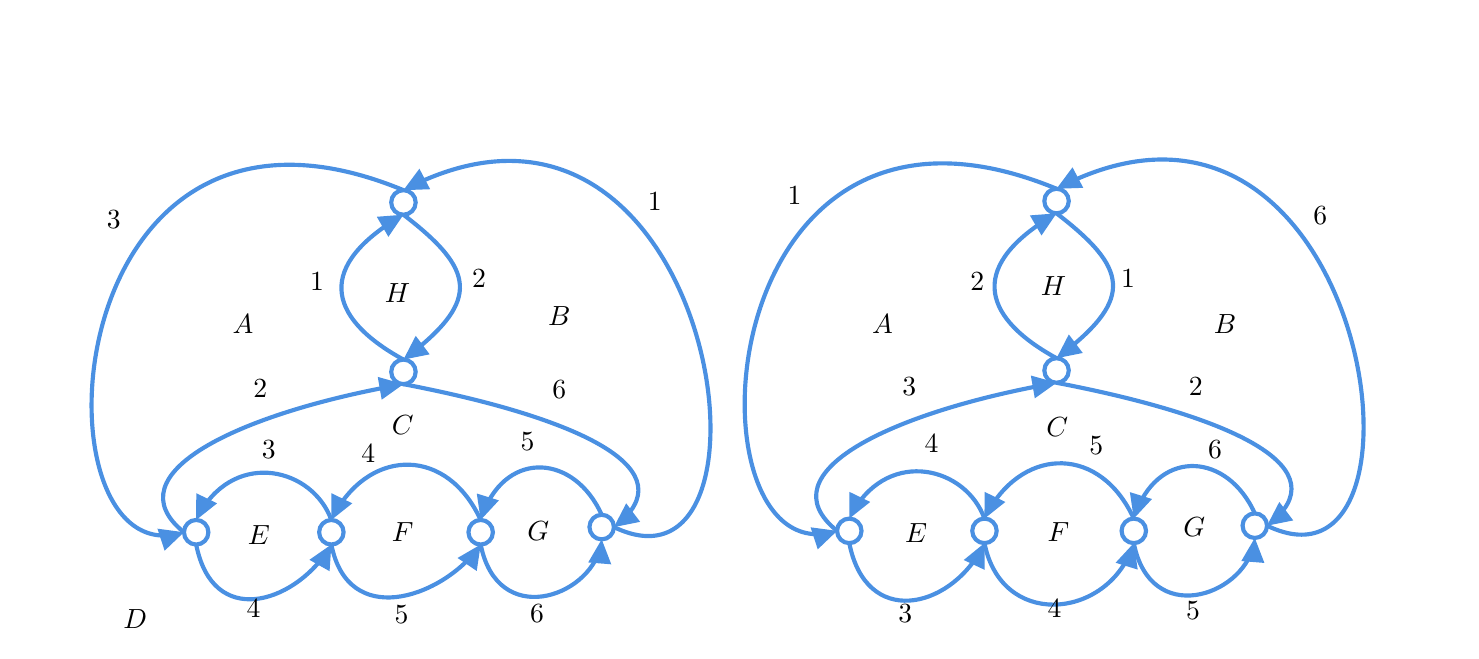
\begin{tikzpicture}[x=0.75pt,y=0.75pt,yscale=-1,xscale=1]
%uncomment if require: \path (0,877); %set diagram left start at 0, and has height of 877

%Shape: Ellipse [id:dp2062482206131232] 
\draw  [color={rgb, 255:red, 74; green, 144; blue, 226 }  ,draw opacity=1 ][line width=1.5]  (181.18,43.69) .. controls (181.18,40.42) and (183.82,37.77) .. (187.08,37.77) .. controls (190.33,37.77) and (192.97,40.42) .. (192.97,43.69) .. controls (192.97,46.95) and (190.33,49.6) .. (187.08,49.6) .. controls (183.82,49.6) and (181.18,46.95) .. (181.18,43.69) -- cycle ;
%Shape: Ellipse [id:dp42181631305663214] 
\draw  [color={rgb, 255:red, 74; green, 144; blue, 226 }  ,draw opacity=1 ][line width=1.5]  (181.18,125.31) .. controls (181.18,122.05) and (183.82,119.39) .. (187.08,119.39) .. controls (190.33,119.39) and (192.97,122.05) .. (192.97,125.31) .. controls (192.97,128.58) and (190.33,131.23) .. (187.08,131.23) .. controls (183.82,131.23) and (181.18,128.58) .. (181.18,125.31) -- cycle ;
%Shape: Ellipse [id:dp1893981875046039] 
\draw  [color={rgb, 255:red, 74; green, 144; blue, 226 }  ,draw opacity=1 ][line width=1.5]  (81.33,202.58) .. controls (81.33,199.31) and (83.97,196.66) .. (87.22,196.66) .. controls (90.48,196.66) and (93.11,199.31) .. (93.11,202.58) .. controls (93.11,205.85) and (90.48,208.5) .. (87.22,208.5) .. controls (83.97,208.5) and (81.33,205.85) .. (81.33,202.58) -- cycle ;
%Shape: Ellipse [id:dp3630097335542829] 
\draw  [color={rgb, 255:red, 74; green, 144; blue, 226 }  ,draw opacity=1 ][line width=1.5]  (276.69,200.09) .. controls (276.69,196.82) and (279.33,194.17) .. (282.59,194.17) .. controls (285.84,194.17) and (288.48,196.82) .. (288.48,200.09) .. controls (288.48,203.36) and (285.84,206.01) .. (282.59,206.01) .. controls (279.33,206.01) and (276.69,203.36) .. (276.69,200.09) -- cycle ;
%Shape: Ellipse [id:dp12213112120599945] 
\draw  [color={rgb, 255:red, 74; green, 144; blue, 226 }  ,draw opacity=1 ][line width=1.5]  (146.45,202.58) .. controls (146.45,199.31) and (149.09,196.66) .. (152.34,196.66) .. controls (155.6,196.66) and (158.24,199.31) .. (158.24,202.58) .. controls (158.24,205.85) and (155.6,208.5) .. (152.34,208.5) .. controls (149.09,208.5) and (146.45,205.85) .. (146.45,202.58) -- cycle ;
%Shape: Ellipse [id:dp14956651149377553] 
\draw  [color={rgb, 255:red, 74; green, 144; blue, 226 }  ,draw opacity=1 ][line width=1.5]  (218.4,202.58) .. controls (218.4,199.31) and (221.03,196.66) .. (224.29,196.66) .. controls (227.54,196.66) and (230.18,199.31) .. (230.18,202.58) .. controls (230.18,205.85) and (227.54,208.5) .. (224.29,208.5) .. controls (221.03,208.5) and (218.4,205.85) .. (218.4,202.58) -- cycle ;
%Curve Lines [id:da13558369698297235] 
\draw [color={rgb, 255:red, 74; green, 144; blue, 226 }  ,draw opacity=1 ][line width=1.5]    (190.32,116.91) .. controls (224.15,90.46) and (221.37,75.9) .. (187.08,49.6) ;
\draw [shift={(187.08,119.39)}, rotate = 323] [fill={rgb, 255:red, 74; green, 144; blue, 226 }  ,fill opacity=1 ][line width=0.08]  [draw opacity=0] (11.61,-5.58) -- (0,0) -- (11.61,5.58) -- cycle    ;
%Curve Lines [id:da08096805629350934] 
\draw [color={rgb, 255:red, 74; green, 144; blue, 226 }  ,draw opacity=1 ][line width=1.5]    (187.08,119.39) .. controls (153.21,100.86) and (142.93,76.71) .. (183.83,51.54) ;
\draw [shift={(187.08,49.6)}, rotate = 149.92] [fill={rgb, 255:red, 74; green, 144; blue, 226 }  ,fill opacity=1 ][line width=0.08]  [draw opacity=0] (11.61,-5.58) -- (0,0) -- (11.61,5.58) -- cycle    ;
%Curve Lines [id:da46118430818328493] 
\draw [color={rgb, 255:red, 74; green, 144; blue, 226 }  ,draw opacity=1 ][line width=1.5]    (81.33,202.58) .. controls (46.2,174.35) and (108.26,145.51) .. (183.62,131.85) ;
\draw [shift={(187.08,131.23)}, rotate = 170.12] [fill={rgb, 255:red, 74; green, 144; blue, 226 }  ,fill opacity=1 ][line width=0.08]  [draw opacity=0] (11.61,-5.58) -- (0,0) -- (11.61,5.58) -- cycle    ;
%Curve Lines [id:da12684350601217753] 
\draw [color={rgb, 255:red, 74; green, 144; blue, 226 }  ,draw opacity=1 ][line width=1.5]    (292.05,197.16) .. controls (321.77,170.32) and (267.27,146.57) .. (187.08,131.23) ;
\draw [shift={(288.48,200.09)}, rotate = 323] [fill={rgb, 255:red, 74; green, 144; blue, 226 }  ,fill opacity=1 ][line width=0.08]  [draw opacity=0] (11.61,-5.58) -- (0,0) -- (11.61,5.58) -- cycle    ;
%Curve Lines [id:da12533726813089074] 
\draw [color={rgb, 255:red, 74; green, 144; blue, 226 }  ,draw opacity=1 ][line width=1.5]    (288.48,200.09) .. controls (375.8,242.25) and (338.78,-38.85) .. (189.34,36.6) ;
\draw [shift={(187.08,37.77)}, rotate = 332.3] [fill={rgb, 255:red, 74; green, 144; blue, 226 }  ,fill opacity=1 ][line width=0.08]  [draw opacity=0] (11.61,-5.58) -- (0,0) -- (11.61,5.58) -- cycle    ;
%Curve Lines [id:da052098391594170956] 
\draw [color={rgb, 255:red, 74; green, 144; blue, 226 }  ,draw opacity=1 ][line width=1.5]    (76.95,203.7) .. controls (7.03,216.62) and (19.32,-31.54) .. (187.08,37.77) ;
\draw [shift={(81.33,202.58)}, rotate = 161.99] [fill={rgb, 255:red, 74; green, 144; blue, 226 }  ,fill opacity=1 ][line width=0.08]  [draw opacity=0] (11.61,-5.58) -- (0,0) -- (11.61,5.58) -- cycle    ;
%Curve Lines [id:da545296203025464] 
\draw [color={rgb, 255:red, 74; green, 144; blue, 226 }  ,draw opacity=1 ][line width=1.5]    (87.22,208.5) .. controls (95.26,249.18) and (133.74,236.79) .. (150.38,211.7) ;
\draw [shift={(152.34,208.5)}, rotate = 119.46] [fill={rgb, 255:red, 74; green, 144; blue, 226 }  ,fill opacity=1 ][line width=0.08]  [draw opacity=0] (11.61,-5.58) -- (0,0) -- (11.61,5.58) -- cycle    ;
%Curve Lines [id:da5810485905154714] 
\draw [color={rgb, 255:red, 74; green, 144; blue, 226 }  ,draw opacity=1 ][line width=1.5]    (152.34,208.5) .. controls (160.38,249.18) and (203.97,234.33) .. (222.15,211.41) ;
\draw [shift={(224.29,208.5)}, rotate = 124.16] [fill={rgb, 255:red, 74; green, 144; blue, 226 }  ,fill opacity=1 ][line width=0.08]  [draw opacity=0] (11.61,-5.58) -- (0,0) -- (11.61,5.58) -- cycle    ;
%Curve Lines [id:da14849415068653748] 
\draw [color={rgb, 255:red, 74; green, 144; blue, 226 }  ,draw opacity=1 ][line width=1.5]    (224.29,208.5) .. controls (232.28,248.97) and (276.2,234.31) .. (282.02,209.57) ;
\draw [shift={(282.59,206.01)}, rotate = 94.63] [fill={rgb, 255:red, 74; green, 144; blue, 226 }  ,fill opacity=1 ][line width=0.08]  [draw opacity=0] (11.61,-5.58) -- (0,0) -- (11.61,5.58) -- cycle    ;
%Curve Lines [id:da46264718836376073] 
\draw [color={rgb, 255:red, 74; green, 144; blue, 226 }  ,draw opacity=1 ][line width=1.5]    (89.34,192.72) .. controls (107.05,162.8) and (143.41,171.84) .. (152.34,196.66) ;
\draw [shift={(87.22,196.66)}, rotate = 295.84] [fill={rgb, 255:red, 74; green, 144; blue, 226 }  ,fill opacity=1 ][line width=0.08]  [draw opacity=0] (11.61,-5.58) -- (0,0) -- (11.61,5.58) -- cycle    ;
%Curve Lines [id:da44941926103098273] 
\draw [color={rgb, 255:red, 74; green, 144; blue, 226 }  ,draw opacity=1 ][line width=1.5]    (154.46,192.67) .. controls (172.13,161.99) and (208.21,161.67) .. (224.29,196.66) ;
\draw [shift={(152.34,196.66)}, rotate = 295.84] [fill={rgb, 255:red, 74; green, 144; blue, 226 }  ,fill opacity=1 ][line width=0.08]  [draw opacity=0] (11.61,-5.58) -- (0,0) -- (11.61,5.58) -- cycle    ;
%Curve Lines [id:da22225476038038006] 
\draw [color={rgb, 255:red, 74; green, 144; blue, 226 }  ,draw opacity=1 ][line width=1.5]    (225.66,192.76) .. controls (237.53,162.85) and (269.49,165.16) .. (282.59,194.17) ;
\draw [shift={(224.29,196.66)}, rotate = 287.25] [fill={rgb, 255:red, 74; green, 144; blue, 226 }  ,fill opacity=1 ][line width=0.08]  [draw opacity=0] (11.61,-5.58) -- (0,0) -- (11.61,5.58) -- cycle    ;
%Shape: Ellipse [id:dp42372727795787335] 
\draw  [color={rgb, 255:red, 74; green, 144; blue, 226 }  ,draw opacity=1 ][line width=1.5]  (495.85,43.02) .. controls (495.85,39.75) and (498.49,37.1) .. (501.74,37.1) .. controls (505,37.1) and (507.63,39.75) .. (507.63,43.02) .. controls (507.63,46.29) and (505,48.94) .. (501.74,48.94) .. controls (498.49,48.94) and (495.85,46.29) .. (495.85,43.02) -- cycle ;
%Shape: Ellipse [id:dp1870179348026778] 
\draw  [color={rgb, 255:red, 74; green, 144; blue, 226 }  ,draw opacity=1 ][line width=1.5]  (495.85,124.65) .. controls (495.85,121.38) and (498.49,118.73) .. (501.74,118.73) .. controls (505,118.73) and (507.63,121.38) .. (507.63,124.65) .. controls (507.63,127.92) and (505,130.57) .. (501.74,130.57) .. controls (498.49,130.57) and (495.85,127.92) .. (495.85,124.65) -- cycle ;
%Shape: Ellipse [id:dp6111256363608131] 
\draw  [color={rgb, 255:red, 74; green, 144; blue, 226 }  ,draw opacity=1 ][line width=1.5]  (396,201.92) .. controls (396,198.65) and (398.64,196) .. (401.89,196) .. controls (405.14,196) and (407.78,198.65) .. (407.78,201.92) .. controls (407.78,205.18) and (405.14,207.83) .. (401.89,207.83) .. controls (398.64,207.83) and (396,205.18) .. (396,201.92) -- cycle ;
%Shape: Ellipse [id:dp9315304169845421] 
\draw  [color={rgb, 255:red, 74; green, 144; blue, 226 }  ,draw opacity=1 ][line width=1.5]  (591.36,199.42) .. controls (591.36,196.15) and (594,193.5) .. (597.25,193.5) .. controls (600.51,193.5) and (603.15,196.15) .. (603.15,199.42) .. controls (603.15,202.69) and (600.51,205.34) .. (597.25,205.34) .. controls (594,205.34) and (591.36,202.69) .. (591.36,199.42) -- cycle ;
%Shape: Ellipse [id:dp322536109170936] 
\draw  [color={rgb, 255:red, 74; green, 144; blue, 226 }  ,draw opacity=1 ][line width=1.5]  (461.12,201.92) .. controls (461.12,198.65) and (463.76,196) .. (467.01,196) .. controls (470.27,196) and (472.9,198.65) .. (472.9,201.92) .. controls (472.9,205.18) and (470.27,207.83) .. (467.01,207.83) .. controls (463.76,207.83) and (461.12,205.18) .. (461.12,201.92) -- cycle ;
%Shape: Ellipse [id:dp9620679121888993] 
\draw  [color={rgb, 255:red, 74; green, 144; blue, 226 }  ,draw opacity=1 ][line width=1.5]  (533.06,201.92) .. controls (533.06,198.65) and (535.7,196) .. (538.95,196) .. controls (542.21,196) and (544.85,198.65) .. (544.85,201.92) .. controls (544.85,205.18) and (542.21,207.83) .. (538.95,207.83) .. controls (535.7,207.83) and (533.06,205.18) .. (533.06,201.92) -- cycle ;
%Curve Lines [id:da7735261830071775] 
\draw [color={rgb, 255:red, 74; green, 144; blue, 226 }  ,draw opacity=1 ][line width=1.5]    (504.99,116.24) .. controls (538.81,89.8) and (536.03,75.23) .. (501.74,48.94) ;
\draw [shift={(501.74,118.73)}, rotate = 323] [fill={rgb, 255:red, 74; green, 144; blue, 226 }  ,fill opacity=1 ][line width=0.08]  [draw opacity=0] (11.61,-5.58) -- (0,0) -- (11.61,5.58) -- cycle    ;
%Curve Lines [id:da5332538798838518] 
\draw [color={rgb, 255:red, 74; green, 144; blue, 226 }  ,draw opacity=1 ][line width=1.5]    (501.74,118.73) .. controls (467.88,100.2) and (457.6,76.04) .. (498.5,50.88) ;
\draw [shift={(501.74,48.94)}, rotate = 149.92] [fill={rgb, 255:red, 74; green, 144; blue, 226 }  ,fill opacity=1 ][line width=0.08]  [draw opacity=0] (11.61,-5.58) -- (0,0) -- (11.61,5.58) -- cycle    ;
%Curve Lines [id:da7801197789531258] 
\draw [color={rgb, 255:red, 74; green, 144; blue, 226 }  ,draw opacity=1 ][line width=1.5]    (396,201.92) .. controls (360.87,173.68) and (422.92,144.84) .. (498.29,131.18) ;
\draw [shift={(501.74,130.57)}, rotate = 170.12] [fill={rgb, 255:red, 74; green, 144; blue, 226 }  ,fill opacity=1 ][line width=0.08]  [draw opacity=0] (11.61,-5.58) -- (0,0) -- (11.61,5.58) -- cycle    ;
%Curve Lines [id:da022731159174359417] 
\draw [color={rgb, 255:red, 74; green, 144; blue, 226 }  ,draw opacity=1 ][line width=1.5]    (606.71,196.49) .. controls (636.44,169.65) and (581.94,145.9) .. (501.74,130.57) ;
\draw [shift={(603.15,199.42)}, rotate = 323] [fill={rgb, 255:red, 74; green, 144; blue, 226 }  ,fill opacity=1 ][line width=0.08]  [draw opacity=0] (11.61,-5.58) -- (0,0) -- (11.61,5.58) -- cycle    ;
%Curve Lines [id:da8965305497852382] 
\draw [color={rgb, 255:red, 74; green, 144; blue, 226 }  ,draw opacity=1 ][line width=1.5]    (603.15,199.42) .. controls (690.47,241.58) and (653.45,-39.52) .. (504,35.93) ;
\draw [shift={(501.74,37.1)}, rotate = 332.3] [fill={rgb, 255:red, 74; green, 144; blue, 226 }  ,fill opacity=1 ][line width=0.08]  [draw opacity=0] (11.61,-5.58) -- (0,0) -- (11.61,5.58) -- cycle    ;
%Curve Lines [id:da10010639301698165] 
\draw [color={rgb, 255:red, 74; green, 144; blue, 226 }  ,draw opacity=1 ][line width=1.5]    (391.62,203.04) .. controls (321.7,215.96) and (333.99,-32.21) .. (501.74,37.1) ;
\draw [shift={(396,201.92)}, rotate = 161.99] [fill={rgb, 255:red, 74; green, 144; blue, 226 }  ,fill opacity=1 ][line width=0.08]  [draw opacity=0] (11.61,-5.58) -- (0,0) -- (11.61,5.58) -- cycle    ;
%Curve Lines [id:da20611488989151905] 
\draw [color={rgb, 255:red, 74; green, 144; blue, 226 }  ,draw opacity=1 ][line width=1.5]    (401.89,207.83) .. controls (409.97,248.72) and (449.43,239.72) .. (465.37,211.03) ;
\draw [shift={(467.01,207.83)}, rotate = 115.22] [fill={rgb, 255:red, 74; green, 144; blue, 226 }  ,fill opacity=1 ][line width=0.08]  [draw opacity=0] (11.61,-5.58) -- (0,0) -- (11.61,5.58) -- cycle    ;
%Curve Lines [id:da6184979101341241] 
\draw [color={rgb, 255:red, 74; green, 144; blue, 226 }  ,draw opacity=1 ][line width=1.5]    (467.01,207.83) .. controls (475.09,248.72) and (524.06,244.69) .. (537.62,211.55) ;
\draw [shift={(538.95,207.83)}, rotate = 107.19] [fill={rgb, 255:red, 74; green, 144; blue, 226 }  ,fill opacity=1 ][line width=0.08]  [draw opacity=0] (11.61,-5.58) -- (0,0) -- (11.61,5.58) -- cycle    ;
%Curve Lines [id:da10958800394354862] 
\draw [color={rgb, 255:red, 74; green, 144; blue, 226 }  ,draw opacity=1 ][line width=1.5]    (538.95,207.83) .. controls (546.95,248.3) and (590.86,233.64) .. (596.69,208.9) ;
\draw [shift={(597.25,205.34)}, rotate = 94.63] [fill={rgb, 255:red, 74; green, 144; blue, 226 }  ,fill opacity=1 ][line width=0.08]  [draw opacity=0] (11.61,-5.58) -- (0,0) -- (11.61,5.58) -- cycle    ;
%Curve Lines [id:da7991255722818383] 
\draw [color={rgb, 255:red, 74; green, 144; blue, 226 }  ,draw opacity=1 ][line width=1.5]    (404,192.05) .. controls (421.71,162.14) and (458.08,171.17) .. (467.01,196) ;
\draw [shift={(401.89,196)}, rotate = 295.84] [fill={rgb, 255:red, 74; green, 144; blue, 226 }  ,fill opacity=1 ][line width=0.08]  [draw opacity=0] (11.61,-5.58) -- (0,0) -- (11.61,5.58) -- cycle    ;
%Curve Lines [id:da5824171246073673] 
\draw [color={rgb, 255:red, 74; green, 144; blue, 226 }  ,draw opacity=1 ][line width=1.5]    (469.12,192) .. controls (486.8,161.32) and (522.88,161) .. (538.95,196) ;
\draw [shift={(467.01,196)}, rotate = 295.84] [fill={rgb, 255:red, 74; green, 144; blue, 226 }  ,fill opacity=1 ][line width=0.08]  [draw opacity=0] (11.61,-5.58) -- (0,0) -- (11.61,5.58) -- cycle    ;
%Curve Lines [id:da15923659585236594] 
\draw [color={rgb, 255:red, 74; green, 144; blue, 226 }  ,draw opacity=1 ][line width=1.5]    (540.33,192.09) .. controls (552.19,162.18) and (584.15,164.49) .. (597.25,193.5) ;
\draw [shift={(538.95,196)}, rotate = 287.25] [fill={rgb, 255:red, 74; green, 144; blue, 226 }  ,fill opacity=1 ][line width=0.08]  [draw opacity=0] (11.61,-5.58) -- (0,0) -- (11.61,5.58) -- cycle    ;

% Text Node
\draw (103.33,96.4) node [anchor=north west][inner sep=0.75pt]    {$A$};
% Text Node
\draw (255.33,92.4) node [anchor=north west][inner sep=0.75pt]    {$B$};
% Text Node
\draw (180,145.07) node [anchor=north west][inner sep=0.75pt]    {$C$};
% Text Node
\draw (50.67,238.4) node [anchor=north west][inner sep=0.75pt]    {$D$};
% Text Node
\draw (110.67,197.73) node [anchor=north west][inner sep=0.75pt]    {$E$};
% Text Node
\draw (180,196.4) node [anchor=north west][inner sep=0.75pt]    {$F$};
% Text Node
\draw (245.33,196.07) node [anchor=north west][inner sep=0.75pt]    {$G$};
% Text Node
\draw (176.67,81.4) node [anchor=north west][inner sep=0.75pt]    {$H$};
% Text Node
\draw (411.33,96.07) node [anchor=north west][inner sep=0.75pt]    {$A$};
% Text Node
\draw (576,96.4) node [anchor=north west][inner sep=0.75pt]    {$B$};
% Text Node
\draw (492.67,78.07) node [anchor=north west][inner sep=0.75pt]    {$H$};
% Text Node
\draw (495.33,145.73) node [anchor=north west][inner sep=0.75pt]    {$C$};
% Text Node
\draw (427.33,197.07) node [anchor=north west][inner sep=0.75pt]    {$E$};
% Text Node
\draw (496,196.4) node [anchor=north west][inner sep=0.75pt]    {$F$};
% Text Node
\draw (561.33,194.07) node [anchor=north west][inner sep=0.75pt]    {$G$};
% Text Node
\draw (140.67,76.07) node [anchor=north west][inner sep=0.75pt]    {$1$};
% Text Node
\draw (303.33,37.4) node [anchor=north west][inner sep=0.75pt]    {$1$};
% Text Node
\draw (218.67,74.4) node [anchor=north west][inner sep=0.75pt]    {$2$};
% Text Node
\draw (113.33,127.73) node [anchor=north west][inner sep=0.75pt]    {$2$};
% Text Node
\draw (257.33,128.07) node [anchor=north west][inner sep=0.75pt]    {$6$};
% Text Node
\draw (246.67,236.07) node [anchor=north west][inner sep=0.75pt]    {$6$};
% Text Node
\draw (181.33,236.4) node [anchor=north west][inner sep=0.75pt]    {$5$};
% Text Node
\draw (242,153.07) node [anchor=north west][inner sep=0.75pt]    {$5$};
% Text Node
\draw (165.33,158.73) node [anchor=north west][inner sep=0.75pt]    {$4$};
% Text Node
\draw (110,233.4) node [anchor=north west][inner sep=0.75pt]    {$4$};
% Text Node
\draw (117.33,156.73) node [anchor=north west][inner sep=0.75pt]    {$3$};
% Text Node
\draw (42.67,46.07) node [anchor=north west][inner sep=0.75pt]    {$3$};
% Text Node
\draw (573.33,156.73) node [anchor=north west][inner sep=0.75pt]    {$6$};
% Text Node
\draw (516,155.07) node [anchor=north west][inner sep=0.75pt]    {$5$};
% Text Node
\draw (436.67,154.07) node [anchor=north west][inner sep=0.75pt]    {$4$};
% Text Node
\draw (424,236.07) node [anchor=north west][inner sep=0.75pt]    {$3$};
% Text Node
\draw (496,233.73) node [anchor=north west][inner sep=0.75pt]    {$4$};
% Text Node
\draw (562.67,234.4) node [anchor=north west][inner sep=0.75pt]    {$5$};
% Text Node
\draw (426,126.73) node [anchor=north west][inner sep=0.75pt]    {$3$};
% Text Node
\draw (564,126.4) node [anchor=north west][inner sep=0.75pt]    {$2$};
% Text Node
\draw (458.67,76.07) node [anchor=north west][inner sep=0.75pt]    {$2$};
% Text Node
\draw (531.33,74.73) node [anchor=north west][inner sep=0.75pt]    {$1$};
% Text Node
\draw (370.67,34.4) node [anchor=north west][inner sep=0.75pt]    {$1$};
% Text Node
\draw (624,44.07) node [anchor=north west][inner sep=0.75pt]    {$6$};


\end{tikzpicture}
        \caption{Descompocision del complemento del nudo $6_1$}
    \end{figure}
    Observe que podemos eliminar las caras $E,F,G$ y $H$ ya que solo tienen dos lados, así si identificamos adecuadamente obtenemos los siguientes dos poliedros que son muy similares a los tetraedros salvo por las caras $C$ y $D$.
    \begin{figure}[H]
    \centering
    %!TEX root = ./main.tex



\tikzset{every picture/.style={line width=0.75pt}} %set default line width to 0.75pt        

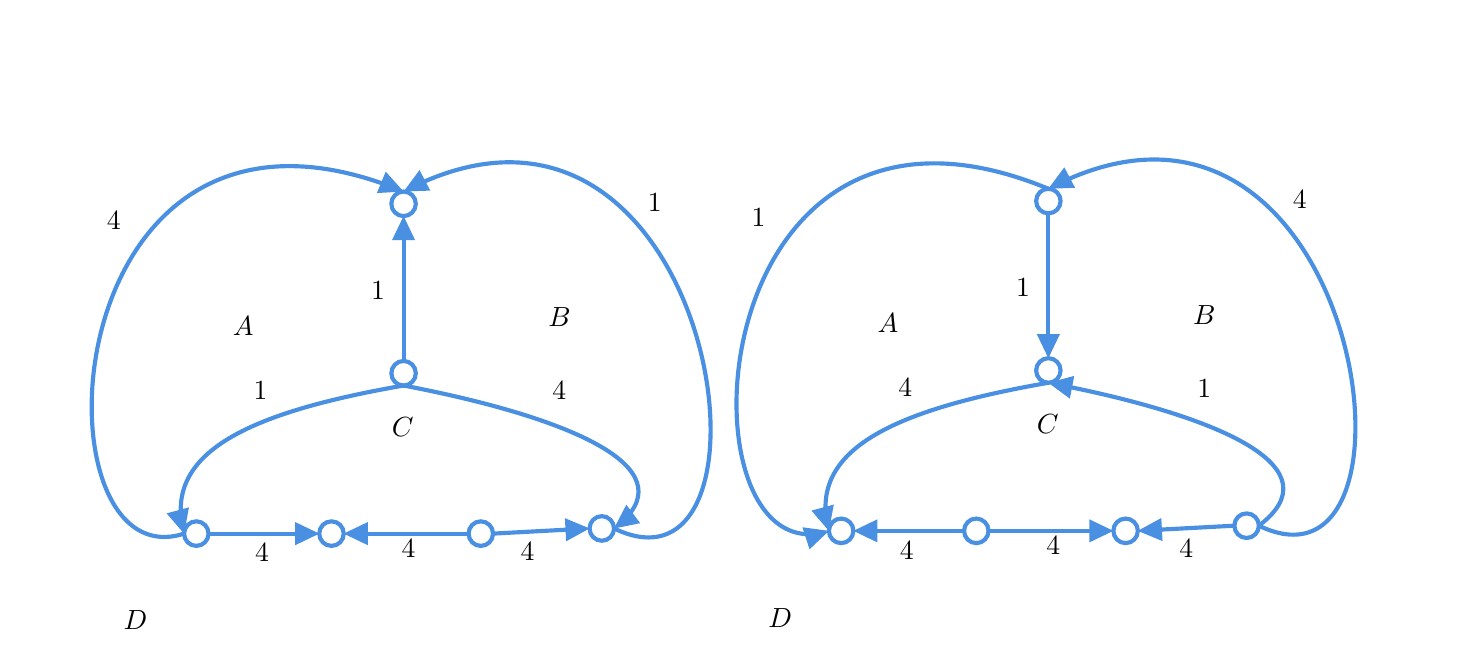
\begin{tikzpicture}[x=0.75pt,y=0.75pt,yscale=-1,xscale=1]
%uncomment if require: \path (0,877); %set diagram left start at 0, and has height of 877

%Shape: Ellipse [id:dp2062482206131232] 
\draw  [color={rgb, 255:red, 74; green, 144; blue, 226 }  ,draw opacity=1 ][line width=1.5]  (181.18,43.69) .. controls (181.18,40.42) and (183.82,37.77) .. (187.08,37.77) .. controls (190.33,37.77) and (192.97,40.42) .. (192.97,43.69) .. controls (192.97,46.95) and (190.33,49.6) .. (187.08,49.6) .. controls (183.82,49.6) and (181.18,46.95) .. (181.18,43.69) -- cycle ;
%Shape: Ellipse [id:dp42181631305663214] 
\draw  [color={rgb, 255:red, 74; green, 144; blue, 226 }  ,draw opacity=1 ][line width=1.5]  (181.18,125.31) .. controls (181.18,122.05) and (183.82,119.39) .. (187.08,119.39) .. controls (190.33,119.39) and (192.97,122.05) .. (192.97,125.31) .. controls (192.97,128.58) and (190.33,131.23) .. (187.08,131.23) .. controls (183.82,131.23) and (181.18,128.58) .. (181.18,125.31) -- cycle ;
%Shape: Ellipse [id:dp1893981875046039] 
\draw  [color={rgb, 255:red, 74; green, 144; blue, 226 }  ,draw opacity=1 ][line width=1.5]  (81.33,202.58) .. controls (81.33,199.31) and (83.97,196.66) .. (87.22,196.66) .. controls (90.48,196.66) and (93.11,199.31) .. (93.11,202.58) .. controls (93.11,205.85) and (90.48,208.5) .. (87.22,208.5) .. controls (83.97,208.5) and (81.33,205.85) .. (81.33,202.58) -- cycle ;
%Shape: Ellipse [id:dp3630097335542829] 
\draw  [color={rgb, 255:red, 74; green, 144; blue, 226 }  ,draw opacity=1 ][line width=1.5]  (276.69,200.09) .. controls (276.69,196.82) and (279.33,194.17) .. (282.59,194.17) .. controls (285.84,194.17) and (288.48,196.82) .. (288.48,200.09) .. controls (288.48,203.36) and (285.84,206.01) .. (282.59,206.01) .. controls (279.33,206.01) and (276.69,203.36) .. (276.69,200.09) -- cycle ;
%Shape: Ellipse [id:dp12213112120599945] 
\draw  [color={rgb, 255:red, 74; green, 144; blue, 226 }  ,draw opacity=1 ][line width=1.5]  (146.45,202.58) .. controls (146.45,199.31) and (149.09,196.66) .. (152.34,196.66) .. controls (155.6,196.66) and (158.24,199.31) .. (158.24,202.58) .. controls (158.24,205.85) and (155.6,208.5) .. (152.34,208.5) .. controls (149.09,208.5) and (146.45,205.85) .. (146.45,202.58) -- cycle ;
%Shape: Ellipse [id:dp14956651149377553] 
\draw  [color={rgb, 255:red, 74; green, 144; blue, 226 }  ,draw opacity=1 ][line width=1.5]  (218.4,202.58) .. controls (218.4,199.31) and (221.03,196.66) .. (224.29,196.66) .. controls (227.54,196.66) and (230.18,199.31) .. (230.18,202.58) .. controls (230.18,205.85) and (227.54,208.5) .. (224.29,208.5) .. controls (221.03,208.5) and (218.4,205.85) .. (218.4,202.58) -- cycle ;
%Curve Lines [id:da46118430818328493] 
\draw [color={rgb, 255:red, 74; green, 144; blue, 226 }  ,draw opacity=1 ][line width=1.5]    (80.43,198.63) .. controls (73.79,162.96) and (112.86,144.16) .. (187.08,131.23) ;
\draw [shift={(81.33,202.58)}, rotate = 254.88] [fill={rgb, 255:red, 74; green, 144; blue, 226 }  ,fill opacity=1 ][line width=0.08]  [draw opacity=0] (11.61,-5.58) -- (0,0) -- (11.61,5.58) -- cycle    ;
%Curve Lines [id:da12684350601217753] 
\draw [color={rgb, 255:red, 74; green, 144; blue, 226 }  ,draw opacity=1 ][line width=1.5]    (292.05,197.16) .. controls (321.77,170.32) and (267.27,146.57) .. (187.08,131.23) ;
\draw [shift={(288.48,200.09)}, rotate = 323] [fill={rgb, 255:red, 74; green, 144; blue, 226 }  ,fill opacity=1 ][line width=0.08]  [draw opacity=0] (11.61,-5.58) -- (0,0) -- (11.61,5.58) -- cycle    ;
%Curve Lines [id:da12533726813089074] 
\draw [color={rgb, 255:red, 74; green, 144; blue, 226 }  ,draw opacity=1 ][line width=1.5]    (288.48,200.09) .. controls (375.8,242.25) and (338.78,-38.85) .. (189.34,36.6) ;
\draw [shift={(187.08,37.77)}, rotate = 332.3] [fill={rgb, 255:red, 74; green, 144; blue, 226 }  ,fill opacity=1 ][line width=0.08]  [draw opacity=0] (11.61,-5.58) -- (0,0) -- (11.61,5.58) -- cycle    ;
%Curve Lines [id:da052098391594170956] 
\draw [color={rgb, 255:red, 74; green, 144; blue, 226 }  ,draw opacity=1 ][line width=1.5]    (81.33,202.58) .. controls (6.97,226.76) and (15.81,-30.37) .. (184.52,36.73) ;
\draw [shift={(187.08,37.77)}, rotate = 202.45] [fill={rgb, 255:red, 74; green, 144; blue, 226 }  ,fill opacity=1 ][line width=0.08]  [draw opacity=0] (11.61,-5.58) -- (0,0) -- (11.61,5.58) -- cycle    ;
%Straight Lines [id:da025851980169662614] 
\draw [color={rgb, 255:red, 74; green, 144; blue, 226 }  ,draw opacity=1 ][line width=1.5]    (93.11,202.58) -- (142.45,202.58) ;
\draw [shift={(146.45,202.58)}, rotate = 180] [fill={rgb, 255:red, 74; green, 144; blue, 226 }  ,fill opacity=1 ][line width=0.08]  [draw opacity=0] (11.61,-5.58) -- (0,0) -- (11.61,5.58) -- cycle    ;
%Straight Lines [id:da7108101232087555] 
\draw [color={rgb, 255:red, 74; green, 144; blue, 226 }  ,draw opacity=1 ][line width=1.5]    (162.24,202.58) -- (218.4,202.58) ;
\draw [shift={(158.24,202.58)}, rotate = 0] [fill={rgb, 255:red, 74; green, 144; blue, 226 }  ,fill opacity=1 ][line width=0.08]  [draw opacity=0] (11.61,-5.58) -- (0,0) -- (11.61,5.58) -- cycle    ;
%Straight Lines [id:da4593573245399082] 
\draw [color={rgb, 255:red, 74; green, 144; blue, 226 }  ,draw opacity=1 ][line width=1.5]    (230.18,202.58) -- (272.7,200.3) ;
\draw [shift={(276.69,200.09)}, rotate = 176.93] [fill={rgb, 255:red, 74; green, 144; blue, 226 }  ,fill opacity=1 ][line width=0.08]  [draw opacity=0] (11.61,-5.58) -- (0,0) -- (11.61,5.58) -- cycle    ;
%Straight Lines [id:da3678344551576813] 
\draw [color={rgb, 255:red, 74; green, 144; blue, 226 }  ,draw opacity=1 ][line width=1.5]    (187.08,119.39) -- (187.08,53.6) ;
\draw [shift={(187.08,49.6)}, rotate = 90] [fill={rgb, 255:red, 74; green, 144; blue, 226 }  ,fill opacity=1 ][line width=0.08]  [draw opacity=0] (11.61,-5.58) -- (0,0) -- (11.61,5.58) -- cycle    ;
%Shape: Ellipse [id:dp5834798930697471] 
\draw  [color={rgb, 255:red, 74; green, 144; blue, 226 }  ,draw opacity=1 ][line width=1.5]  (491.85,42.35) .. controls (491.85,39.08) and (494.49,36.43) .. (497.74,36.43) .. controls (501,36.43) and (503.63,39.08) .. (503.63,42.35) .. controls (503.63,45.62) and (501,48.27) .. (497.74,48.27) .. controls (494.49,48.27) and (491.85,45.62) .. (491.85,42.35) -- cycle ;
%Shape: Ellipse [id:dp9667981945481139] 
\draw  [color={rgb, 255:red, 74; green, 144; blue, 226 }  ,draw opacity=1 ][line width=1.5]  (491.85,123.98) .. controls (491.85,120.71) and (494.49,118.06) .. (497.74,118.06) .. controls (501,118.06) and (503.63,120.71) .. (503.63,123.98) .. controls (503.63,127.25) and (501,129.9) .. (497.74,129.9) .. controls (494.49,129.9) and (491.85,127.25) .. (491.85,123.98) -- cycle ;
%Shape: Ellipse [id:dp09059574964185924] 
\draw  [color={rgb, 255:red, 74; green, 144; blue, 226 }  ,draw opacity=1 ][line width=1.5]  (392,201.25) .. controls (392,197.98) and (394.64,195.33) .. (397.89,195.33) .. controls (401.14,195.33) and (403.78,197.98) .. (403.78,201.25) .. controls (403.78,204.52) and (401.14,207.17) .. (397.89,207.17) .. controls (394.64,207.17) and (392,204.52) .. (392,201.25) -- cycle ;
%Shape: Ellipse [id:dp3605131756242862] 
\draw  [color={rgb, 255:red, 74; green, 144; blue, 226 }  ,draw opacity=1 ][line width=1.5]  (587.36,198.76) .. controls (587.36,195.49) and (590,192.84) .. (593.25,192.84) .. controls (596.51,192.84) and (599.15,195.49) .. (599.15,198.76) .. controls (599.15,202.03) and (596.51,204.68) .. (593.25,204.68) .. controls (590,204.68) and (587.36,202.03) .. (587.36,198.76) -- cycle ;
%Shape: Ellipse [id:dp6418673252768715] 
\draw  [color={rgb, 255:red, 74; green, 144; blue, 226 }  ,draw opacity=1 ][line width=1.5]  (457.12,201.25) .. controls (457.12,197.98) and (459.76,195.33) .. (463.01,195.33) .. controls (466.27,195.33) and (468.9,197.98) .. (468.9,201.25) .. controls (468.9,204.52) and (466.27,207.17) .. (463.01,207.17) .. controls (459.76,207.17) and (457.12,204.52) .. (457.12,201.25) -- cycle ;
%Shape: Ellipse [id:dp39805151621059387] 
\draw  [color={rgb, 255:red, 74; green, 144; blue, 226 }  ,draw opacity=1 ][line width=1.5]  (529.06,201.25) .. controls (529.06,197.98) and (531.7,195.33) .. (534.95,195.33) .. controls (538.21,195.33) and (540.85,197.98) .. (540.85,201.25) .. controls (540.85,204.52) and (538.21,207.17) .. (534.95,207.17) .. controls (531.7,207.17) and (529.06,204.52) .. (529.06,201.25) -- cycle ;
%Curve Lines [id:da1957524342127539] 
\draw [color={rgb, 255:red, 74; green, 144; blue, 226 }  ,draw opacity=1 ][line width=1.5]    (391.09,197.3) .. controls (384.45,161.63) and (423.53,142.83) .. (497.74,129.9) ;
\draw [shift={(392,201.25)}, rotate = 254.88] [fill={rgb, 255:red, 74; green, 144; blue, 226 }  ,fill opacity=1 ][line width=0.08]  [draw opacity=0] (11.61,-5.58) -- (0,0) -- (11.61,5.58) -- cycle    ;
%Curve Lines [id:da3321764957558633] 
\draw [color={rgb, 255:red, 74; green, 144; blue, 226 }  ,draw opacity=1 ][line width=1.5]    (599.15,198.76) .. controls (635.8,171.14) and (582.49,146.54) .. (501.46,130.62) ;
\draw [shift={(497.74,129.9)}, rotate = 10.82] [fill={rgb, 255:red, 74; green, 144; blue, 226 }  ,fill opacity=1 ][line width=0.08]  [draw opacity=0] (11.61,-5.58) -- (0,0) -- (11.61,5.58) -- cycle    ;
%Curve Lines [id:da2799756577005189] 
\draw [color={rgb, 255:red, 74; green, 144; blue, 226 }  ,draw opacity=1 ][line width=1.5]    (599.15,198.76) .. controls (686.47,240.92) and (649.45,-40.18) .. (500,35.27) ;
\draw [shift={(497.74,36.43)}, rotate = 332.3] [fill={rgb, 255:red, 74; green, 144; blue, 226 }  ,fill opacity=1 ][line width=0.08]  [draw opacity=0] (11.61,-5.58) -- (0,0) -- (11.61,5.58) -- cycle    ;
%Curve Lines [id:da9026596524821855] 
\draw [color={rgb, 255:red, 74; green, 144; blue, 226 }  ,draw opacity=1 ][line width=1.5]    (387.62,202.37) .. controls (317.7,215.29) and (329.99,-32.88) .. (497.74,36.43) ;
\draw [shift={(392,201.25)}, rotate = 161.99] [fill={rgb, 255:red, 74; green, 144; blue, 226 }  ,fill opacity=1 ][line width=0.08]  [draw opacity=0] (11.61,-5.58) -- (0,0) -- (11.61,5.58) -- cycle    ;
%Straight Lines [id:da29172929203159703] 
\draw [color={rgb, 255:red, 74; green, 144; blue, 226 }  ,draw opacity=1 ][line width=1.5]    (407.78,201.25) -- (457.12,201.25) ;
\draw [shift={(403.78,201.25)}, rotate = 0] [fill={rgb, 255:red, 74; green, 144; blue, 226 }  ,fill opacity=1 ][line width=0.08]  [draw opacity=0] (11.61,-5.58) -- (0,0) -- (11.61,5.58) -- cycle    ;
%Straight Lines [id:da23336632170754767] 
\draw [color={rgb, 255:red, 74; green, 144; blue, 226 }  ,draw opacity=1 ][line width=1.5]    (468.9,201.25) -- (525.06,201.25) ;
\draw [shift={(529.06,201.25)}, rotate = 180] [fill={rgb, 255:red, 74; green, 144; blue, 226 }  ,fill opacity=1 ][line width=0.08]  [draw opacity=0] (11.61,-5.58) -- (0,0) -- (11.61,5.58) -- cycle    ;
%Straight Lines [id:da7582939485718254] 
\draw [color={rgb, 255:red, 74; green, 144; blue, 226 }  ,draw opacity=1 ][line width=1.5]    (544.84,201.03) -- (587.36,198.76) ;
\draw [shift={(540.85,201.25)}, rotate = 356.93] [fill={rgb, 255:red, 74; green, 144; blue, 226 }  ,fill opacity=1 ][line width=0.08]  [draw opacity=0] (11.61,-5.58) -- (0,0) -- (11.61,5.58) -- cycle    ;
%Straight Lines [id:da2633005133934979] 
\draw [color={rgb, 255:red, 74; green, 144; blue, 226 }  ,draw opacity=1 ][line width=1.5]    (497.74,114.06) -- (497.74,48.27) ;
\draw [shift={(497.74,118.06)}, rotate = 270] [fill={rgb, 255:red, 74; green, 144; blue, 226 }  ,fill opacity=1 ][line width=0.08]  [draw opacity=0] (11.61,-5.58) -- (0,0) -- (11.61,5.58) -- cycle    ;

% Text Node
\draw (103.33,96.4) node [anchor=north west][inner sep=0.75pt]    {$A$};
% Text Node
\draw (255.33,92.4) node [anchor=north west][inner sep=0.75pt]    {$B$};
% Text Node
\draw (180,145.07) node [anchor=north west][inner sep=0.75pt]    {$C$};
% Text Node
\draw (50.67,238.4) node [anchor=north west][inner sep=0.75pt]    {$D$};
% Text Node
\draw (303.33,37.4) node [anchor=north west][inner sep=0.75pt]    {$1$};
% Text Node
\draw (113.33,127.73) node [anchor=north west][inner sep=0.75pt]    {$1$};
% Text Node
\draw (257.33,128.07) node [anchor=north west][inner sep=0.75pt]    {$4$};
% Text Node
\draw (42.67,46.07) node [anchor=north west][inner sep=0.75pt]    {$4$};
% Text Node
\draw (114,206.07) node [anchor=north west][inner sep=0.75pt]    {$4$};
% Text Node
\draw (184.67,204.07) node [anchor=north west][inner sep=0.75pt]    {$4$};
% Text Node
\draw (242,205.4) node [anchor=north west][inner sep=0.75pt]    {$4$};
% Text Node
\draw (170,79.73) node [anchor=north west][inner sep=0.75pt]    {$1$};
% Text Node
\draw (414,95.07) node [anchor=north west][inner sep=0.75pt]    {$A$};
% Text Node
\draw (566,91.07) node [anchor=north west][inner sep=0.75pt]    {$B$};
% Text Node
\draw (490.67,143.73) node [anchor=north west][inner sep=0.75pt]    {$C$};
% Text Node
\draw (361.33,237.07) node [anchor=north west][inner sep=0.75pt]    {$D$};
% Text Node
\draw (614,36.07) node [anchor=north west][inner sep=0.75pt]    {$4$};
% Text Node
\draw (424,126.4) node [anchor=north west][inner sep=0.75pt]    {$4$};
% Text Node
\draw (568,126.73) node [anchor=north west][inner sep=0.75pt]    {$1$};
% Text Node
\draw (353.33,44.73) node [anchor=north west][inner sep=0.75pt]    {$1$};
% Text Node
\draw (424.67,204.73) node [anchor=north west][inner sep=0.75pt]    {$4$};
% Text Node
\draw (495.33,202.73) node [anchor=north west][inner sep=0.75pt]    {$4$};
% Text Node
\draw (559.33,204.07) node [anchor=north west][inner sep=0.75pt]    {$4$};
% Text Node
\draw (480.67,78.4) node [anchor=north west][inner sep=0.75pt]    {$1$};


\end{tikzpicture}
        \caption{Descompocision reduciendo las caras de dos aristas}
    \end{figure}
    
\end{eg}
Observe que particularmente este proceso es primero bastante mas fácil de realizar de lo que en un principio se podría pensar, pero ademas de esto, nos da una descompocision relativamente sencilla que nos permite visualizar la tres variedad, y no solo eso, nos da indicios de un análogo de la descomposición de dos variedades por medio de triangulaciones. Un comentario extra es que esta construcción también funciona en nudos y enlaces alternantes salvo que hay que hacer simplificaciones similares a la reducción de caras donde solo hay dos lados.